%============================ MAIN DOCUMENT ================================
% define document class
\PassOptionsToPackage{table}{xcolor}
\documentclass[
  a4paper,
  BCOR=15mm,            % Binding correction
  twoside,
% openright,
%  headings=openright,
  bibliography=totoc,   % If enabled add bibliography to TOC
  listof=totoc,         % If enabled add lists to TOC
  monolingual,
% bilingual,
  invert-title,
]{bfhthesis}

\usepackage[
top=25mm,
bottom=25mm,
footskip=10mm % Abstand des Fußzeilentextes vom Haupttext
]{geometry}


\LoadBFHModule{listings,terminal,boxes}
%---------------------------------------------------------------------------
% Documents paths
%---------------------------------------------------------------------------
\makeatletter
\def\input@path{{content/}}
%or: \def\input@path{{/path/to/folder/}{/path/to/other/folder/}}
\makeatother
%-----------------  Base packages     --------------------------------------
% Include Packages
\usepackage[french,ngerman,main=ngerman]{babel}  % https://www.namsu.de/Extra/pakete/Babel.html
%% To disable the french list setting you can add -- see https://gitlab.ti.bfh.ch/bfh-latex/bfh-ci/-/issues/166
%\frenchsetup{StandardLists=true}

\usepackage{amsmath}          % various features to facilitate writing math formulas
\usepackage{amsthm}           % enhanced version of latex's newtheorem
\usepackage{amsfonts}         % set of miscellaneous TeX fonts that augment the standard CM
\usepackage{amssymb}          % mathematical special characters

\usepackage{siunitx}

\usepackage{graphicx}         % integration of images
\usepackage{float}            % floating objects

\usepackage{caption}          % for captions of figures and tables
\usepackage{subcaption}       % for subcaptions in subfigures
\usepackage{cite}             % use bibtex
\usepackage{lipsum, wrapfig}

\usepackage{exscale}          % mathematical size corresponds to textsize
\usepackage{multirow}         % multirow emables combining rows in tables
\usepackage{multicol}
\usepackage{makecell}

\usepackage{longtable}

\usepackage{parskip}

\usepackage{tabularx}
\usepackage{graphicx}
\usepackage{float}
\usepackage[flushleft]{threeparttable}

%---------------------------------------------------------------------------
% Graphics paths
%---------------------------------------------------------------------------
\graphicspath{{pictures/}{figures/}}
%---------------------------------------------------------------------------
% Blind text -> for dummy text
%---------------------------------------------------------------------------
\usepackage{blindtext}    
\usepackage{letltxmacro}   
\LetLtxMacro{\blindtextblindtext}{\blindtext}

\RenewDocumentCommand{\blindtext}{O{\value{blindtext}}}{
	\begingroup\color{BFH-Gray}\blindtextblindtext[#1]\endgroup
}
%---------------------------------------------------------------------------
% Glossary Package
%---------------------------------------------------------------------------
% the glossaries package uses makeindex
% if you use TeXnicCenter do the following steps:
%  - Goto "Ausgabeprofile definieren" (ctrl + F7)
%  - Select the profile "LaTeX => PDF"
%  - Add in register "Nachbearbeitung" a new "Postprozessoren" point named Glossar
%  - Select makeindex.exe in the field "Anwendung" ( ..\MiKTeX x.x\miktex\bin\makeindex.exe )
%  - Add this [ -s "%tm.ist" -t "%tmx.glg" -o "%tm.gls" "%tm.glo" ] in the field "Argumente"
%
% for futher informations go to http://ewus.de/tipp-1029.html
%---------------------------------------------------------------------------
\usepackage[nonumberlist]{glossaries-extra}
\makeglossaries
\newglossaryentry{BibTeX}{
  name={BibTeX},
  description={Program for the creation of bibliographical references and directories in \TeX or \LaTeX\, documents},
  plural=BibTeXs
}

\newglossaryentry{zynq}{
  name=Zynq,
  description={\textbf{Zynq} Xilinx' AP SoC. The characteristic feature of Zynq is that it combines a dual-core ARM Cortex-A9 processor with traditional Series-7 FPGA logic fabric},
  plural=Zynqs
}


\newglossaryentry{soc}{
  name=SoC,
  description={\textbf{System-on-Chip (SoC)} A single chip that holds all of the necessary hardware and electronic circuitry for a complete system. SoC includes on-chip memory (RAM and ROM), the microprocessor, peripheral interfaces, I/O logic control, data converters, and other components that comprise a complete computer system},
  plural=SoCs
}

\newglossaryentry{apsoc}{
  name=AP SoC,
  description={\textbf{All Programmable System-on-Chip (AP SoC)} was introduced by Xilinx. It represents a IC which comprise a hard-core processor core surrounded by an FPGA fabric. This type of ICs are highly configurable and provide algorithm partitioning capabilities. This provides high benefit for highly scale-able applications as well as fast time-to-market},
  plural=AP SoCs
}

\newglossaryentry{zbook}{
  name=Zynq Book,
  description={\textbf{Zynq Book} A book that summarizes all the important aspects when working with Zynq and provides a strong and easy understandable introduction to the topic. The book has been written by a team of University of Strathclyde Glasgow in cooperation with Xilinx},
  plural=Zynq Books
}

\newglossaryentry{zboard}{
  name=ZedBoard,
  description={\textbf{ZedBoard} A low cost development board featuring a Zynq-700 0 SoC, and a number of peripherals},
  plural=ZedBoards
}


\newglossaryentry{asic}{
  name=ASIC,
  description={\textbf{Application-Specific Integrated Circuit (ASIC)} An integrated circuit which is designed for a specific use, rather than general-purpose use},
  plural=ASICs
}

\newglossaryentry{rtos}{
  name=RTOS,
  description={\textbf{Real-Time Operating System (RTOS)} A category of operating systems defined by their ability to respond quickly and predictably for a given task},
  plural=RTOSs
}

\newglossaryentry{arm}{
  name=ARM,
  description={\textbf{ARM} A family of processor architectures. The hard processor type which forms the basis of the Zynq processing system is an ARM Cortex-A9 version. The term ‘ARM’ may also be used to refer to the developer of the processor, i.e. a company of the same name}
}

%---------------------------------------------------------------------------
% Makeindex Package
%---------------------------------------------------------------------------
\usepackage{makeidx}
\makeindex
%\usepackage{imakeidx}          % To produce index
%\makeindex[columns=2,intoc]    % Index-Initialisation
%\makeindex[columns=3,columnseprule,columnsep,intoc]
%---------------------------------------------------------------------------
% Hyperref Package (Create links in a pdf)
%---------------------------------------------------------------------------
\usepackage[
	,bookmarks
	,plainpages=false
	,pdfpagelabels
    ,pdfusetitle
	,backref = {false}          % No index backreference
	,colorlinks = {true}        % Color links in a PDF
	,hypertexnames = {true}     % no failures "same page(i)"
	,bookmarksopen = {true}     % opens the bar on the left side
	,bookmarksopenlevel = {0}   % depth of opened bookmarks
	,linkcolor=.
	,filecolor=.
	,urlcolor=.
	,citecolor=.
]{hyperref}
%---------------------------------------------------------------------------

%% %% Customize Footer and Headers in Document
%% \KOMAoptions{headsepline,plainheadsepline,footsepline,plainfootsepline}%
%% \setkomafont{headsepline}{\color{BFH-DarkBlue}}% BFH-DarkBlue required bfhcolors
%% \setkomafont{footsepline}{\color{BFH-DarkBlue}}%
%% \lehead*{lehead} % the * character does replace the header on the first chapter page as well
%% \cehead*{cehead}
%% \rehead*{rehead}
%% \lohead*{lohead}
%% \cohead*{cohead}
%% \rohead*{rohead}

%% \lefoot*{lefoot}
%% \cefoot*{cefoot}
%% \refoot*{refoot}
%% \lofoot*{lofoot}
%% \cofoot*{cofoot}
%% \rofoot*{rofoot}
%---------------------------------------------------------------------------
\begin{document}

%% Snippet do redefine German babel translations -- see FAQ latex.ti.bfh.ch for further information or
%% the package documentation https://www.ctan.org/pkg/translations
%% \redefinetranslation{German}{Advisor}{Dozentin}
%% \redefinetranslation{German}{advisor}{Dozentin} %  just for consistency
%% \redefinetranslation{German}{Author}{Autorin}
%% \redefinetranslation{German}{author}{Autorin} %  just for consistency
%% \redefinetranslation{German}{Co-advisor}{Mitbetreuerin}
%% \redefinetranslation{German}{co-advisor}{Mitbetreuerin} %  just for consistency
%% \redefinetranslation{German}{Expert}{Expertin}
%% \redefinetranslation{German}{expert}{Expertin} %  just for consistency
%% \redefinetranslation{German}{Project partner}{Projektpartnerin}
%% \redefinetranslation{German}{project partner}{Projektpartnerin} %  just for consistency

%------------ START FRONT PART ------------
\frontmatter

\title{MSE-Master-Thesis}
\subtitle{Skillbasierter Robotereinsatz für Industrieaufgaben}
\author{Spatz Yannick}
\institution{Bern University of Applied Sciences}
\department{Technik und Informatik}
\institute{Automation und Mechatronik}
\version{1.0}
\titlegraphic*{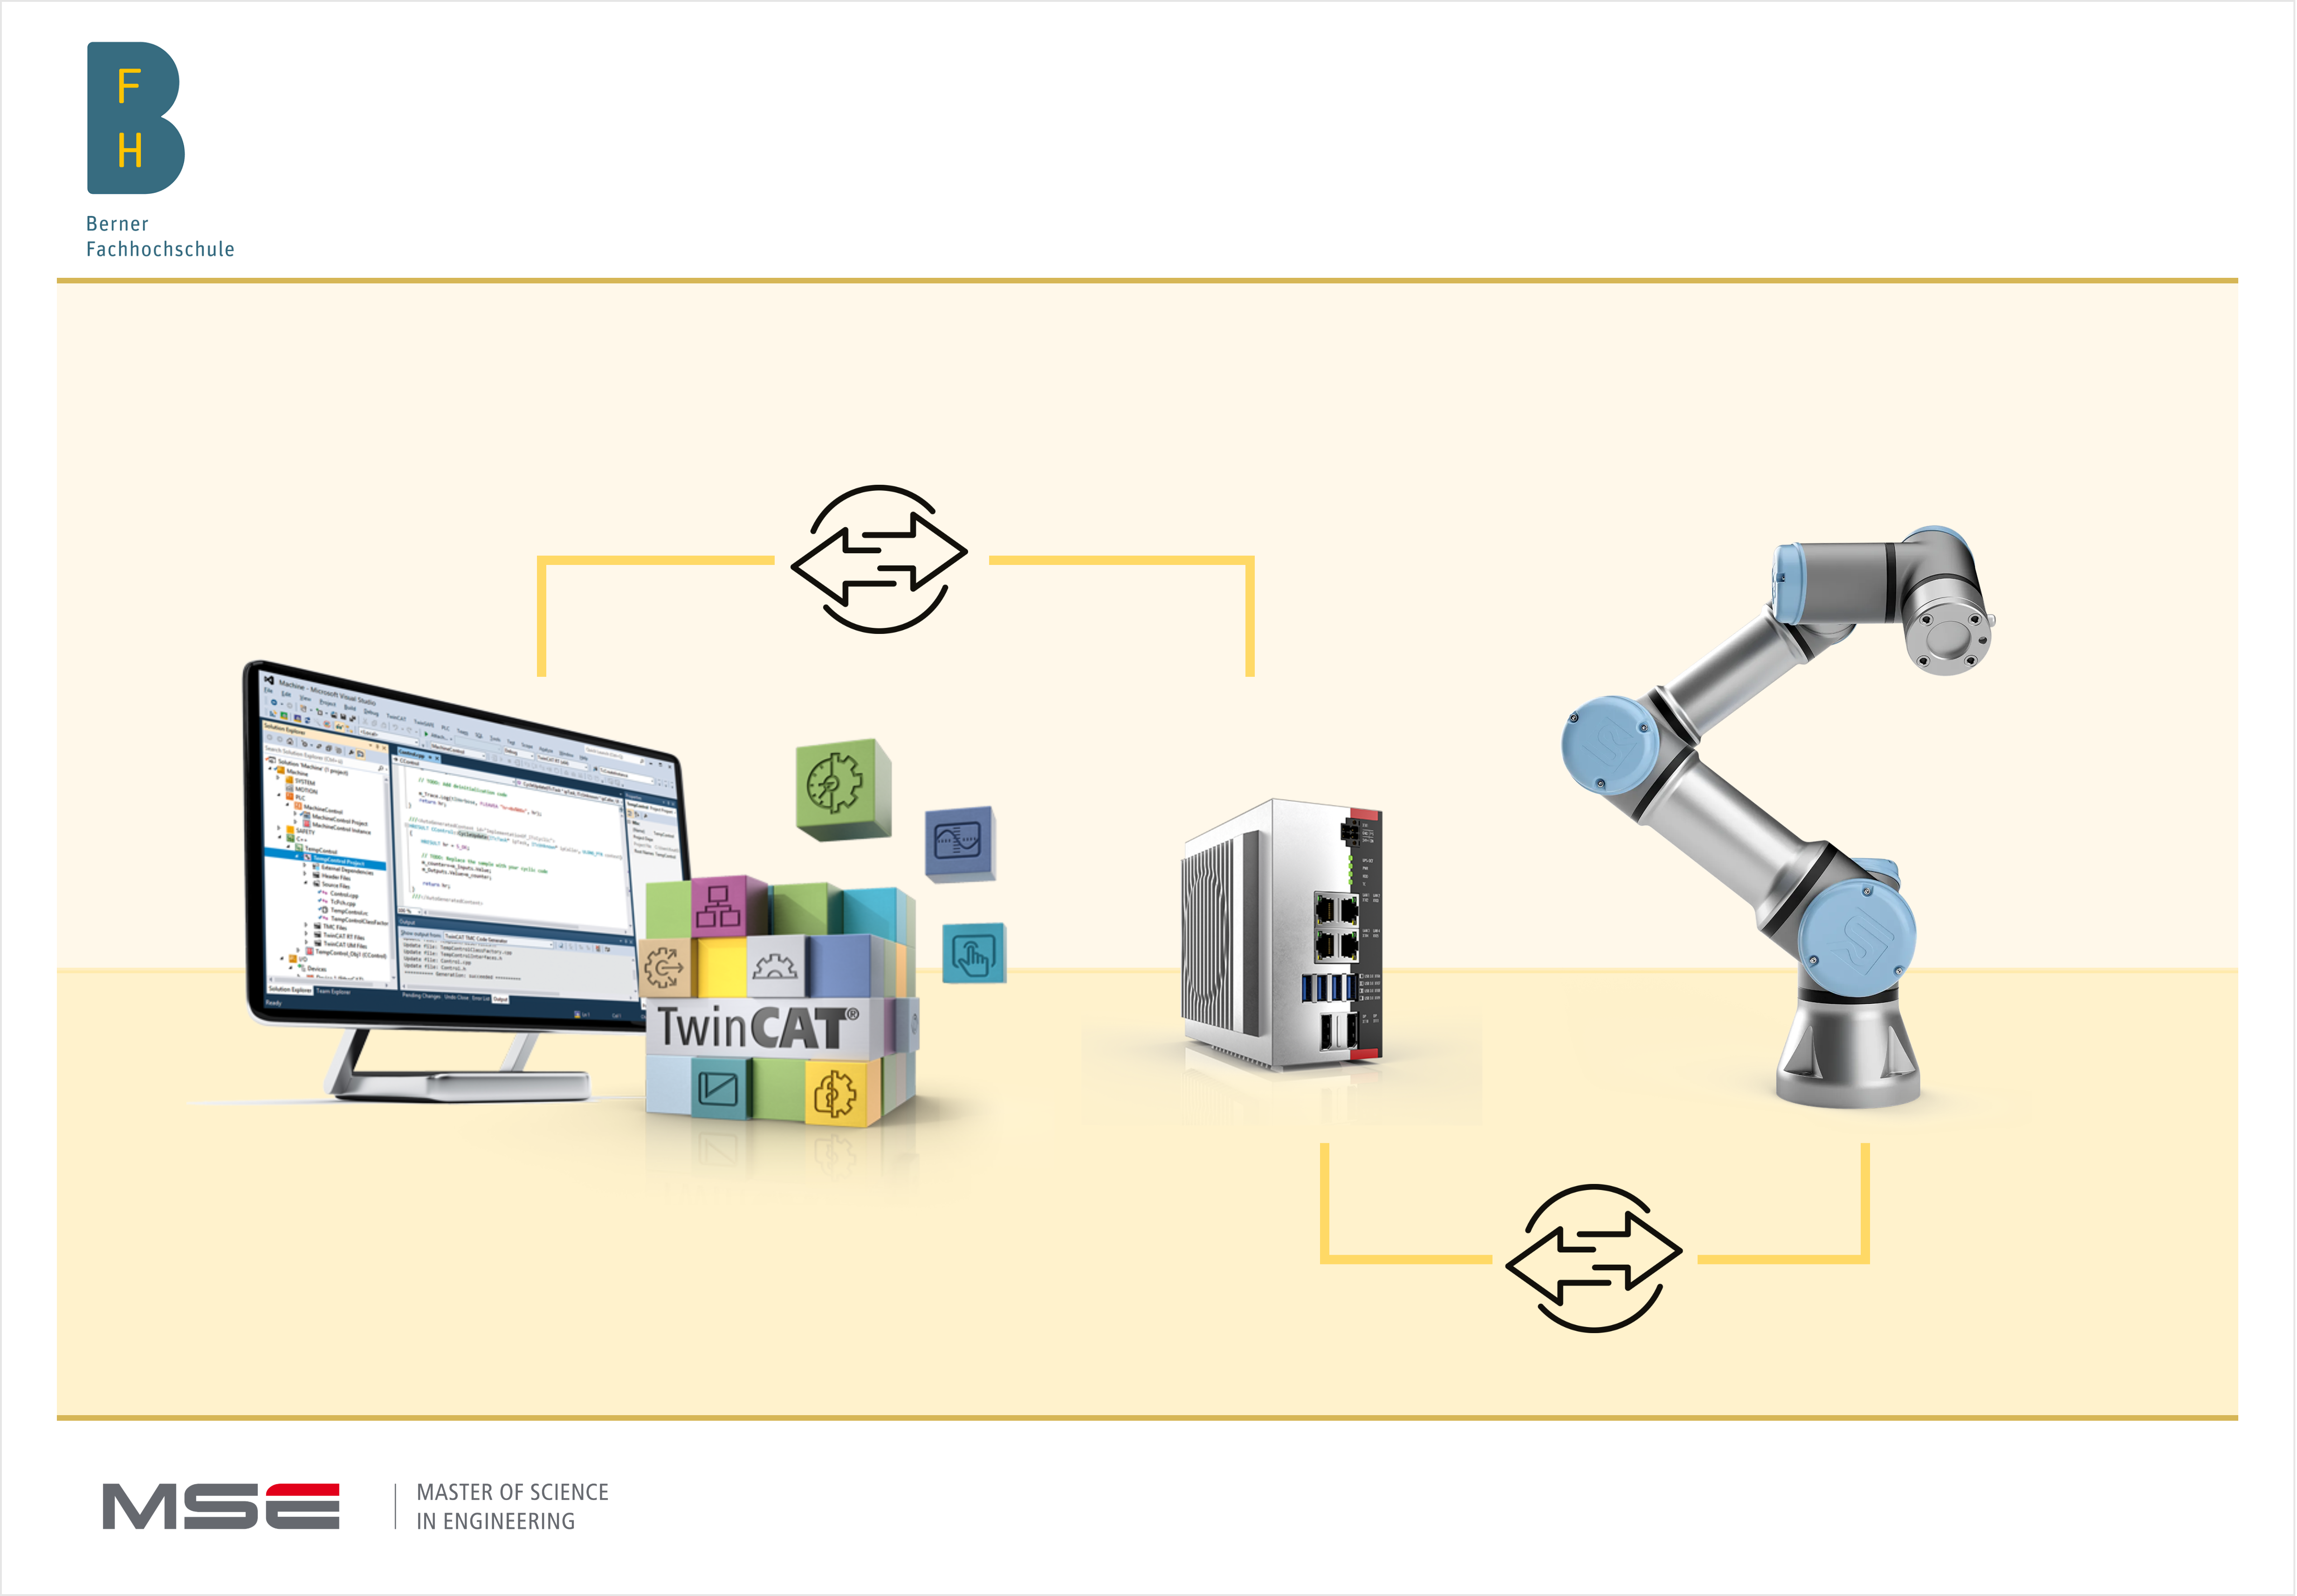
\includegraphics{Titelbild}}
\advisor{Prof. Borer Melchior}
\expert{Stucki Simon}
\degreeprogram{Master of Science in Engineering}
\setupSignature{
	Yannick Spatz={
\includegraphics[width=.7\linewidth]{Unterschrift}}
}


%----------------  BFH tile page   -----------------------------------------
\maketitle
%------------ ABSTRACT        ----------------
\addchap{Abstract}
One-paragraph summary of the entire study – typically no more than 250 words in length (and in many cases it is well shorter than that), the Abstract provides an overview of the study.


%------------ TABLEOFCONTENTS ----------------
\tableofcontents

%------------ START MAIN PART ------------
\mainmatter

\chapter{Rahmen der Arbeit} \label{Rahmen der Arbeit}
\section{Einleitung in die Thesis} \label{Einleitung in die Thesis}

Das Institut für Intelligente Industrielle Systeme (I3S) befasste sich im Rahmen von Forschungsprojekten bereits mit der Thematik von skill-basierten Softwareansätzen. ROS war dabei ein zentrales Element der Entwicklung. Jedoch gab es weiterhin viele offene Fragen in Bezug auf den Einsatz von Skills. 
\\
Die Thesis wird mit der Idee initialisiert, neue Ansätze und Herangehensweisen zu finden und zu erarbeiten. Der Fokus liegt auf einer industrienahen Umsetzung und den Einsatz einer SPS. Bereits gewonnene Erfahrungen aus Projekten im Bereich der Verfahrenstechnik sollen in die Entwicklung neuer Ansätze einfliessen. Dabei wird die Frage erarbeitet, welche Parallelen es zur Verführungstechnik gibt und wie diese für Skill-Anwendungen übernommen werden könnten. 
 
\vspace{2mm} 
Die Thesis setzt sich mit grundlegenden Fragen auseinander, wie:
\begin{itemize}
	\item Was ist ein Skill und für welche Aufgaben eignet sich der Einsatz dieser.
	\item Wie kann ein Skill definiert werden.
	\item In welche Software-Struktur muss ein Skill eingebettet werden. 
	\item Welche Möglichkeiten und Grenzen hat der Einsatz von Skills.
\end{itemize}
\vspace{3mm} 

Das allgemeine Vorgehen innerhalb des Projektes folgt dabei den klassischen Entwicklungs-Phasen (Analyse / Konzipieren / Ausarbeitung / Auswertung). Zu Beginn wird eine ausführliche Analyse der Thematik, durchgeführt um alle themenrelevanten Fragen zu beantworten. Anhand dieser Analyse werden die diversen Arbeitspakete des Projektes definiert, welche jeweils mit einer Konzept- und Ausarbeitungsphase umgesetzt werden. Die Dokumentation dieser Thesis konzentriert sich darauf, den Entwicklungsprozess sowie die zugrunde liegenden Überlegungen detailliert darzustellen. Der Fokus liegt dabei auf der Beschreibung der methodischen Herangehensweise und der Schritte, die zur Erarbeitung der finalen Lösung geführt haben. Ziel ist es, transparent nachzuvollziehen, wie die Lösung entwickelt wurde und welche Entscheidungen den Prozess geprägt haben.
\\
\\
Mit dem Start des Semesters am 16.09.2024 wurde auch mit der Arbeit an dieser Thesis begonnen. Die Thesis umfasst dabei ca. 900 Arbeitsstunden.  Das Projekt wird von Prof. Melchior Borer betreut und in enger Zusammenarbeit mit dem I3S umgesetzt. Dabei wird ein stetiger Austausch mit Prof. Dr. Norman Urs Baier, dem Leiter des Instituts für Intelligente Industrielle Systeme, angestrebt.  
	
\newpage
\section{Auftragsinterpretation} \label{Auftragsinterpretation}

	\textbf{Problembeschreibung:} \vspace{2mm} 
	\\
	Roboter finden in der Industrie eine immer breiter werdende Anwendung und sind aus vielen Prozessen
	nicht mehr wegzudenken. Ein grosser Beschaffungs- und Inbetriebnahmeaufwand machen es jedoch
	für viele Unternehmen schwierig, einen Roboter in ihre Prozesse zu integrieren. Dadurch werden
	zeitintensive und monotone Arbeiten oftmals noch manuell von Mitarbeitern durchgeführt. Eine grosse
	Hürde des Robotersystems ist der konventionelle Robotersoftwareansatz, welcher ein Grundverständnis
	für die Programmierung des Roboters voraussetzt. Für Veränderungen im Prozessablauf wird dadurch
	zwingend ein Programmierer benötigt.
	\vspace{3mm}
	
	\textbf{Beschreibung des Auftrages:} \vspace{2mm} 
	\\
	Die Thesis beschäftigt sich mit der Frage, wie ein Roboter einfacher und standardisiert programmiert
	werden kann. Hierfür wird der Ansatz einer Rezeptursteuerung (bekannt aus Pharmaprozessen)
	analysiert. Dabei wird untersucht, ob ein solcher Ansatz für Roboteranwendungen geeignet ist und wie
	dieser eingesetzt werden kann. Ein zentrales Element ist dabei der skill-basierte Aufbau eines
	Roboterprogramms.
	\\
	\linebreak
	Die konkreten Ziele dieser Thesis sind wie folgt definiert:
	\begin{itemize}
		\item Analyse des Ansatzes einer Rezeptursteuerung für Roboteranwendungen.
		\item Analyse und Definierung von geeigneten Skills.
		\item Softwaremässige Umsetzung des skill-basierten Ansatzes.
		\item Reaktion der Software auf Fehler des Roboters während der Prozessdurchführung.
	\end{itemize}
	\addvspace{5mm}
	
	\textbf{Auftragskontext:} \vspace{2mm} 
	\\
	Die Thesis findet als BFH-internes Projekt statt, welches aus dem Forschungsprojekt «ACROBA»
	entstanden ist. Das Ziel des ACROBA-Forschungsprojektes ist die Entwicklung und Demonstration neuartiger
	Konzepte für Roboterplattformen bezüglich agiler Fertigung.
	\vspace{3mm}
	
	\textbf{Abgrenzungen:} \vspace{2mm} 
	\\
	Die Thesis beschäftigt sich nicht mit der Umsetzung einer konkreten industriellen Anwendung. Es ist
	jedoch möglich, dass Erkenntnisse aus dieser Thesis für zukünftige Automatisierungsprojekte
	verwendet werden können.
	\vspace{3mm}
	
	\textbf{Projektorganisation:} \vspace{0mm} 
	
	\begin{table}[ht]
		\centering
		\colorlet{BFH-table}{BFH-MediumBlue!10}
		\colorlet{BFH-tablehead}{BFH-MediumBlue!50}
		\begin{bfhTabular}{llll}
			Rolle		& 	Wer							&	Status				&	Kontakt		\\\hline
			
			Advisor		 & Prof. Borer Melchior			& Dozent BFH 			& 	\href{mailto:melchior.borer@bfh.ch}{melchior.borer@bfh.ch}  	\\\hline
			Experte		 & Stucki Simon					& Externer Experte		&	/		\\\hline
			Student		 & Yannick Spatz 				& Master-Student		&	\href{mailto:yannick.spatz@bfh.ch}{yannick.spatz@bfh.ch}	\\\hline
			
		\end{bfhTabular}
		
		\captionsetup{justification=centering}
		\caption{Projektorganisation}
		\label{Projektorganisation}
	\end{table}
	

\section{Zeitplan der Thesis} \label{Zeitplan der Thesis}

	Der erstellte Zeitplan dient als erste grobe Orientierung und stellt eine vorläufige Einschätzung des Projektverlaufs dar. Da der genaue Umfang der Aufgabenstellung für diese Thesis nur schwer im Voraus vollständig abzuschätzen ist, kann der Projektrahmen entsprechend variieren. Insbesondere die Entwicklung der Software ist ein dynamischer und iterativer Prozess.
	\\
	Daher ist der Zeitplan als flexibles Arbeitstool zu verstehen, das zwar eine klare zeitliche Struktur vorgibt, sich jedoch im Laufe des Projekts an veränderte Anforderungen und Erkenntnisse anpassen kann. Er soll einerseits helfen, die einzelnen Meilensteine im Blick zu behalten und andererseits als Leitfaden dienen, um trotz aufkommender Änderungen einen festen Rahmen für den Projektfortschritt zu gewährleisten. Die kontinuierliche Überprüfung und gegebenenfalls Anpassung des Zeitplans ist ein integraler Bestandteil dieses Prozesses, um sicherzustellen, dass das Projekt im vorgesehenen zeitlichen Rahmen bleibt. 

	\begin{figure}[h!]
		\centering
		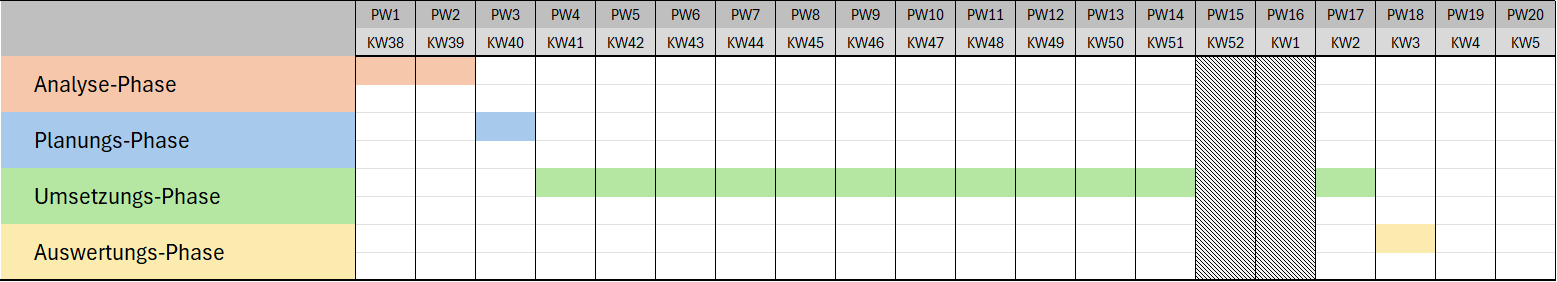
\includegraphics[width=1\textwidth]{01_Rahmen_der_Arbeit/Terminplanung_V2}
		\caption{Grobzeitplan der Thesis}
		\label{fig:Grobzeitplan}
	\end{figure}
	
	\begin{bfhNoteBox}
		Eine detaillierte Version des endgültigen Zeitplans wird im Anhang aufgeführt.
	\end{bfhNoteBox} 

		

\chapter{Einarbeitung in Thematik} \label{Einarbeitung in Thematik}
\section{Vorwissen aus Vorprojekt} \label{Vorwissen aus Vorprojekt}
	Im Rahmen des Master-Projekt 2 wurde eine chemische Reaktoranlage auf Basis von TwinCat automatisiert. Innerhalb des Projekts wurden verschiedene Themen analysiert und erarbeitet, die für diese Thesis von Relevanz sein können.
	\vspace{3mm}
	
	\textbf{Umsetzung einer Rezeptursteuerung:} \vspace{2mm} 
	\\
	Die Anlage wird mit einer Rezeptursteuerung betrieben. Während dem Projekt konnte viel Wissen über die Strukturierung von TwinCAT-Programmen für eine Rezeptursteuerung gesammelt werden. Die korrekte Strukturierung ermöglichst es, anlagenunspezifische Abläufe zu definieren, welche flexibel mit Prozessparametern betrieben werden können. 
	\vspace{3mm}
	
	\textbf{Objektorientierte Struktur:} \vspace{2mm} 
	\\
	Das objektorientierte Programmieren kann ich vielen Programmiersprachen angewendet werden. Es bildet ein essentieller Aspekt einer Rezeptursteuerung und der benötigten Struktur.
	\vspace{3mm}
	
	\textbf{Kommunikation via OPC UA:} \vspace{2mm} 
	\\
	Der Betrieb der Anlage basiert auf der Kommunikation zwischen zwei Ebenen. Die Gesamtsystemebene (Supervisory-Level) definiert über ein Rezept die Prozessparameter. Diese werden via eine OPC-UA-Kommunikationsschnittstelle an die Reaktoreinheitsebene (Control-Level) übergeben, welche die entsprechenden Abläufe startet und schlussendlich mit den Sensoren und Aktoren (Field-Level) interagiert. 
	\vspace{3mm}
	
	Eine ausführlichere Beschreibung der verschiedenen Themen findet sich in der Dokumentation des Master-Projekt 2 (Automatisierung: Chemische Reaktoranlage). Die grundlegende Theorie zu den einzelnen Themen wird in der nachfolgenden Dokumentation  nicht behandelt.
	
\section{Annahmen} \label{Annahmen}
	Obwohl die Thesis keine konkrete praktische Anwendung zum Ziel hat, soll der Auftrag industrienahe umgesetzt werden. Die gewonnenen Erkenntnisse sollen potenziell für zukünftige industrielle Projekte nutzbar sein. Dafür werden verschiedenen Annahmen für die Erarbeitung der Thesis gemacht. 
	\\
	Als Programmierumgebung wird TwinCAT von Beckhoff verwendet, da mit früheren Projekte umfassende Kenntnisse und Erfahrungen mit TwinCAT gesammelt wurden. Das Master-Projekt 2 befasst sich mit der Rezeptursteuerung einer Reaktoranlage, und die dort gewonnenen Erkenntnisse könnten einen erheblichen Mehrwert für die Bearbeitung dieser Thesis bieten. Dank der zahlreichen Zusatzpakete von Beckhoff können viele Funktionalitäten in einer einzigen Software kombiniert werden, wodurch der Einsatz mehrerer verschiedener Software-Tools entfällt.
	\\ 
	Die definierten Annahmen sollen den Rahmen der Thesis klar abstecken, um sicherzustellen, dass innerhalb der zur Verfügung stehenden Zeit ein verwertbares Ergebnis erzielt wird. Trotz dieser Fokussierung wird darauf geachtet, dass die erarbeiteten Strukturen und gewonnenen Erkenntnisse auch auf andere Systeme, abseits von Beckhoff, übertragbar sind. So bleibt die Arbeit nicht nur auf ein spezifisches System beschränkt, sondern bietet Potenzial für eine breitere Anwendung in verschiedenen industriellen Umgebungen.
	

\section{Situationsanalyse} \label{Situationsanalyse}

	\subsection{Fragen bezüglich Referenzprojekt} \label{Fragen bezüglich Referenzprojekt}
	
	\textbf{Frage 1.1:} Was ist ein chargenorientierter Ansatz nach ANSI/ISA-88 \vspace{2mm} 
	\\
		Der internationale Standard ANSI/ISA-88 beschreibt Methoden und Strukturen zur Entwerfung von Chargensteuerungen in der Pharma- und Chemieindustrie. Eine Charge ist in diesem Kontext eine definierte Produktionsmenge, welche innerhalb eines Produktionsablaufes prozessiert wird.  Das Rezept beschreibt dabei den Herstellungsweg einer Charge und definiert die notwendigen Prozessinformationen. 
		
		\begin{figure}[h!]
			\centering
			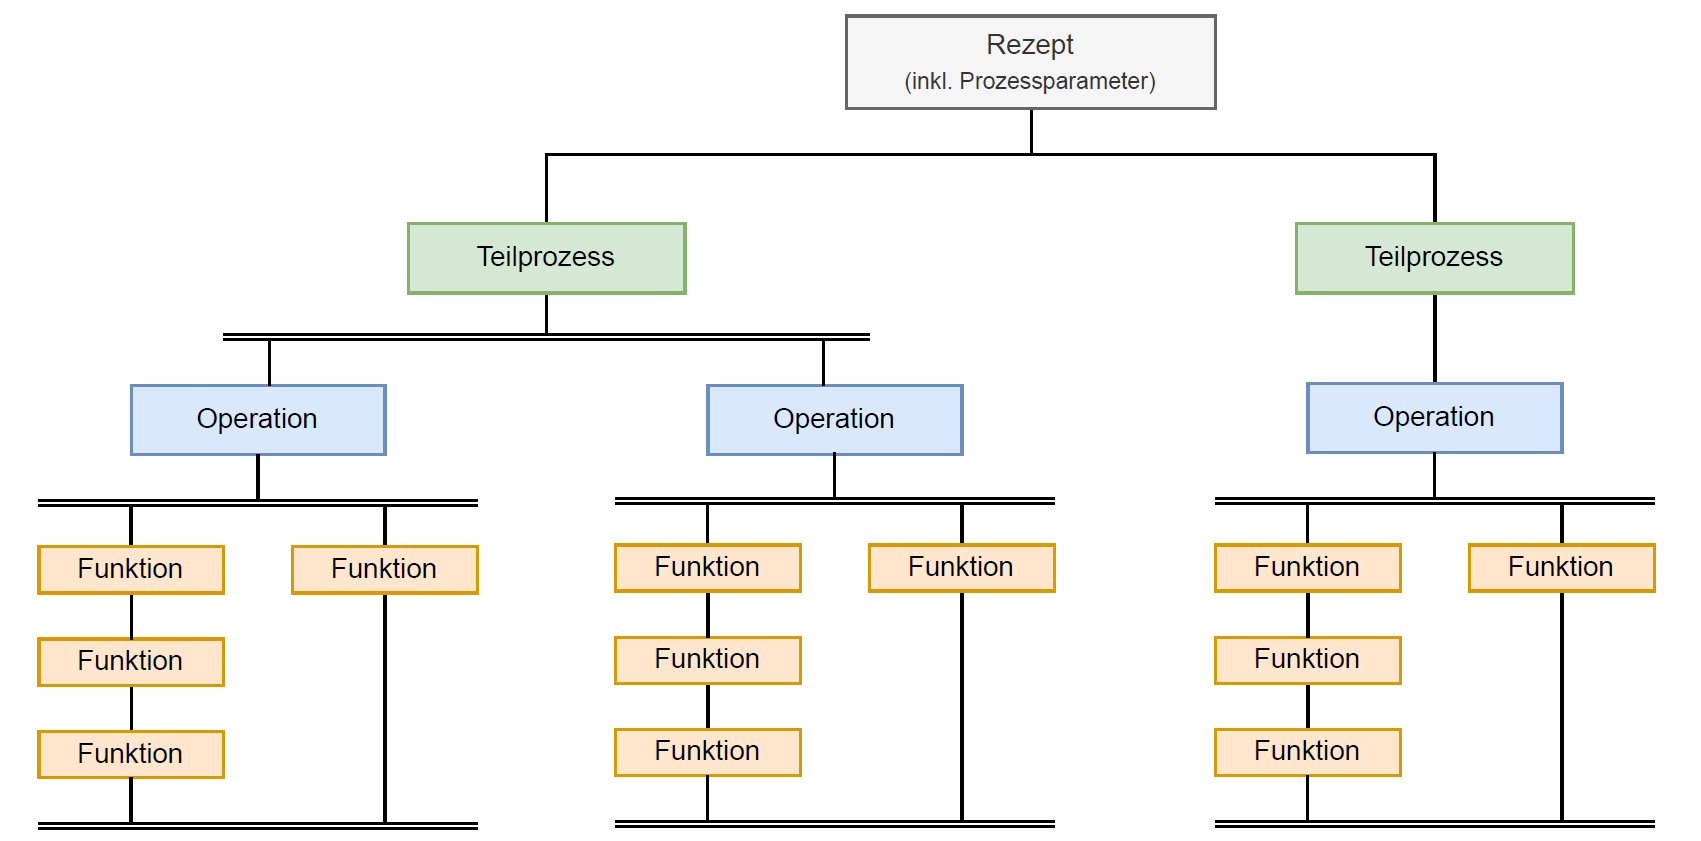
\includegraphics[width=0.8\textwidth]{02_Einfuehrung_in_Thematik/ISA88Struktur}
			\captionsetup{justification=centering}
			\caption{Prozessstruktur von ISA-88}
			\label{fig:Prozessstruktur_ISA88}
		\end{figure}
		
		Das Rezept besteht aus unterschiedlichen Teilprozessen, welche aus Operationen zusammengesetzt sind (\ref{fig:Prozessstruktur_ISA88}). Auf der untersten Stufen befinden sich die Funktionen. Diese stellen die Grundfunktionalitäten der Anlagenkomponenten dar, z.B. das Öffnen und Schliessen eines Ventiles. Alle Prozesse können seriell oder parallel durchgeführt werden. Durch diese Struktur wird der Prozess nicht mit einem fest definierten Ablauf gesteuert, sondern durch die im Rezept definierten Schritte und Parameter. Dies ermöglicht ein flexibles Einsetzen der Anlage und deren Ressourcen. Sofern es die Infrastruktur der Anlage zulässt, kann jedes Rezept gefahren werden. Dies reduziert Stillstandszeiten der Anlage und macht diese effizienter. Dieses Prinzip kann so erweitert werden, dass das System auch selbständig die Anlagenelemente definiert, welche für das Prozessieren der Charge verwendet werden. Hierbei spricht man dann von einer Rezeptur und nicht mehr von einem Rezept. Besteht das System zum Beispiel aus mehreren chemischen Reaktoren, entscheidet die Rezeptur selbständig, welcher der Reaktoren für den Prozess eingesetzt wird. Dies ermöglicht einen noch flexibleren und selbständigeren Prozess.
		
	\vspace{3mm}
	
	\textbf{Frage 1.2:} Wo und wie wird ein chargenorientierter Ansatz eingesetzt \vspace{2mm} 
	\\
		Eine Chargensteuerung nach ANSI/ISA-88 wird hauptsächlich für die Verfahrenstechnik eingesetzt. In der Verfahrenstechnik werden verschiedene Produkte oft auf derselben Anlage hergestellt. Der Einsatz einer Rezeptursteuerung nach ANSI/ISA-88 vereinfacht und standardisiert das Prozessieren von unterschiedlichen Produkten somit erheblich. Für ein neues Produkt muss nur das Rezept angepasst werden, sofern alle Rezepte auf den definierten Funktionen und Operationen aufbauen. 
		
		\begin{figure}[h!]
			\centering
			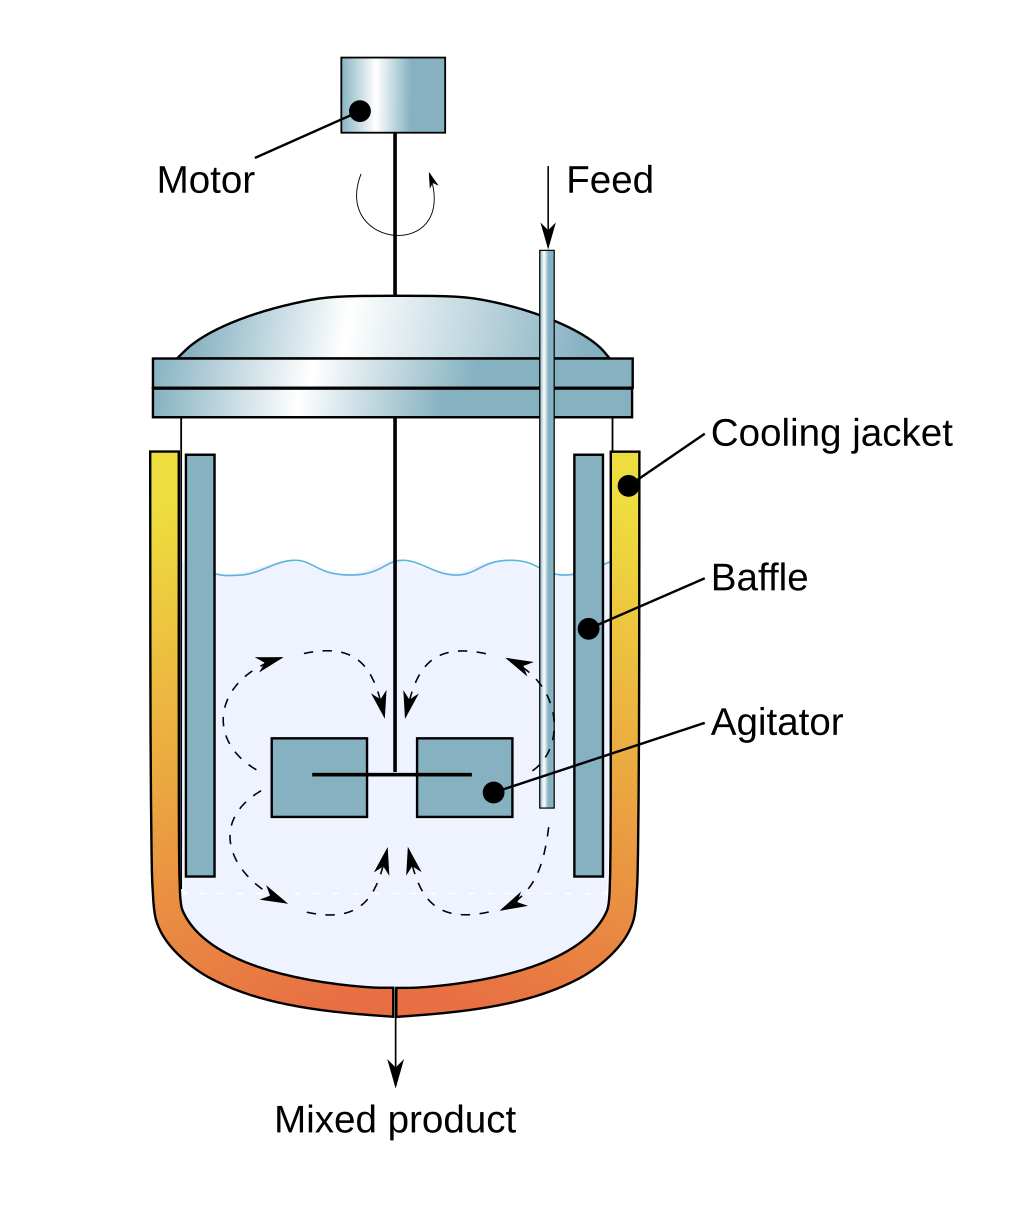
\includegraphics[width=0.3\textwidth]{02_Einfuehrung_in_Thematik/Reaktorbeispiel}
			\captionsetup{justification=centering}
			\caption{Reaktorbeispiel}
			\label{fig:Reaktorbeispiel}
		\end{figure}
		
		Der dargestellte Reaktor (\ref{fig:Reaktorbeispiel}) hat zum Beispiel folgende Funktionen:
		\begin{itemize}
			\item Befüllen
			\item Kühlen
			\item Mischen
			\item Warten
			\item Abfüllen
		\end{itemize}
		\addvspace{5mm} 
		
		Aus diesen Funktionen lassen sich verschiedene Operationen definieren, welche wiederum vom Rezept verwendet werden können, um ein bestimmtes Produkt zu prozessieren. 
		\begin{wrapfigure}{r}{0.5\textwidth}
			\centering
			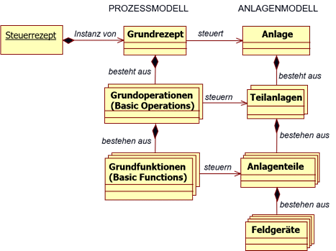
\includegraphics[width=0.5\textwidth]{02_Einfuehrung_in_Thematik/ProzessAnlageModell}
			\captionsetup{justification=centering}
			\caption{Prozess- und Anlagenmodell}
			\label{fig:ProzessAnlageModell}
		\end{wrapfigure}
		Ein zentraler Aspekt für die Flexibilität und Modularität von Chargensteuerungen nach ANSI/ISA-88 ist die Trennung von Prozessmodell und Anlagenmodell (\ref{fig:ProzessAnlageModell}). Das Prozessmodell beinhaltet das Rezept, die Operationen und Funktionen. Die Rezeptlogik ist unabhängig von den spezifischen Elementen, die in der Anlage verwendet wird. Es beschreibt lediglich, was getan werden soll, um das gewünschte Ergebnis zu erzielen, nicht wie oder mit welchen Elementen es durchgeführt wird. Das Anlagenmodel ist für das Ansteuern der Anlagenkomponenten zuständig. Die Trennung von Prozess und Anlage ermöglicht es, dass ein Rezept auf unterschiedlichen Anlagen ausgeführt werden kann. Das Rezept beschreibt, was zu tun ist, unabhängig davon, welche spezifischen Anlagenelemente verfügbar sind.
		
	\vspace{3mm}
	
	\textbf{Frage 1.3:} Wie wird eine chargenorientierte Struktur in TwinCAT umgesetzt \vspace{2mm} 
	\\
		Als Referenz für den Aufbau einer Rezeptursteuerung auf Basis von Codesys dient das Buch «Speicherprogrammierbare Steuerungen in der Industrie 4.0» von Matthias Seitz.
		\\
		Auch in TwinCAT unterscheidet man, wie beschrieben, zwischen dem Prozessmodell und dem Anlagenmodell. Das Prozessmodell beinhaltet das Rezept, die Operationen und die Funktionen. Alle werden mittels Ablaufsprache (AS) umgesetzt. Innerhalb des Anlagenmodells werden die Objektklassen für die verschiedenen Feldgeräte der Anlage definiert. Diese müssen zwingend objektorientiert aufgebaut werden. Die Objektklassen werden in der Anlage instanziiert. Die instanziierten Objekte werden verwendet, um die Schnittstelle zu den Funktionen zu bilden. 
		
		\begin{figure}[h!]
			\centering
			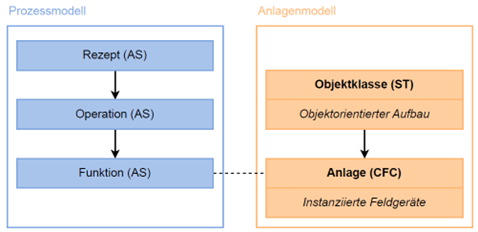
\includegraphics[width=0.7\textwidth]{02_Einfuehrung_in_Thematik/SoftwareStrukturISA88}
			\captionsetup{justification=centering}
			\caption{Softwarestruktur von ISA-88}
			\label{fig:Softwarestruktur_ISA88}
		\end{figure}
		
		Die dargestellte Struktur (\ref{fig:Softwarestruktur_ISA88}) stellt ein stark vereinfachtes Modell dar. Für eine detaillierte Beschreibung der definierten TwinCAT-Struktur, wird auf die Dokumentation des Master-Projekt 2 verwiesen.
		
	\vspace{3mm}
	
	\subsection{Grundlagenfragen für Thematik} \label{Grundlagenfragen für Thematik}
	
	\textbf{Frage 2.1:} Was versteht man unter einem skill-basierten Ansatz \vspace{2mm} 
	\\
		Ein skill-basierter Ansatz basiert auf der Fähigkeit von Maschinen bestimmte Funktionen auszuführen. Der Skill beschreibt eine konkrete Grundfunktion des Systems und stellt die tiefste Abstraktionsebene der Systemfunktion dar. Die Idee hinter dem skill-basierten Ansatz ist, dass Abläufe auf einfache Skills heruntergebrochen werden können. Durch die Verkettung von Skills, mit der Zuweisung von Funktionsparametern, können dann komplexe Funktionalitäten erstellt werden. Das Ziel dieses Ansatzes ist die Vereinfachung der Programmierung eines Systems (z.B. Roboter). In einem traditionellen, nicht-skill-basierten Ansatz würde der gesamte Prozess in einem einzigen, umfassenden Programm geschrieben werden. Das Programm würde alle Schritte in fester Reihenfolge definieren. Änderungen an einem Prozess würden dann oft bedeuten, dass das gesamte Programm geändert werden muss. Dagegen erfordern Änderungen beim skill-basierten Ansatz nur eine Änderung in der Reihenfolge oder Kombination der verwendeten Skills, nicht im gesamten Ablauf.
	\vspace{3mm}
	
	\textbf{Frage 2.2:} Vergleich zwischen einem chargenorientierten und skill-basierten Ansatz \vspace{2mm} 
	\\
		Beide Ansätze besitzen eine vergleichbare Struktur. Die Funktionalitäten eines Systems werden auf der untersten Abstraktionsstufe auf Funktionen bzw. Skills heruntergebrochen. Diese können dann verwendet werden, um komplexere Abläufe zu definieren. Beim skillbasierten Ansatz ist der Einsatz einer Rezeptur mit definierter Chargengrösse weniger sinnvoll. Die Verwendung eines Arbeitsplanes, welcher definierte Schritte vorgibt, eignet sich besser.
		Für den skill-basierten Ansatz werden für den Rahmen dieser Arbeit folgende Begriffe (\ref{fig:Softwarestrukturvergleich}) verwendet, um die verschiedenen Strukturelemente zu beschreiben. 
	
		\begin{figure}[h!]
			\centering
			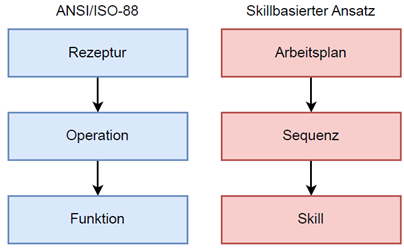
\includegraphics[width=0.4\textwidth]{02_Einfuehrung_in_Thematik/Strukturvergleich}
			\captionsetup{justification=centering}
			\caption{Softwarestrukturvergleich}
			\label{fig:Softwarestrukturvergleich}
		\end{figure}
	
	\vspace{3mm}
	
	\textbf{Frage 2.3:} Was sind die Vorteile eines skill-basierten Ansatzes \vspace{2mm} 
	\\
		Komplizierte Abläufe werden in einfache Teilfunktionen aufgeteilt. Die gesamte Funktionalität des Systems wird entsprechend innerhalb der Skills umgesetzt. Das System kann dadurch einfacher und zugänglicher programmiert werden, da diese modular und flexibel kombiniert und mit entsprechenden Parametern versehen werden können. Dies erhöht auch die Verständlichkeit des Programms für Aussenstehende oder bei nachträglichen Anpassungen. 
		Bei funktionalen Anpassungen werden nur die entsprechenden Skills bearbeitet und nicht das komplette Programm.
		\\
		\begin{wrapfigure}{l}{0.35\textwidth}
			\centering
			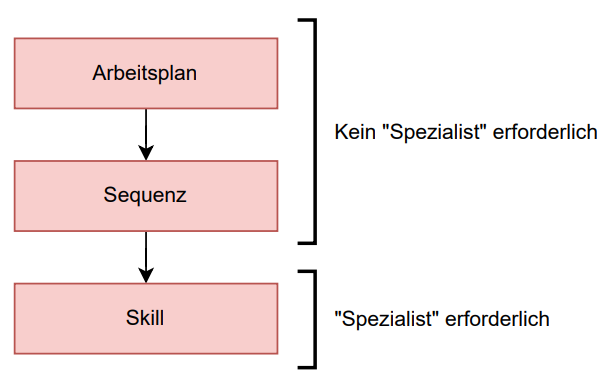
\includegraphics[width=0.35\textwidth]{02_Einfuehrung_in_Thematik/StrukturKompetenzen}
			\captionsetup{justification=centering}
			\caption{Kompetenzaufteilung}
			\label{fig:Kompetenzaufteilung}
		\end{wrapfigure}
		Da die Skills die Schnittstelle zu den Systemkomponenten darstellen, wird nur dort ein fundiertes Wissen über die Programmierung der Komponenten vorausgesetzt. Auf den oberen Stufen (Sequenz / Arbeitsplan) wird kein fundiertes Wissen über die Komponenten benötigt. Die Kompetenzen können bei einem skill-basierten Ansatz somit besser aufgeteilt werden (\ref{fig:Kompetenzaufteilung}). 
		\\
		Ein System, welches mit einem skill-basierten Ansatz programmiert wurde, ist einfach und schnell erweiterbar mit neuen Skills, wenn z.B. neue Produkte auf dem System prozessiert werden sollen. Es ist auch möglich einen Standard für die Schnittstellen der Skills zu definieren. Man beschreibt klar, welche Inputs ein Skill benötigt und welche Outputs dieser liefern muss.
		\\
		\vspace{-7mm}
		\begin{wrapfigure}{r}{0.4\textwidth}
			\centering
			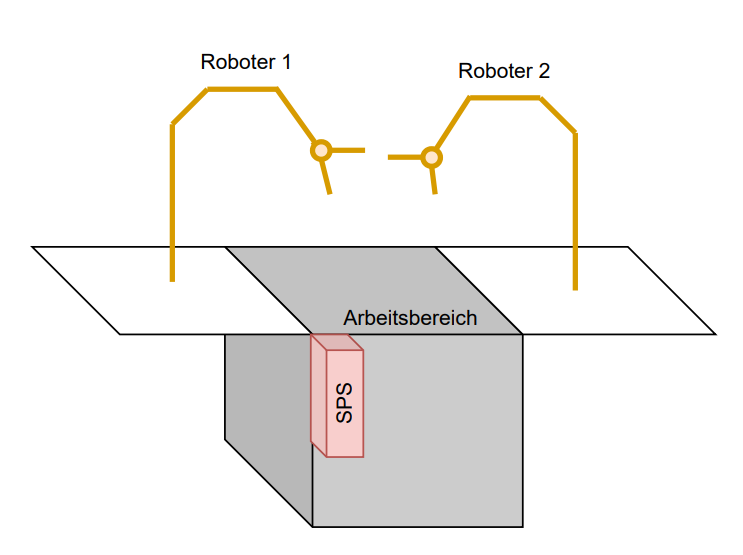
\includegraphics[width=0.4\textwidth]{02_Einfuehrung_in_Thematik/BeispielSystem}
			\captionsetup{justification=centering}
			\caption{Beispielszenario}
			\label{fig:Beispielszenario}
		\end{wrapfigure} \par
		Sequenzen und Arbeitspläne können dadurch anlagenunabhängig aufgebaut werden, da Schnittstellen immer dieselben bleiben. Somit lassen sich Prozess (Sequenzen / Arbeitspläne) bereits definieren, ohne dass die Komponenten im System bekannt sind. Dadurch können auch dynamische Anwendungen realisiert werden.Dies wird anhand einer Beispielsituation erklärt. Ein System besteht aus einem Arbeitsbereich, auf welchem Aufgabe A und B ausgeführt werden soll (\ref{fig:Beispielszenario}).  
		Zur Ausführung dieser Aufgaben besitzt das System zwei Roboter, welche über eine SPS gesteuert werden. Alle Arbeitsprozesse wurden in einzelne Skills aufgeteilt. Durch den anlagenunabhängigen Arbeitsplan kann das System selbst definieren, welcher Roboter Aufgabe A oder B ausführt. Wenn nun Roboter 1 mit Aufgabe A beschäftigt ist, kann Roboter 2 Aufgabe B ausführen oder umgekehrt. Der dynamische Prozess führt zu einer hohen Flexibilität. Roboter 1 und 2 müssen auch nicht vom selben Hersteller kommen. Sofern die Schnittstellen des Skills korrekt definiert wurden, spielt dies für den Prozess keine Rolle. 
	
	\vspace{3mm}
	
	\textbf{Frage 2.4:} Was sind die Herausforderungen eines skill-basierten Ansatzes \vspace{2mm} 
	\\
		Die grösste Herausforderung ist das Herunterbrechen der gesamten Funktionalität einer Roboteranwendung auf Skills. Eine Roboteranwendung kann sehr komplexe Prozesse realisieren, in welchen viele unterschiedliche Aktoren und Sensoren miteinander interagieren. Die umfangreichen Möglichkeiten eines solchen Systems sollen nicht durch die Verwendung von Skills eingeschränkt werden. Falls ein Standard definiert wird, müssen die Systemkomponenten die definierten Schnittstellen zur Verfügung stellen können. Dies wäre ein wichtiger Aspekt einer anlagenunabhängiger Prozessdefinierung auf Stufe der Sequenzen und Arbeitspläne. Zusätzlich soll das Arbeiten mit einem skill-basierten Ansatz nicht aufwändiger werden als das konventionelle Programmieren der Roboteranwendung. 
	\vspace{3mm}
	
	\textbf{Frage 2.5:} Wie wird eine skill-basierte Struktur in TwinCAT umgesetzt \vspace{2mm} 
	\\
		Grundsätzlich kann die Struktur aufgebaut werden wie bei einem chargenorientierten Ansatz. Man hat wieder zwei Modelle, das Prozessmodell und das Anlagemodell. Das Prozessmodell implementiert die Skills, aus welchen die Sequenzen und Arbeitspläne bestehen. Die wohl wichtigsten Elemente der Struktur sind die Objektklassen der Komponenten. Hier wird die Funktionalität der Komponenten, wie z.B. des Roboters, des Greifers aber auch des Vision-Systems programmiert. Diese können dann in der Anlage instanziiert werden. Der Skill greift auf diese instanziierten Objekte zu und führt damit einen definierten Prozess aus. 
	
		\begin{figure}[h!]
			\centering
			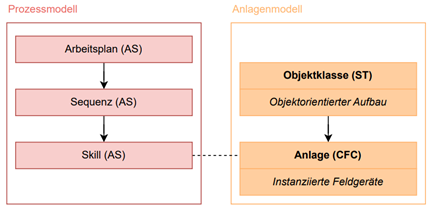
\includegraphics[width=0.7\textwidth]{02_Einfuehrung_in_Thematik/StrukturAngepasst}
			\captionsetup{justification=centering}
			\caption{Angepasste Struktur}
			\label{fig:StrukturAngepasst}
		\end{figure}
		
		Die angegebene Struktur (\ref{fig:StrukturAngepasst}) stellt eine erste Einschätzung dar, welche anhand Erfahrungen des Master-Projekt 2 gemacht wurden. Während der Erarbeitung der Thesis kann sich diese noch verändern. 
	
	\newpage
	
	\subsection{Technische Grundfragen} \label{Technische Grundfragen}
	
	\textbf{Frage 3.1:} Welche Komponenten können im System zum Einsatz kommen \vspace{2mm} 
	\\
		Ein komplettes System kann aus mehreren Aktoren und Sensoren bestehen, welche miteinander interagieren müssen, um einen bestimmten Prozess durchzuführen. Einige mögliche Komponenten werden in der folgenden Liste (\ref{tab:Komponentenliste für Roboter}) aufgezählt.
		
		\begin{table}[h!]
			\centering
			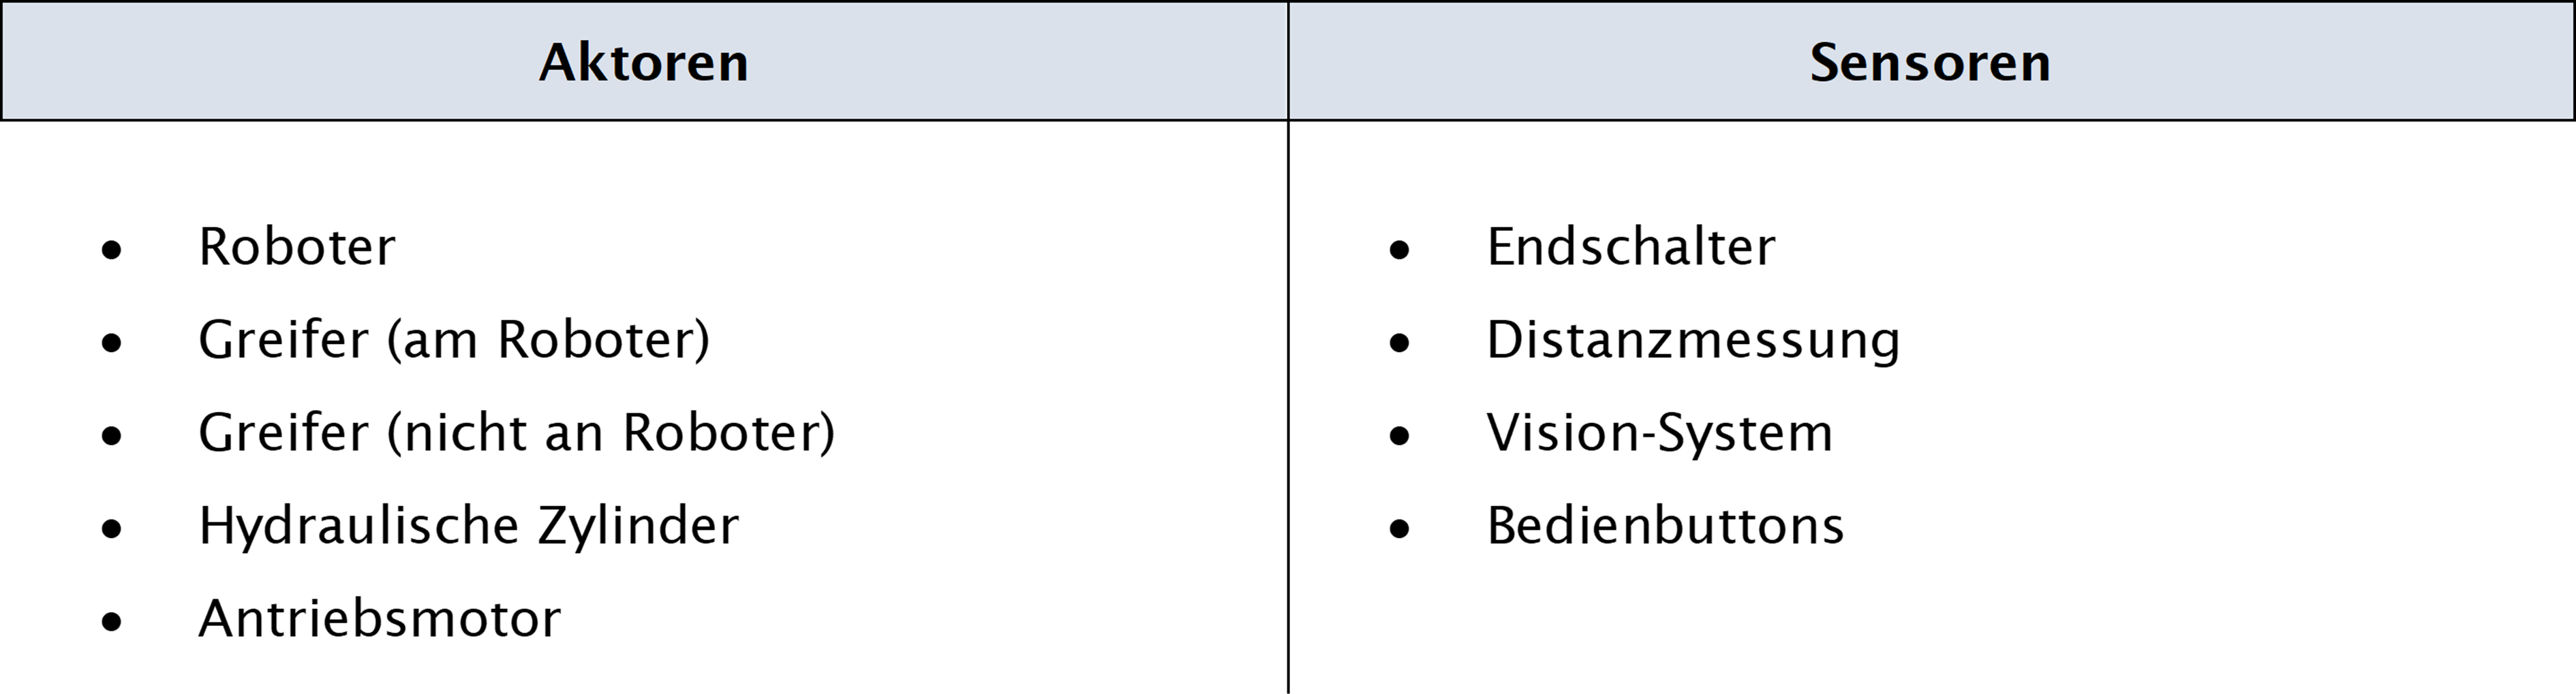
\includegraphics[width=0.8\textwidth]{02_Einfuehrung_in_Thematik/Komponentenliste}
			\captionsetup{justification=centering}
			\caption{Komponenten für Robotersystem}
			\label{tab:Komponentenliste für Roboter}
		\end{table}
		
		Alle Komponenten eines Systems müssen mit der SPS interagieren können und haben einen Einfluss auf den Prozess. Die wohl aufwändigste Schnittstelle ist die SPS-Roboter-Schnittstelle. Fast alle anderen Komponenten können über entsprechende Beckhoff-Klemmen in die SPS integriert werden.
	
	\vspace{3mm}
	
	\textbf{Frage 3.2:} Welche Roboter stehen zur Verfügung \vspace{2mm} 
	\\
		Um eine grosse Bandbreite an Möglichkeiten für das System zu haben, soll für das Projekt ein 6-Achs-Roboter eingesetzt werden. Damit der zeitliche Rahmen der Thesis voll genutzt werden kann, werden Roboter betrachtet, welche im Moment an der BFH, im Bereich der Maschinentechnik, zur Verfügung stehen (\ref{tab:Robotervergleich}). 
		
		\begin{table}[h!]
			\centering
			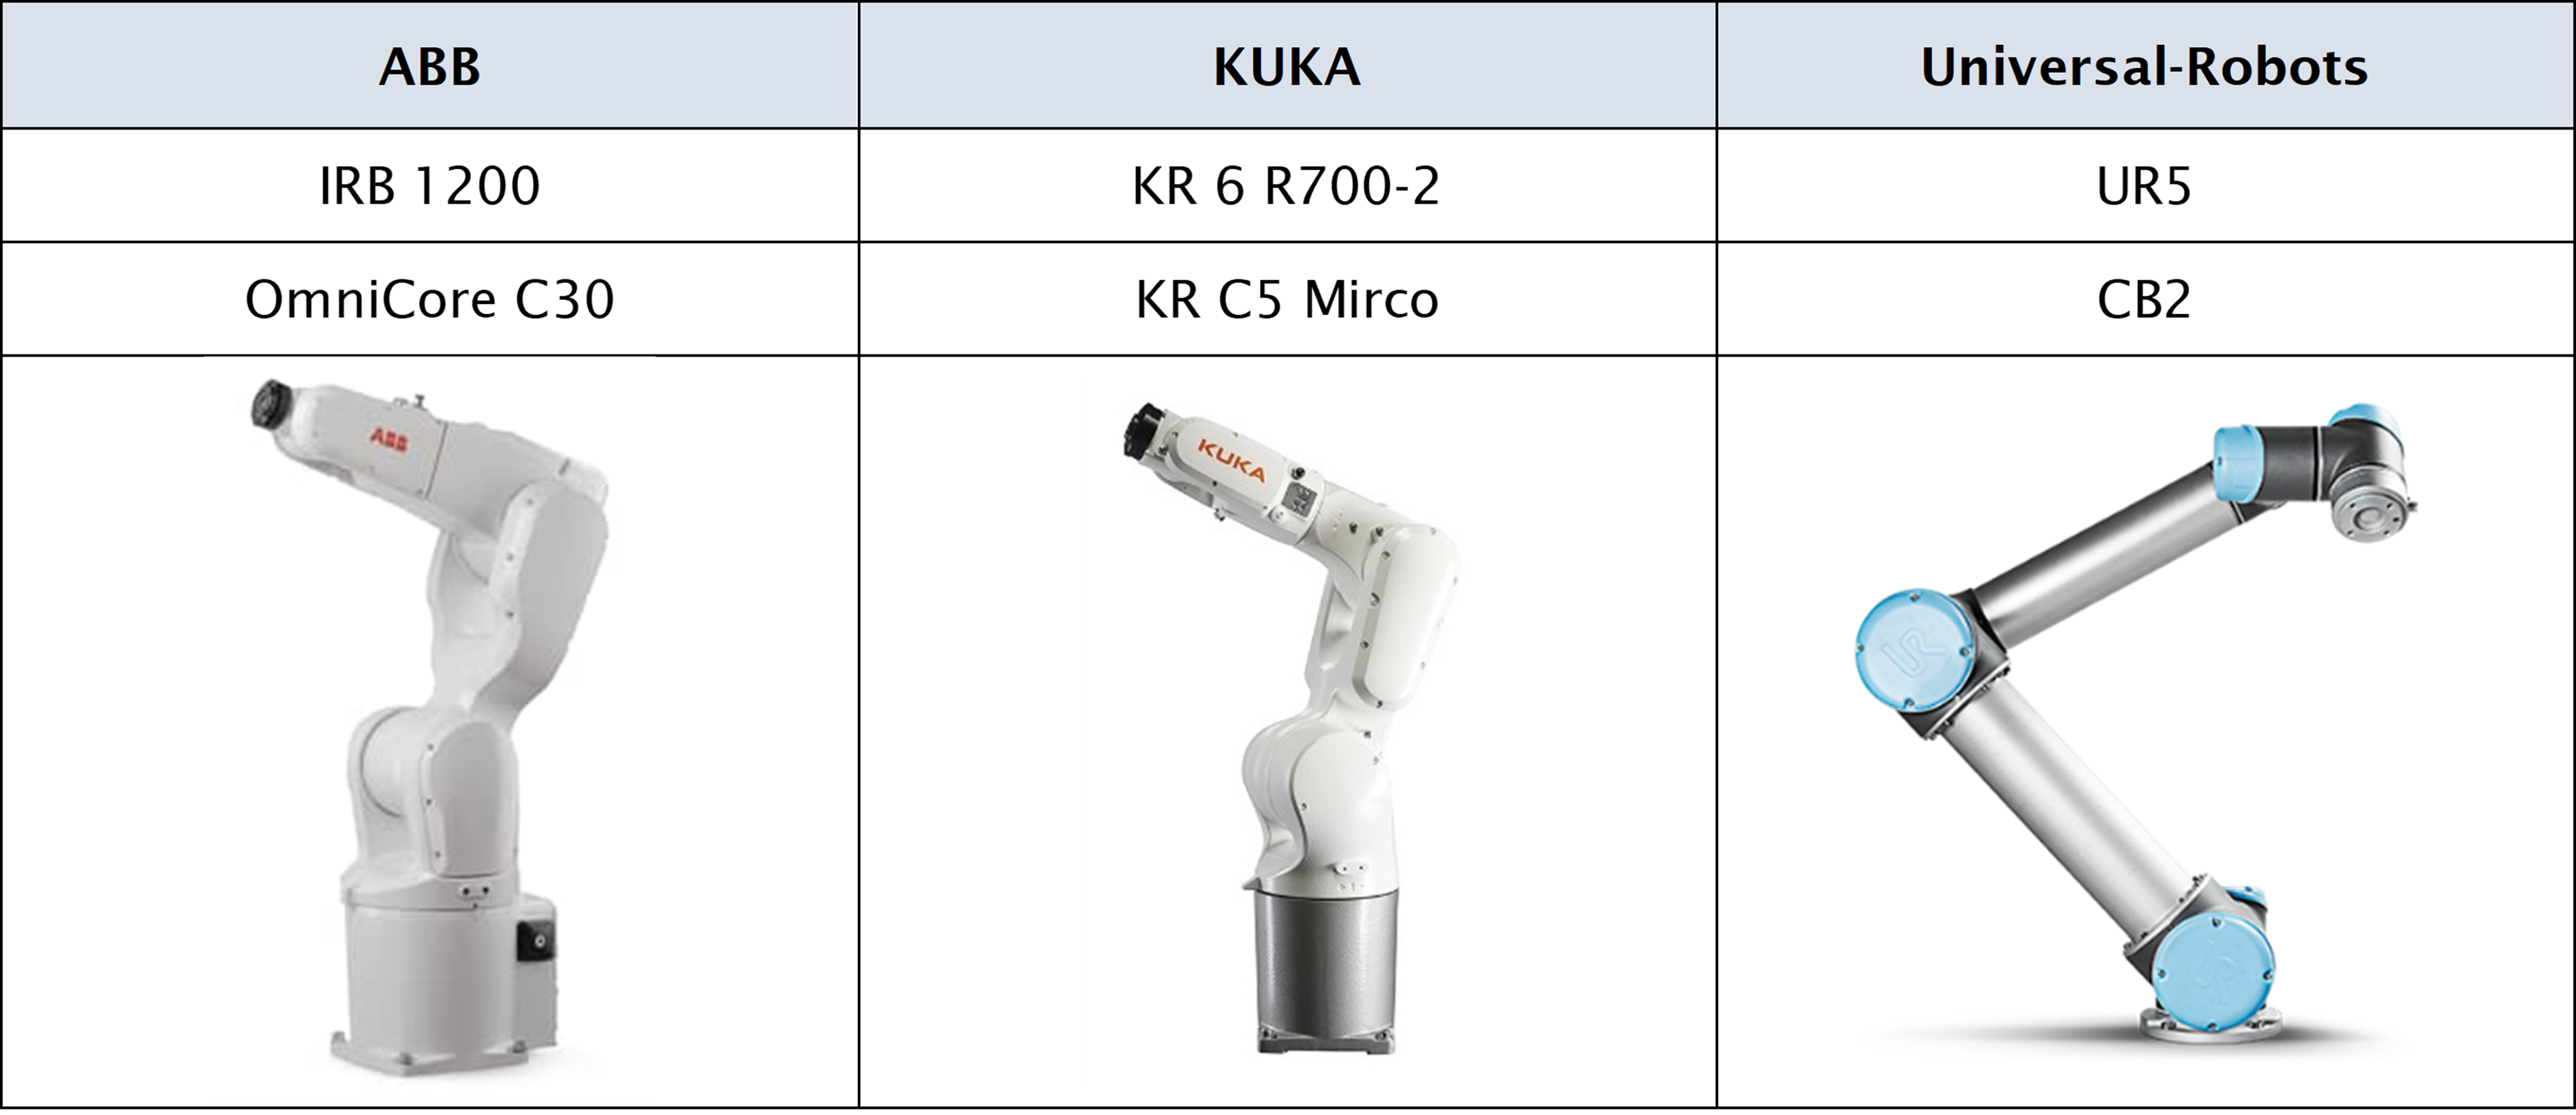
\includegraphics[width=1\textwidth]{02_Einfuehrung_in_Thematik/Robotervergleich}
			\captionsetup{justification=centering}
			\caption{Gegenüberstellung der Roboter}
			\label{tab:Robotervergleich}
		\end{table}
	\vspace{3mm}
	
	\newpage
	
	\textbf{Frage 3.3:} Welche Schnittstellen bieten die Roboter zu einer SPS \vspace{2mm} 
	\\
		Innerhalb dieser Analyse werden die Möglichkeiten aufgelistet, wie die SPS mit dem Roboter verbunden werden könnte. Details über die Kommunikationsschnittstelle oder die benötigten Hersteller-Tools werden bei der Erarbeitung weiter ausgeführt.  
		\vspace{3mm}
		
		ABB (IRB 1200 / OmniCore C30):
		\vspace{2mm}
		\\
		Für die direkte Steuerung eines Roboters kann EGM (Glossar) von ABB verwendet werden.   Mit EGM können Befehle via RAPID-Tasks an den Controller gesendet werden und es können Daten empfangen werden. Die Kommunikation wird über eine UdpUc-Schnittstelle realisiert (\ref{fig:ABB_EGM}). 
		
		\begin{figure}[h!]
			\centering
			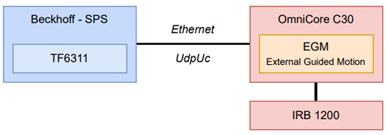
\includegraphics[width=0.5\textwidth]{02_Einfuehrung_in_Thematik/ABB_EGM}
			\captionsetup{justification=centering}
			\caption{ABB-Schnittstelle über EGM}
			\label{fig:ABB_EGM}
		\end{figure}
		
		Es ist auch möglich den Roboter mit OPC UA- oder TCP/IP-Schnittstellen anzusprechen. Hierbei kann jedoch nicht direkt mit dem Roboter kommuniziert werden. Die Verbindung zwischen SPS und Controller wird über RobotStudio von ABB hergestellt. In RobotStudio muss ein Programm laufen, welches die Schnittstellen-Variablen auswertet und interpretiert. Für die OPC-UA-Schnittstelle wird auf der SPS der OPC-UA-Server eingerichtet. RobotStudio dient als Client (\ref{fig:ABB_OPC}).
		
		\begin{figure}[h!]
			\centering
			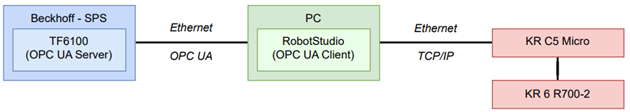
\includegraphics[width=0.9\textwidth]{02_Einfuehrung_in_Thematik/ABB_OPC}
			\caption{ABB-Schnittstelle über OPC}
			\label{fig:ABB_OPC}
		\end{figure}
		\vspace{3mm}
		
		KUKA (KR 6 R700-2 / Kr C5 Mirco):
		\vspace{2mm}
		\\
		Mit «KUKA.PLC mx Automation» bietet KUKA eine standardisierte Schnittstelle zwischen der Robotersteuerung und der SPS. Dies erlaubt es, den Roboter vollständig durch die SPS in Echtzeit zu steuern. Dafür werden Funktionsbausteine zur Verfügung gestellt, welche in der SPS verwendet werden können. Um auf diese zugreifen zu können, muss das Beckhoff-Paket TF5120 (TwinCAT 3 Robotics mxAutomation) installiert werden (\ref{fig:KUKA_mxA}). Eine komplette Liste der Funktionen ist im entsprechenden Beckhoff-Handbuch aufgeführt.
		
		\begin{figure}[h!]
			\centering
			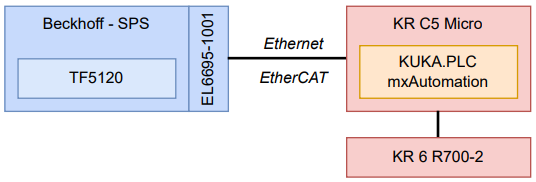
\includegraphics[width=0.5\textwidth]{02_Einfuehrung_in_Thematik/KUKA_MxA}
			\captionsetup{justification=centering}
			\caption{KUKA-Schnittstelle über mxAutomation}
			\label{fig:KUKA_mxA}
		\end{figure}
		
		\newpage
		
		Damit der Kontroller und die SPS miteinander kommunizieren können, wird eine spezielle EtherCAT-Klemme (EL6695-1001) benötigt, welche von KUKA angeboten wird. 
		\\
		Auch eine Schnittstelle über OPC UA ist möglich. Jedoch dient hierbei der Controller als OPC-UA-Server und definiert Kommunikationsvariablen. Die SPS wird als Client eingesetzt. Der Roboter könnte über diese Schnittstelle nur gesteuert werden, wenn auf dem Controller Programme ausgeführt werden, welche die Kommunikationsvariablen auswerten und entsprechende Aktionen auslösen. 
		\vspace{3mm}
		
		Universal-Robots (UR5 / CB2):
		\vspace{2mm}
		\\
		Über eine TCP/IP-Schnittstelle kann die SPS mit dem Controller von Universal Robots kommunizieren. Für eine solche Kommunikationsschnittstelle muss das Beckhoff-Paket TF6310 (TwinCAT 3 TCP/IP) installiert werden (\ref{fig:UR_TCPIP}). Über die von Universal Robots entwickelte Programmiersprache URScript kann der Roboter programmiert werden. URScript ermöglich eine ausführliche Kontrolle über den Roboter.
		
		\begin{figure}[h!]
			\centering
			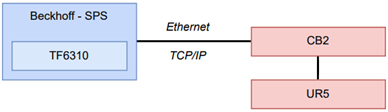
\includegraphics[width=0.6\textwidth]{02_Einfuehrung_in_Thematik/UR5_TCPIP}
			\captionsetup{justification=centering}
			\caption{UR-Schnittstelle über TCP/IP}
			\label{fig:UR_TCPIP}
		\end{figure}
	
	\vspace{3mm}
	
	\newpage
	
	\textbf{Frage 3.4:} Was sind die Anwendungen eines Roboters in der Industrie \vspace{2mm} 
	\\
		Das folgende Mindmap (\ref{fig:Roboteranwendung}) zeigt einen groben Umriss von Anwendungen für einen Roboter in der Industrie. Es wird nicht zwischen kollaborativen und industriellen Roboter unterschieden. 
		
		\begin{figure}[h!]
			\centering
			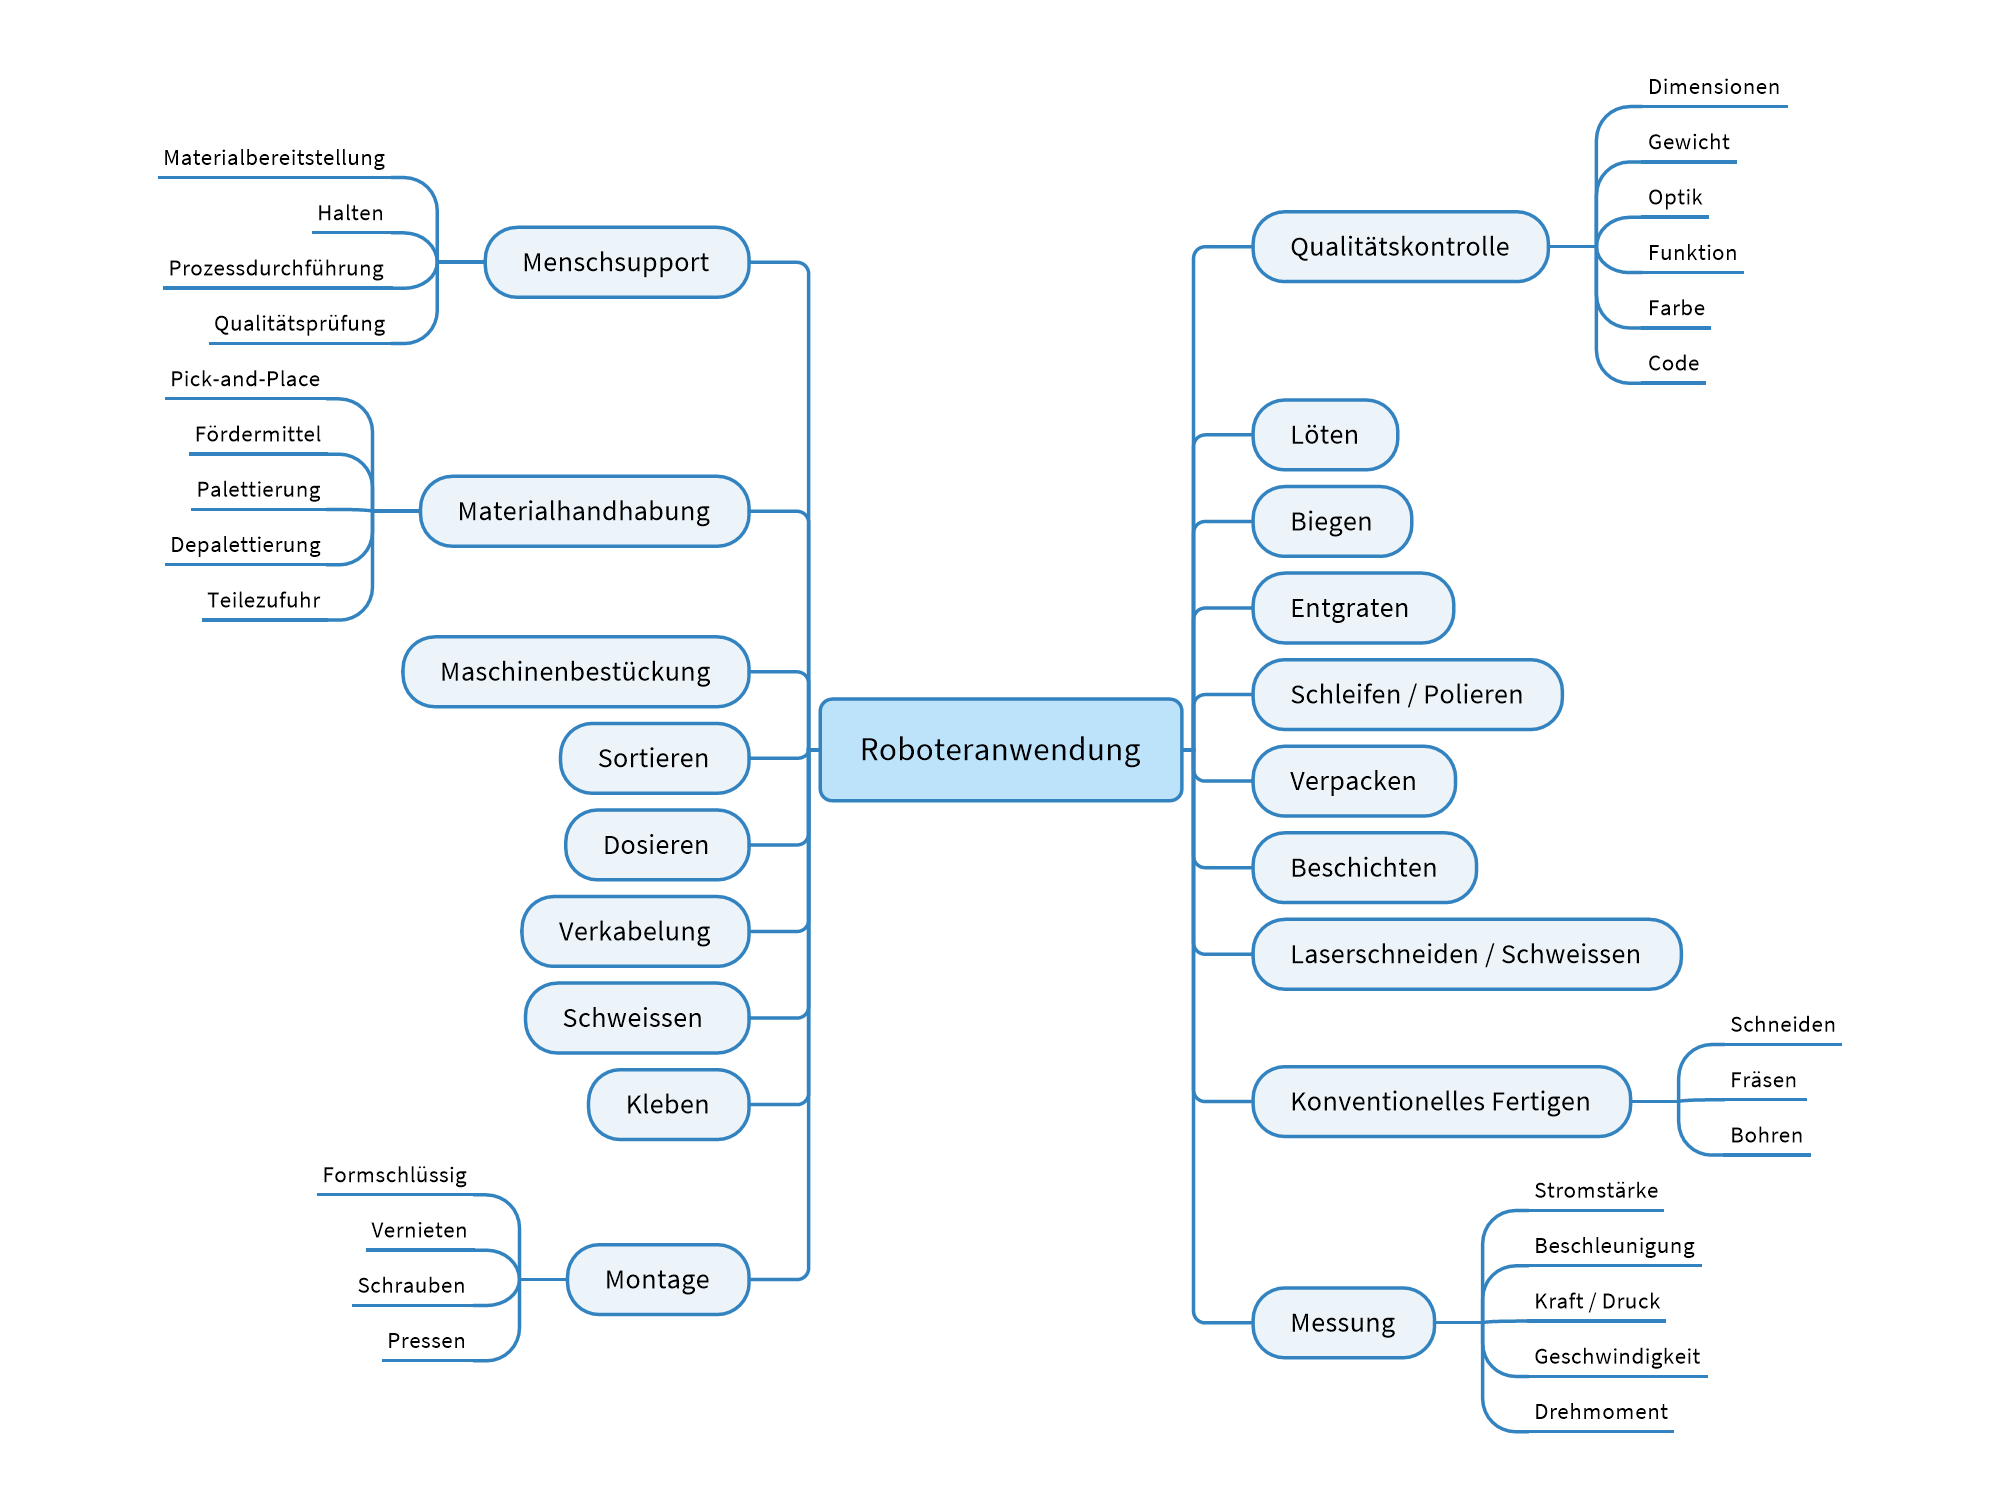
\includegraphics[width=1\textwidth]{02_Einfuehrung_in_Thematik/Roboteranwendung}
			\captionsetup{justification=centering}
			\caption{Roboteranwendung}
			\label{fig:Roboteranwendung}
		\end{figure}
		
		Ein skill-basierter Ansatz eignet sich besonders für Aufgaben, bei denen Anpassungen am Ablauf erforderlich sind, wie beispielsweise bei der Positionierung oder Ausrichtung eines Objekts. Mit diesem Ansatz kann flexibel auf unterschiedliche Situationen reagiert werden. Das traditionelle Teach-In-Verfahren ist hingegen effizienter für Prozesse, die wiederholte und unveränderte Roboterbewegungen erfordern.
		\\
		Während sich ein skill-basierter Ansatz grundsätzlich für viele Anwendungen eignet, entfaltet er seinen Vorteil besonders in Szenarien mit variierenden Bedingungen. Werden hingegen immer dieselben Bauteile verarbeitet, ist das klassische Verfahren oft die bessere Wahl. Bei wechselnden Bauteilen hingegen bietet der skill-basierte Ansatz einen klaren Mehrwert.
		
		
	\vspace{3mm}

	\newpage


\section{Marktanalyse} \label{Marktanalyse}

	\textbf{Frage 1:} Wurden bereits vergleichbare Projekte und Ansätze durchgeführt \vspace{2mm} 
	\\
	
	Referenzprojekt 1:
	\vspace{2mm}
	\\
	\begin{tabularx}{\textwidth}{@{}>{}p{8em} X@{}}
		Rahmen: & 
		MSE-Master-Thesis an der BFH
		\\
		
		Titel: & 
		Skill-basierte Aufgabenplanung für Roboter in Handarbeitsplätzen von Herstellungs-prozessen 
		\\
		
		Beschreibung: & 
		Innerhalb der Master-Thesis wurde für die Firma Ypsomed AG eine spezifische Anwendung mit skill-basierter Aufgabenplanung umgesetzt. Das Ziel dieser Arbeit war eine Roboterlösung zu entwickeln, die einen raschen Einsatz eines Roboters in der Produktion zum Automatisieren verschiedener und wechselnder Aufgaben ermöglicht. Dafür wurden die Teilaufgaben durch parametrierbare Skills umgesetzt, wodurch komplexe Prozessabläufe abgebildet werden konnten.
		
		Das Projekt verwendete einen UR5e-Roboter in Kombination mit einem Greifer und einem Vision-System. Als wichtiges Softwareframework wurde ROS eingesetzt. Jedoch gab es noch weitere Software-Komponenten, welche für das Projekt eingesetzt wurden und miteinander interagiert haben. Das Projekt setzte sich mit Themen wie Lokalisieren der Objekte, das Berechnen des Griffs und das Planen des Roboterablaufs auseinander.
		
		Die Grundfunktionalitäten, welche sich aus der vorgegebenen Anwendung der Firma Ypsomed AG ergaben, wurden als Skills umgesetzt. Die Logik des Skills wurde als Zustandsmaschine aufgebaut. 
		
		Der umgesetzte Prototyp funktionierte für die definierte Anwendung. Einige Funktionalitäten wurden jedoch noch nicht ganz umgesetzt und die Ausführungszeiten des Prozesses sind höher als bei einer händischen Durchführung. 
		\\
		
		Erkenntnisse: & 
		\begin{itemize}
			\item Allgemeine Idee des skill-basierten Ansatzes hat funktioniert
			\item Könnte als Referenz für mögliche Skill-Definition dienen (Parameter/Variablen)
			\item Die umgesetzte Lösung könnte auch mit einer SPS-Schnittstelle betrieben werden
			\item Thematik der Trennung zwischen Prozess und Anlage wurde als zukünftiger Schritt definiert. Im Moment ist die Struktur anlagenspezifisch.
			\item Die umgesetzte Lösung setzt auf viele unterschiedliche Software-Tools mit entsprechenden Schnittstellen
		\end{itemize}
	\end{tabularx}
	
	\newpage
	
	Referenzprojekt 2:
	\vspace{2mm}
	\\
	\begin{tabularx}{\textwidth}{@{}>{}p{8em} X@{}}
		Rahmen: & 
		International Conference on Intelligent Robots and Systems (IROS)
		\\
		
		Titel: & 
		SkiROS2: A skill-based Robot Control Platform for ROS 
		\\
		
		Beschreibung: & 
		Das Dokument beschreibt SkiROS2, welches eine skill-basierte Robotersteuerungsplattform auf Basis von ROS darstellt.  Die Struktur wurde darauf ausgelegt, kleine Batchgrössen, welche komplexe Abläufe benötigen, umzusetzen.  Die Architektur von SkiROS2 besteht aus einem Skill Manager und einem World Model, welche das Kernsystem bilden.
		
		Mit dieser Struktur ist es möglich, mehrere Roboter zu steuern und miteinander zu synchronisieren. Das World Model speichert Instanzen der aktuellen Situation. Es enthält semantische Informationen über Roboter, Objekte und Orte und bietet eine API für das Lesen und Schreiben von Daten. Es kann zur Planung und Parametrisierung von Skills genutzt werden. Jeder Roboter hat einen eigenen Skill Manager, der Skills aus Bibliotheken lädt, diese initialisiert und überwacht. Er übernimmt auch die Ausführung und teilt Aufgaben eindeutig zu.
		
		Alle Skills besitzen die gleiche Struktur. Die Skill-Schnittstelle definiert die benötigten Parameter, wie auch die Pre-, Hold- und Post-Bedingung. Diese werden als Transitionen verwendet, welche den Skill starten, beenden oder abbrechen. Es wird zwischen zwei Skill-Arten unterschieden. Die «primitive» Skills sind Aktionen, welche vom System in der realen Welt ausgeführt werden (z.B. Greifen). Diese haben drei Zustände: «running», «success» und «failure». Die «compound» Skills stellen einen Zusammenschluss von «primitive» oder «compound» Skills dar und sind durch einen Ablauf definiert. 
		
		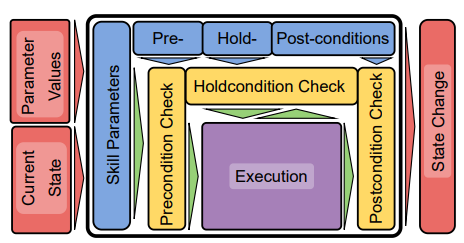
\includegraphics[width=1\linewidth]{02_Einfuehrung_in_Thematik/SkiROS2_Skill}
		\\
		
		Erkenntnisse: & 
		\begin{itemize}
			\item SkiROS2 scheint eine bereits sehr ausgereifte Umsetzung eines skill-basierten Ansatzes zu sein 
			\item Ein Grundwissen über ROS, der allgemeinen Struktur von SkiROS2 und das Programmieren in Python ist erforderlich, um es einsetzen zu können
			\item Ansätze der Strukturierung können als Referenz für Thesis dienen
		\end{itemize}
	\end{tabularx}
	
	\newpage
	
	Referenzprojekt 3:
	\vspace{2mm}
	\\
	\begin{tabularx}{\textwidth}{@{}>{}p{8em} X@{}}
		Rahmen: & 
		Dissertation an der Universität Stuttgart 
		\\
		
		Titel: & 
		Prototypbasiertes Skill-Modell zur Programmierung von Robotern für kraftgeregelte Montageprozess
		\\
		
		Beschreibung: & 
		Die Arbeit zielt darauf ab, den Einsatz von Industrierobotern in Montageanwendungen zu erleichtern, indem ein skill-basierter Ansatz zur Programmierung von kraftgeregelten Montageprozesse entwickelt wurde. 
		
		Innerhalb der Arbeit wurde das komplette System entworfen. Die Skills werden in Bereich Koordination gehandhabt.  
		
		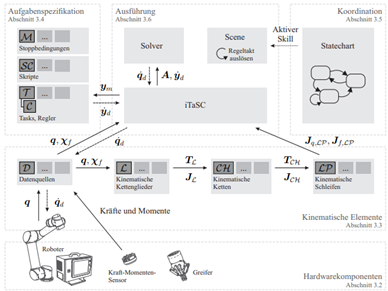
\includegraphics[width=1\linewidth]{02_Einfuehrung_in_Thematik/Disseration_Struktur}
		
		Für das Projekt wurde ein eigenes Skill-Modell entworfen, mit dem Namen «pitasc»
		Das entwickelte Skill-Modell basiert auf drei Grundpfeilern: Abstraktion, Komposition und Vererbung. Hierbei wird eigentlich das Herunterbrechen der Funktionen des Systems auf anlagenunabhängige Parameter beschrieben. 
		
		Die Arbeit wurde für das Fraunhofer-Institut für Produktionstechnik und Automatisierung erstellt. Das Institut bietet den pitasc-Systembaukasten mittlerweile zum Kauf an. 
		\\
		
		Erkenntnisse: & 
		\begin{itemize}
			\item Das pitasc-Skill-Modell könnte für das Projekt spannend sein
			\item Die Thematik der Positions-, Geschwindigkeits- und Kraftregelung kann ein relevanter Punkt werden (z.B. Aufstecken von Klemme auf DIN-Schiene). Die iTaSC-Formulierung könnte dafür hilfreich sein. 
			\item Das entworfene Skill-Modell ist anlagenunabhängig. 
			\item Die Software macht einen sehr komplexen Eindruck, was sich wahrscheinlich in der Anwendung und Bedienung widerspiegelt.
			\item Das beschriebene System beinhaltet kein Vision-System
		\end{itemize}
	\end{tabularx}
	
		\newpage
	
	Referenzprojekt 4:
	\vspace{2mm}
	\\
		\begin{tabularx}{\textwidth}{@{}>{}p{8em} X@{}}
		Rahmen: & 
		Research-Paper des Fraunhofer-Institut für Werkzeugmaschinen und Umformtechnik 
		\\
		
		Titel: & 
		Flexible skill-based control for robot cells in manufacturing
		\\
		
		Beschreibung: & 
		Das Forschungsprojekt stellt die Methode zur Programmierung flexibler, auf Skills basierender Steuerungen für Roboteranwendung vor. Dabei wird stark auf die Vorteile einer solchen Methode eingegangen. Als Hauptvorteil wird die Fähigkeit angegeben, dass der Prozessablauf von Bedienern angepasst und erweitert werden kann, ohne den Steuerungscode zu ändern. Für Entwicklung der Methode wurden vier Anforderungen gestellt: Erweiterbarkeit, Flexible Nutzbarkeit, Konfigurierbarkeit und Wiederverwendbarkeit. Um diese Anforderungen zu erfüllen, wurde die «skill-based control architecture (SBC)» angewendet, welche im Dokument «Evaluating Skill-Based Control Architecture for Flexible Automation Systems» von Kirill Dorofeev und Monika Wenger beschrieben wird. 
		
		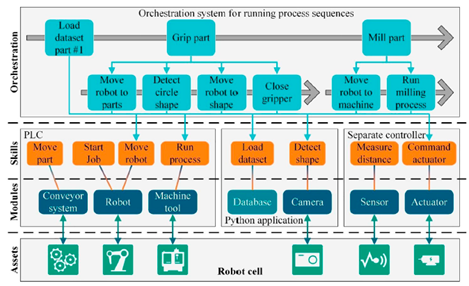
\includegraphics[width=0.8\linewidth]{02_Einfuehrung_in_Thematik/SBC}
		
		Es wird auch darauf hingewiesen, dass es bereits Richtlinien für die Standardisierung von Skills (VDI/VDE/NAMUR 2658) des VDI gibt. Wichtige Begriffe dieser Richtlinie sind PEA (Schnittstellen modularer Prozesseinheiten) und MTP (Module Type Package).
		
		Innerhalb des Projektes wurde ein Prototyp auf Basis von TwinCAT umgesetzt (inkl. HMI). Ein interessanter Aspekt des Systems ist die TwinCAT-Hot-Connect-Funktionalität. Damit können Anlagenkomponenten während des Betriebs entfernt oder hinzugefügt werden. Dies kann für das Wechseln von Greifer während dem Betrieb relevant sein. 
		
		Das Projekt hat gezeigt, dass ein Aufbau mit der SBC-Struktur aufgebaut werden kann und funktioniert. Als weiterführende Arbeiten wurde definiert, dass das benötigte Wissen zur Anwendung von skill-basierten Ansätzen weiter verringert werden muss und das dabei das HMI eine wichtige Rolle spielt. 
		\\
		
		Erkenntnisse: & 
		\begin{itemize}
			\item Das Projekt zeigt, dass eine solche Anwendung auf Basis von TwinCAT umgesetzt werden kann
			\item Das entwickelte HMI kann als Referenz für die Thesis dienen
			\item Die TwinCAT-Hot-Connect-Funktionalität kann für das Projekt relevant sein
			\item Die Richtlinie des VDI kann für das Projekt relevant sein
		\end{itemize}
	\end{tabularx}
	
	\newpage
	
	Die Analyse verdeutlicht, dass bereits zahlreiche Projekte zu diesem Thema durchgeführt wurden, die unterschiedliche Ansätze verfolgen. Diese reichen von reinen Forschungsprojekten bis hin zu Lösungen, die direkt in der Industrie Anwendung finden. Ein skill-basierter Ansatz gewinnt aufgrund neuer und spezifischer Anforderungen der Industrie zunehmend an Bedeutung.
	Die Implementierung eines vollständig skill-basierten Systems umfasst viele unterschiedliche Aspekte, wobei die gewählte Struktur eine zentrale Rolle spielt. Es gibt jedoch zahlreiche Punkte, die für diese Arbeit als Referenz dienen und im Vorfeld geklärt werden müssen. Der Umfang des Themas verdeutlicht, wie wichtig es ist, die Anforderungen an das System präzise zu definieren.
	Keines der analysierten Projekte hat die ISA-88-Norm als Grundlage für seine Struktur verwendet. Die Anwendung dieser Norm auf ein skill-basiertes System stellt daher eine innovative Herangehensweise dar.
	\vspace{3mm}
	
	\textbf{Frage 2:} Was beschreibt die Richtlinie VDI/VDE/NAMUR 2658 \vspace{2mm} 
	\\
	Die Richtlinie beschreibt das Engineering der Automatisierungstechnik modularer Anlagen, insbesondere in der Verfahrenstechnik. Sie behandelt sowohl das Modulengineering als auch das Anlagenengineering. Das Module Type Package (MTP) dient zur Definition und Beschreibung der Schnittstellen und Funktionen der Module, was die Integration in eine Prozessführungsebene ermöglicht. Die Schwerpunkte der Richtlinie umfassen:
	\begin{itemize}
		\item Allgemeines Konzept des modularen Anlagenengineerings
		\item Zustands- und Dienstmodelle modularer Anlagen
		\item Aufbau und Struktur des MTP
		\item Schnittstellen zwischen den Moduldiensten und der Prozessführungsebene (PFE)
		\item Definition des MTP-Manifests und der Kommunikationsschnittstellen (z. B. OPC UA)
		\item Modellierungsvorgaben zur Erstellung des MTP-Manifests und der Kommunikationsbeschreibung.
	\end{itemize}
	Ziel der Richtlinie ist, die Integration von Feldgeräten zu vereinfachen, damit sie effizient mit anderen Systemen zusammenarbeiten. Die Richtlinie stellt sicher, dass die Geräte herstellerunabhängig funktionieren und Daten, wie Mess- oder Diagnosedaten, standardisiert ausgetauscht werden können. Dabei werden nicht nur die Integration in Planungs- und Engineering-Software, sondern auch der Betrieb in Prozessleitsystemen sowie der gesamte Lebenszyklus der Geräte, von der Planung über den Betrieb bis zur Wartung, berücksichtigt. Dadurch können Fehler reduziert und der Aufwand für Inbetriebnahme und Wartung minimiert werden.
	\vspace{3mm}
	
	\newpage
	
	\textbf{Frage 3:} Was ist MTP \vspace{2mm} 
	\\
	MTP steht für Module Type Package und definiert standardisierte Schnittstellen zwischen Anlagenmodulen. Innerhalb eines Systems gibt es verschiedene Module, welche für eine spezielle Prozessfunktion zuständig sind. Dieses Modul wird als Functional Equipment Assembly (FEA) bezeichnet und bildet ein eigenes, geschlossenes System mit Schnittstellen gegen aussen und innen.
	\\
	\begin{figure}[h!]
		\centering
		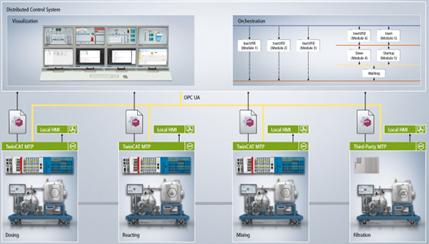
\includegraphics[width=0.8\textwidth]{02_Einfuehrung_in_Thematik/MTP}
		\captionsetup{justification=centering}
		\caption{MTP-Strukur von Beckhoff}
		\label{fig:MTP}
	\end{figure}
	\\
	Ein System besteht aus mindestens einem FEA und bildet das Process Equipment Assembly (PEA). Innerhalb des PEA können FEA entfernt oder hinzugefügt werden. Das MTP definiert eine einfache Konfiguration und Implementation der Anlagenmodule. MTPs definieren die Eigenschaften und Schnittstellen dieser Module. Das Prozessleitsystem liest die MTPs und nutzt diese, um einen Prozessablauf an die Anlagenmodule zu delegieren. Die gesamte Anlage ist dadurch flexibel einsetz- und erweiterbar.
	\\  
	Das MTP-Prinzip wird bis jetzt hauptsächlich in der Verfahrenstechnik eingesetzt. Unternehmen wie Beckhoff, ABB oder Siemens bieten MTP-Pakete für Ihre Systeme an (\ref{fig:MTP}). 
	\\
	Die standardisierte Schnittstellendefinition könnte als Referenz für die Thesis verwendet werden. Jedoch muss die Richtlinie (VDI/VDE/NAMUR 2658) gekauft werden und steht im Moment nicht zur Verfügung. 
	\vspace{3mm}
	
	\textbf{Frage 4:} Was ist der PLCopen-Standard  \vspace{2mm} 
	\\
	Der PLCopen-Standard ist eine internationale Initiative zur Standardisierung von Programmiersprachen und Funktionen einer SPS. Ziel von PLCopen ist es, die Programmierung, Entwicklung und Wartung von Steuerungssystemen zu vereinfachen und zu vereinheitlichen, um die Kompatibilität zwischen verschiedenen SPS-Systemen und Herstellern zu verbessern. Der PLCopen-Standard ergänzt die Norm IEC 61131-3, indem Bibliotheken, Modelle und Richtlinien zur Verfügung gestellt werden, die auf diesen Normen basieren und die Programmierung einer SPS noch effizienter gestalten.
	\\
	Die Richtlinie gibt einen Ansatz vor, wie Funktionsbausteine aufgebaut werden können und funktionieren. Dabei wird zwischen zwei Arten von Funktionsbausteinen unterschieden. Der pegelgesteuerte Funktionsbaustein bleibt aktive, so lange das Triggersignal aktiv ist. Der flankengesteuerte Funktionsbaustein wird bei einer Flanke aktiv und bleibt aktiv. Die Basisdefinition (\ref{fig:PLCopen_FB}) dieser Funktionsbausteine sieht wie folgt aus: 
	
	\newpage
	
	\begin{figure}[h!]
		\centering
		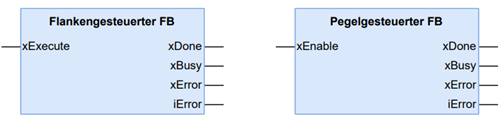
\includegraphics[width=0.8\textwidth]{02_Einfuehrung_in_Thematik/PLCopen_FB}
		\captionsetup{justification=centering}
		\caption{PLCopen-Basisfunktionsblock}
		\label{fig:PLCopen_FB}
	\end{figure}
	
	Diese Basisdefinition kann beliebig erweitert werden, z.B. mit einer Abort-Funktionalität. Das Verhalten der Funktionsbausteine wird anhand des aufgeführten Diagramms (\ref{fig:PLCopen_Ablauf}) erklärt. Die Variable «eState» gibt dabei den momentanen Zustand des Funktionsbausteins als Eigenschaft wieder.
	Der Ansatz der Funktionsbausteindefinition kann für gewisse Aspekte der Thesis relevant sein. Falls Skills als Funktionsbausteine definiert werden, könnte diese Definition helfen, diese übersichtlich und gleich zu strukturieren. 
	
	\begin{figure}[h!]
		\centering
		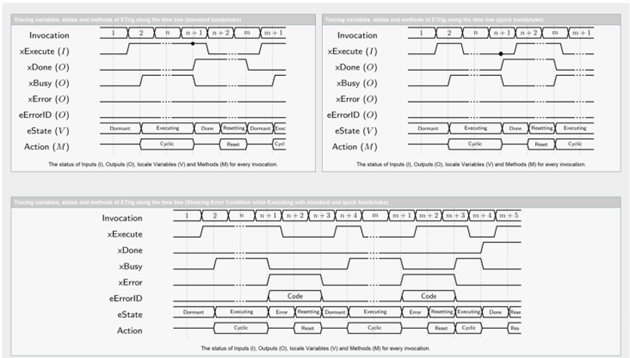
\includegraphics[width=1\textwidth]{02_Einfuehrung_in_Thematik/PLCopen_Ablauf}
		\captionsetup{justification=centering}
		\caption{PLCopen-Basisablauf}
		\label{fig:PLCopen_Ablauf}
	\end{figure}
	
	\newpage
	
	
	
\section{System- und Kontextgrenze} \label{SystemKontextGrenze}

Über die System- und Kontextgrenzen (Abb. \ref{fig:SystemKontextGrenze}) wird der Rahmen für das Projekt gesetzt. Man unterscheidet zwischen System (\textit{kann beeinflusst werden}), Systemkontext (\textit{ist relevant für das Projekt, jedoch können solche Aspekte nicht beeinflusst werden}) und irrelevanter Umgebung (\textit{spielt zum jetzigen Zeitpunkt keine Rolle}).

\begin{figure}[h!]
	\centering
	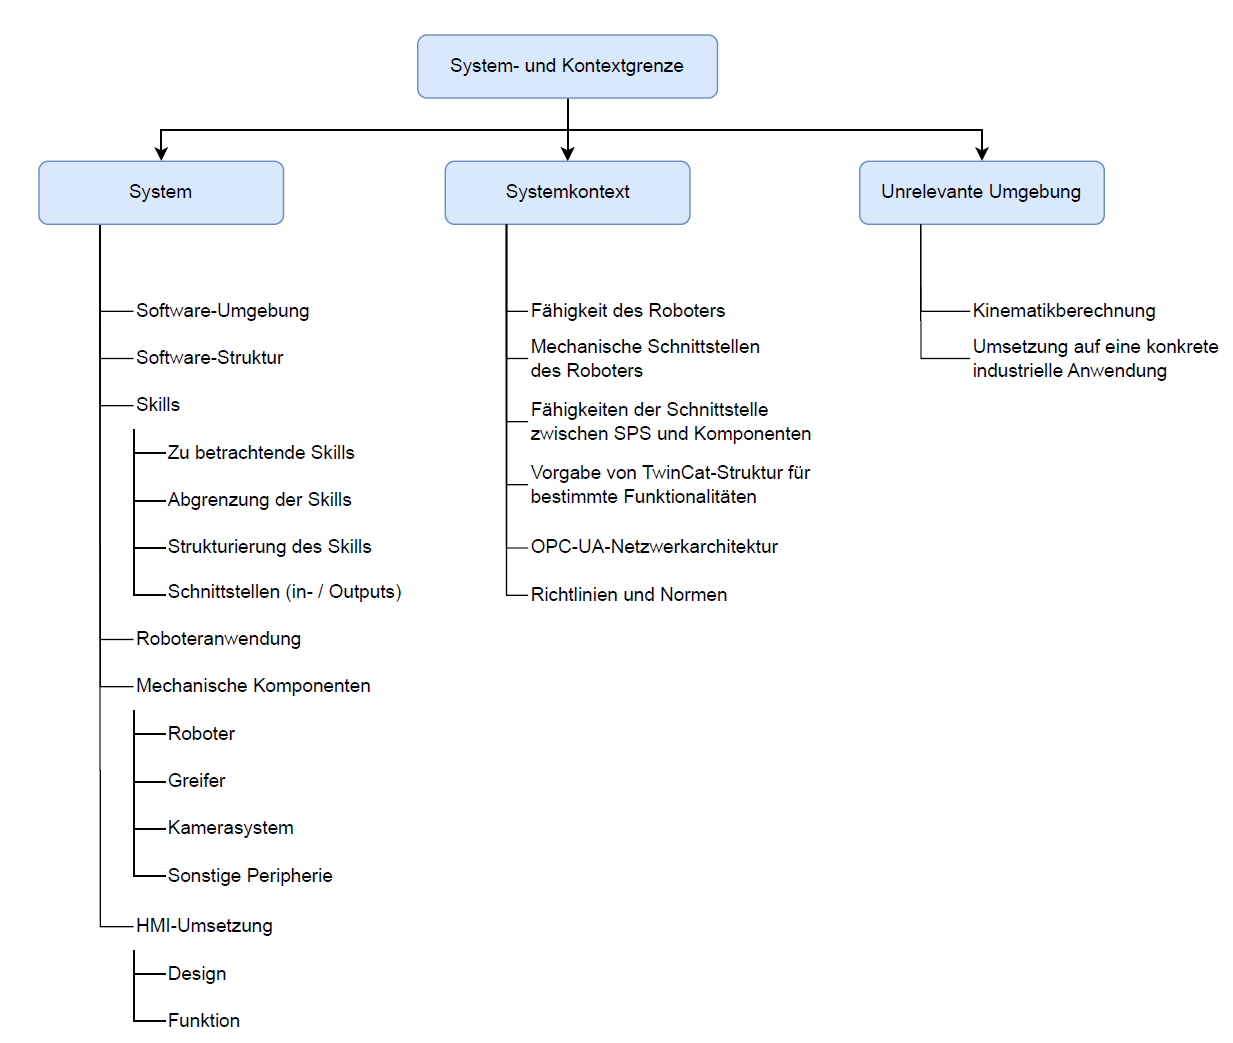
\includegraphics[width=1\textwidth]{02_Einfuehrung_in_Thematik/SystemKontextGrenze}
	\captionsetup{justification=centering}
	\caption{System- und Kontextgrenzen}
	\label{fig:SystemKontextGrenze}
\end{figure}

\newpage
\section{Projektanforderungen} \label{Projektanforderungen}

	Die Thesis basiert auf einem offen definierten Auftrag ohne ein festgelegtes Lastenheft, wodurch die Projektanforderungen entsprechend flexibel gestaltet sind. Um jedoch einen effizienten und zielgerichteten Workflow zu gewährleisten – insbesondere bei einem Projekt dieser Größenordnung – ist es entscheidend, klare Projektziele zu definieren.
	\\
	Für die Definition der Projektanforderungen wird eine bewährte Methode aus dem System- und Anforderungsmanagement genutzt, bei der "Needs", "Goals" und "Objectives" (NGOs) formuliert werden (\ref{tab:Projektanforderungen}). Ein "Need" beschreibt in einer einzigen Aussage, welches Problem das System lösen soll, ohne dabei konkrete Lösungen vorzugeben. Die "Goals" legen die Erwartungen an das System fest, die zur Erfüllung des "Needs" beitragen. Darauf aufbauend definieren die "Objectives" spezifische Anforderungen für jedes "Goal". Ein zentraler Aspekt dieser Anforderungen ist, dass sie messbar, quantifizierbar und überprüfbar sein müssen.
	\\
	\\
	Folgende NGO's wurden für die Thesis definiert: 
	
	\begin{table}[h!]
		\centering
		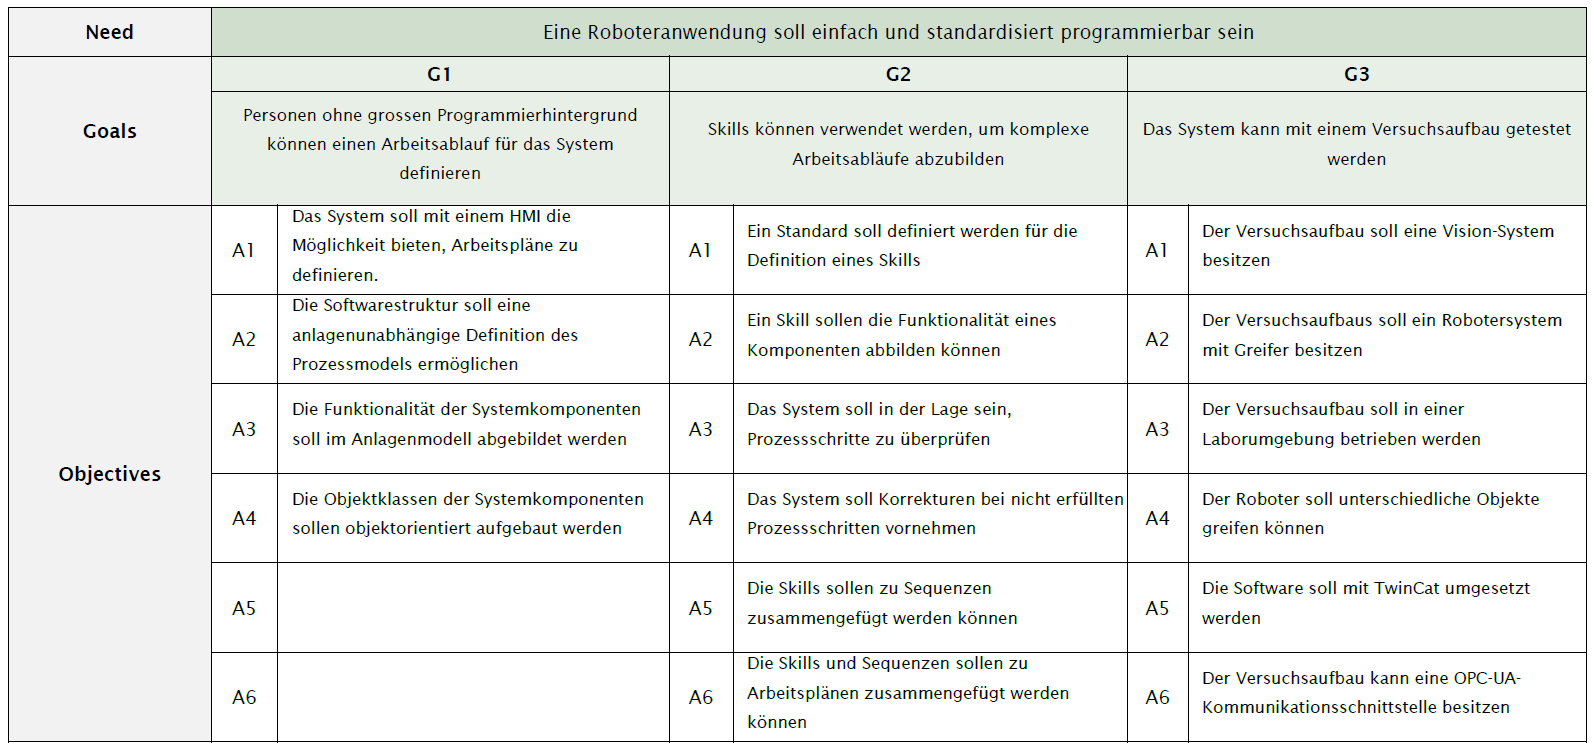
\includegraphics[width=1\textwidth]{02_Einfuehrung_in_Thematik/NGO}
		\caption{Projektanforderungen}
		\label{tab:Projektanforderungen}
	\end{table}

\chapter{Vorgehen} \label{Vorgehen}
Der skill-basierte Ansatz beinhaltet eine Vielzahl unterschiedlicher Aspekte. Für die Thesis ist es daher entscheidend, die Prioritäten klar zu setzen. Zur strukturierten Bearbeitung werden verschiedene Arbeitspakete festgelegt, die die zentralen Anforderungen des Projekts abdecken. Im Anschluss werden die Abhängigkeiten dieser Arbeitspakete bestimmt und in einem Gate-Plan visualisiert. Dieser gliedert die Bearbeitung in Phasen und zeigt die Reihenfolge auf, in der die Arbeitspakete abgearbeitet werden sollen.


\section{Arbeitspakete} \label{Arbeitspakete}

	Grundsätzlich teilt sich das Gesamtsystem in die Hardware und Software ein (Abb. \ref{fig:Arbeitspakete}). Diese lassen sich anschliessend in verschiedene Arbeitspakete aufteilen. 
	\\
	\begin{figure}[h!]
		\centering
		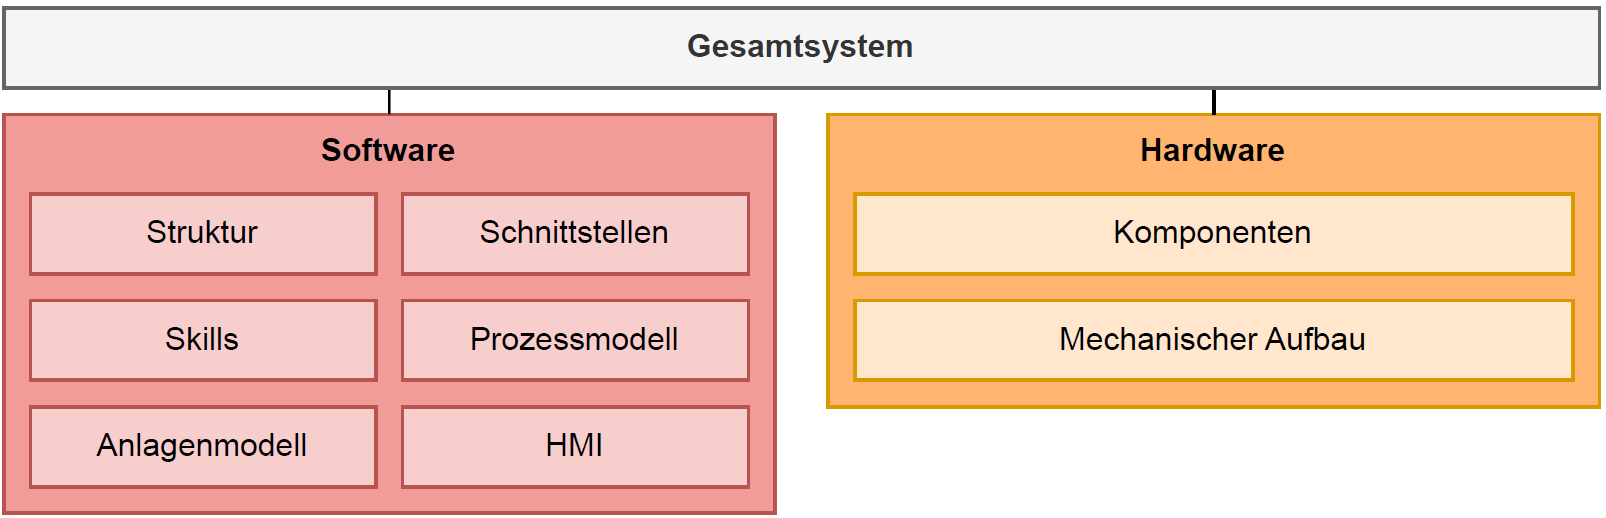
\includegraphics[width=0.7\textwidth]{03_Vorgehen_fuer_die_Thesis/Arbeitspakete}
		\captionsetup{justification=centering}
		\caption{Definierte Arbeitspakete}
		\label{fig:Arbeitspakete}
	\end{figure}
	
	\textbf{Software:} \vspace{2mm} 
	\\
	\begin{tabularx}{\textwidth}{@{}>{}p{7em} X@{}}
		Struktur: & 
		Definieren der Software-Elemente und wie diese miteinander in Beziehung stehen. 
		\\
		
		Schnittstellen: & 
		Definieren der Schnittstellen zwischen Hardware-Komponenten und Software. 
		\\
		
		Skills: & 
		Planung und Entwicklung der Skills (Struktur, Umsetzung).
		\\
		
		Prozessmodell: & 
		Planung und Entwicklung des Prozessmodells (Struktur, Umsetzung).
		\\
		
		Anlagenmodell: & 
		Planung und Entwicklung des Anlagenmodell. (Struktur, Umsetzung).
		\\
		
		\Gls{HMI}: & 
		Planung und Entwicklung des \Gls{HMI}. (Design, Umsetzung, Anwendung).
		\\
	\end{tabularx}
	\vspace{3mm}
	\\
	\textbf{Hardware:} \vspace{2mm} 
	\\
	\begin{tabularx}{\textwidth}{@{}>{}p{7em} X@{}}
		Komponenten: & 
		Definieren einer Anwendung und die dazu benötigten Komponenten.
		\\
		
		Mech. Aufbau: & 
		Konstruktion und Montage des mechanischen Aufbaus.
		\\
	\end{tabularx}
	
	\newpage


\section{Gate-Plan} \label{Gate-Plan}

	Der Gate-Plan besteht aus 4 Phasen (\ref{fig:Gateplan}). Jede Phase wird durch ein Gate begonnen und abgeschlossen. Innerhalb der Phasen werden die verschiedenen Arbeitspakete erarbeitet. 

	\begin{figure}[h!]
		\centering
		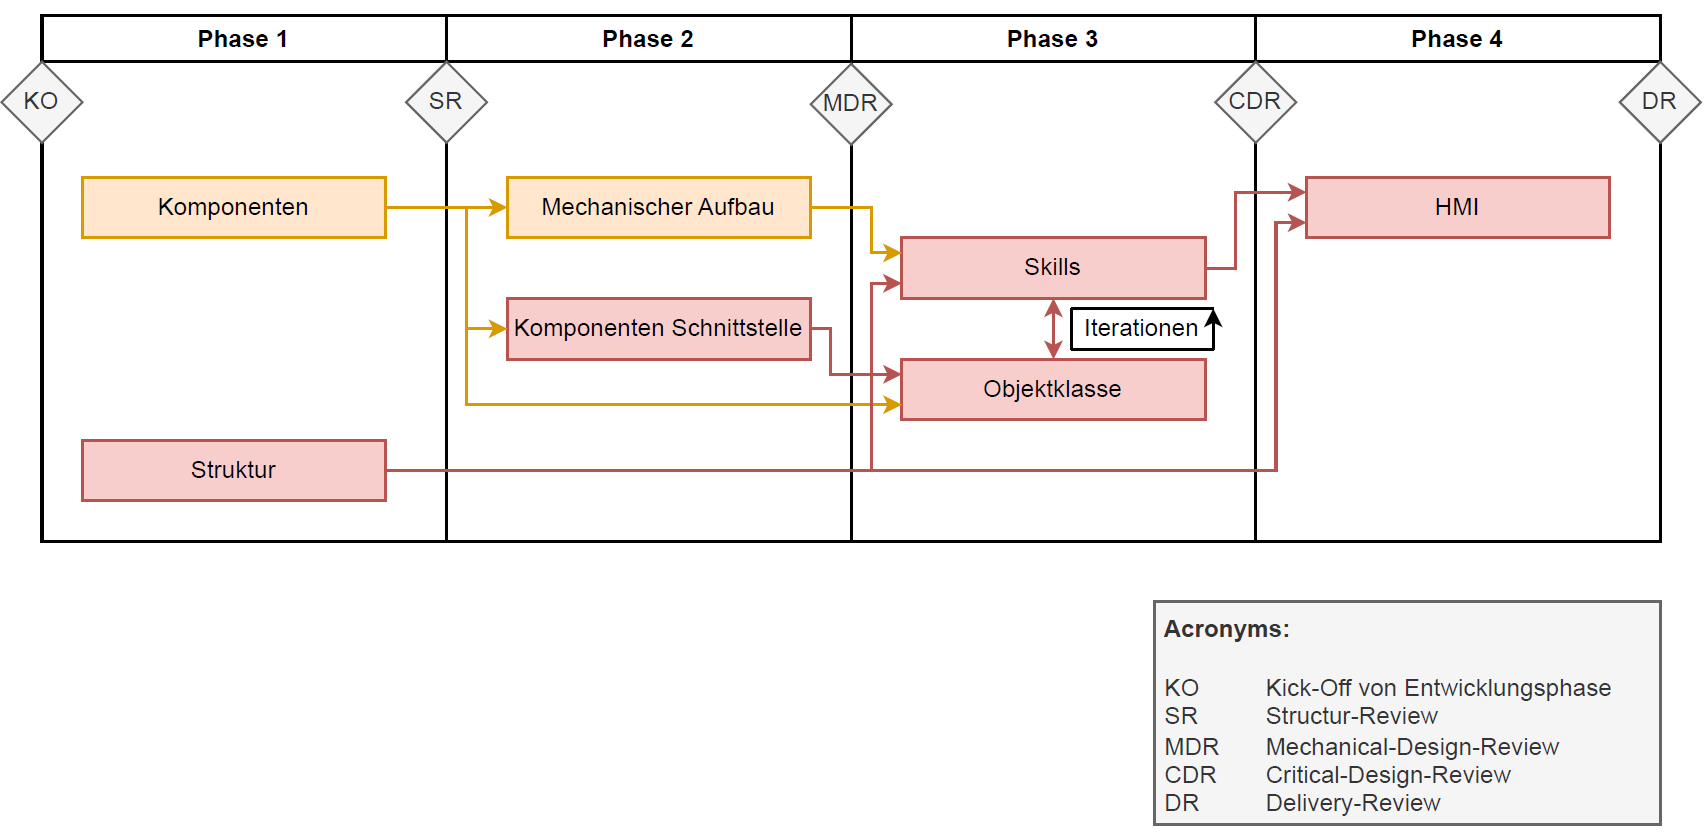
\includegraphics[width=1\textwidth]{03_Vorgehen_fuer_die_Thesis/Gateplan}
		\captionsetup{justification=centering}
		\caption{Definierter Gate-Plan}
		\label{fig:Gateplan}
	\end{figure}
	
	\textbf{Phase 1:} \vspace{2mm} 
	\\
		\begin{tabularx}{\textwidth}{@{}>{}p{7em} X@{}}
			Beschreibung: & 
			Phase 1 beschäftigt sich mit den Grundlagen der Hard- und Software. Die relevanten Komponenten müssen definiert und die notwendigen Fragen bezüglich der Software-Struktur geklärt werden.
			\\
			
			Output: & 
			\begin{itemize}
				\item Alle Komponenten für den Versuchsaufbau sind bekannt
				\item Die allgemeine Software-Struktur wurde definiert
			\end{itemize}
		\end{tabularx}
	
	\textbf{Phase 2:} \vspace{2mm} 
	\\
		\begin{tabularx}{\textwidth}{@{}>{}p{7em} X@{}}
			Beschreibung: & 
			Innerhalb von Phase 2 wird der Hardware-Teil abgeschlossen. Dafür wird der Versuchsaufbau konstruiert und gebaut. Zusätzlich werden die Software-Schnittstellen der Komponenten analysiert und definiert. 
			\\
			
			Output: & 
			\begin{itemize}
				\item Gebauter Versuchsbau für das Testen der Software
				\item Es ist bekannt, wie die Komponenten in die Software implementiert werden (in Theorie)
			\end{itemize}
		\end{tabularx}
	
	\textbf{Phase 3:} \vspace{2mm} 
	\\
		\begin{tabularx}{\textwidth}{@{}>{}p{7em} X@{}}
			Beschreibung: & 
			Phase 3 stellt die konkrete Umsetzung des skill-basierten Ansatzes in der Software dar. Hierbei wird iterativ die Software entwickelt. Die umfasst die Umsetzung der Struktur, wie auch die Entwicklung der Skills, der Objektklassen und des kompletten Prozessmodells.  
			\\
	
			Output: & 
			\begin{itemize}
				\item Funktionaler Prototyp, welcher an der Versuchsanlage getestet werden kann
			\end{itemize}
		\end{tabularx}
	
	\textbf{Phase 4:} \vspace{2mm} 
	\\
		\begin{tabularx}{\textwidth}{@{}>{}p{7em} X@{}}
			Beschreibung: & 
			Die letzte Phase beschäftigt sich mit der Entwicklung eines HMI.  
			\\
			
			Output: & 
			\begin{itemize}
				\item Über HMI bedienbarer Prototyp, welcher an der Versuchsanlage getestet werden kann
			\end{itemize}
		\end{tabularx}
	
	

\chapter{Anwendung und Aufbau} \label{Anwendung und Aufbau}
\section{Definition der Anwendung} \label{Anwendungsdefinition}
	Als Anwendung für den Versuchsaufbau wurde die Verbindung zweier Platten über einen Befestigungswinkel definiert. Die Platten bestehen aus Kunststoff und sind mit drei Befestigungslöcher, wie auch Fingerzinken versehen. Der Prozess wird durch 3 Teilprozesse gebildet. 
	\vspace{3mm}
	
	\textbf{Teilprozess 1:} Positionieren der Platten
	\vspace{2mm} 
	\\
	 Der Teilprozess fügt die beiden Platten im 90°-Winkel zusammen (\ref{fig:Teilprozess 1}). Die Seiten der Platten sind mit Fingerzinken versehen, die ineinandergreifen. Der Roboter entnimmt zunächst die erste Platte aus dem Lager und positioniert sie auf einer Halterung. Anschliessend holt der Roboter die zweite Platte und stosst diese entsprechend der Fingerzinken in die erste Platte.
	 \vspace{3mm} 
	 
	 \textbf{Teilprozess 2:} Montieren von Befestigungswinkel 
	 \vspace{2mm}
	 \\
	 Der Roboter holt den Befestigungswinkel aus dem Lager und platziert diesen entsprechend der Löcher in den Platten (\ref{fig:Teilprozess 2}). Die korrekte Position wird über ein Vision-System definiert. Das Befestigungsblech kann auch in die Halterung eingelegt werden.
	 \vspace{3mm}
	 
	 \textbf{Teilprozess 3:} Verbinden von Platten mit Befestigungswinkel 
	 \vspace{2mm} 
	 \\
	 Im letzten Schritt werden die Befestigungswinkel via Stifte mit den Platten verbunden (\ref{fig:Teilprozess 3}). Die Passung der Löcher ist dabei so ausgelegt, dass der Stift knapp mit Spiel montiert werden kann. Die Stifte müssen somit so mit der Platte verbunden werden, dass sich diese nicht verkanten. 
	 \vspace{3mm}
	 
	 \begin{figure}[h!]
	 	\centering
	 	\begin{subfigure}[b]{0.28\textwidth}
	 		\centering
	 		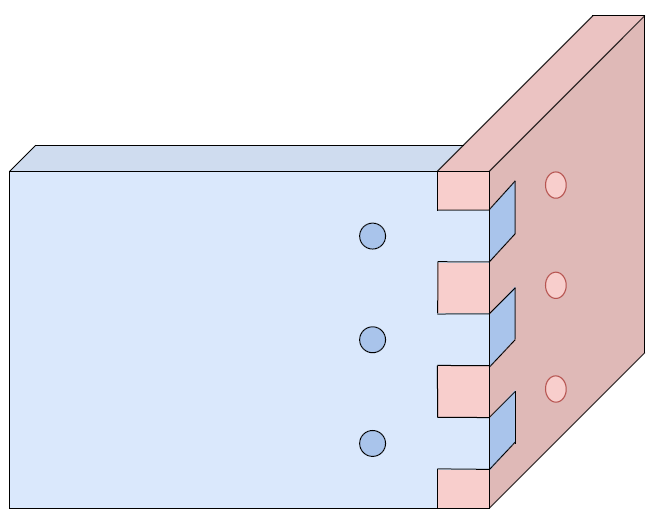
\includegraphics[width=\textwidth]{04_Anwendung_und_Aufbau/Teilprozess_1}
	 		\caption{Teilprozess 1}
	 		\label{fig:Teilprozess 1}
	 	\end{subfigure}
	 	\hfill
	 	\begin{subfigure}[b]{0.28\textwidth}
	 		\centering
	 		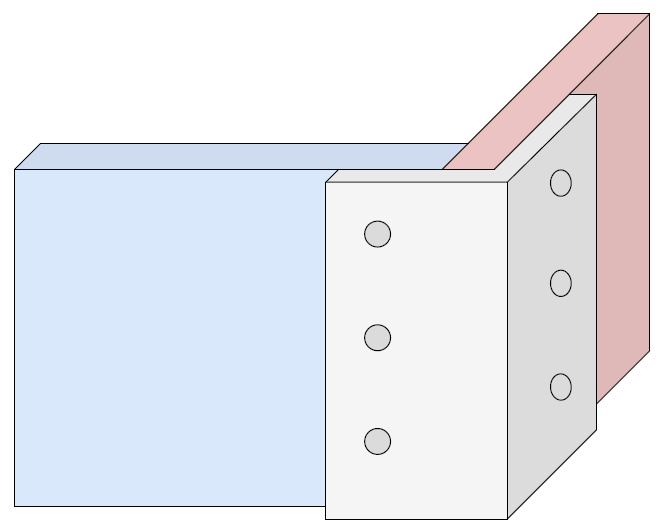
\includegraphics[width=\textwidth]{04_Anwendung_und_Aufbau/Teilprozess_2}
	 		\caption{Teilprozess 2}
	 		\label{fig:Teilprozess 2}
	 	\end{subfigure}
	 	\hfill
	 	\begin{subfigure}[b]{0.32\textwidth}
	 		\centering
	 		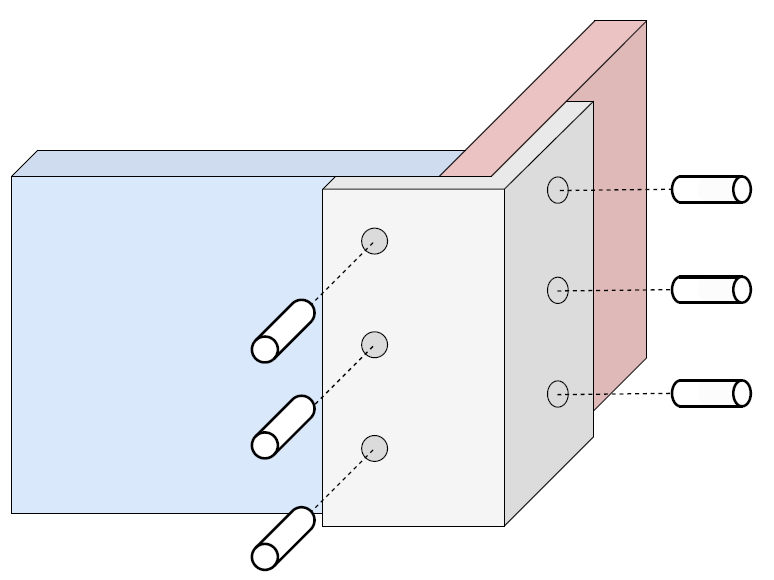
\includegraphics[width=\textwidth]{04_Anwendung_und_Aufbau/Teilprozess_3}
	 		\caption{Teilprozess 3}
	 		\label{fig:Teilprozess 3}
	 	\end{subfigure}
	 	\caption{Anwendungsteilprozesse}
	 	\label{fig:Teilprozesse}
	 \end{figure}
	 
	
	 \newpage
	 
\section{Definition der Anlagenkomponenten} \label{Anlagenkomponenten}
	Die allgemeine Kommunikationstopologie (\ref{fig:Kommunikationstopologie}) der funktionsrelevanten Komponenten sieht wie folgt aus: 
	
	\begin{figure}[h!]
		\centering
		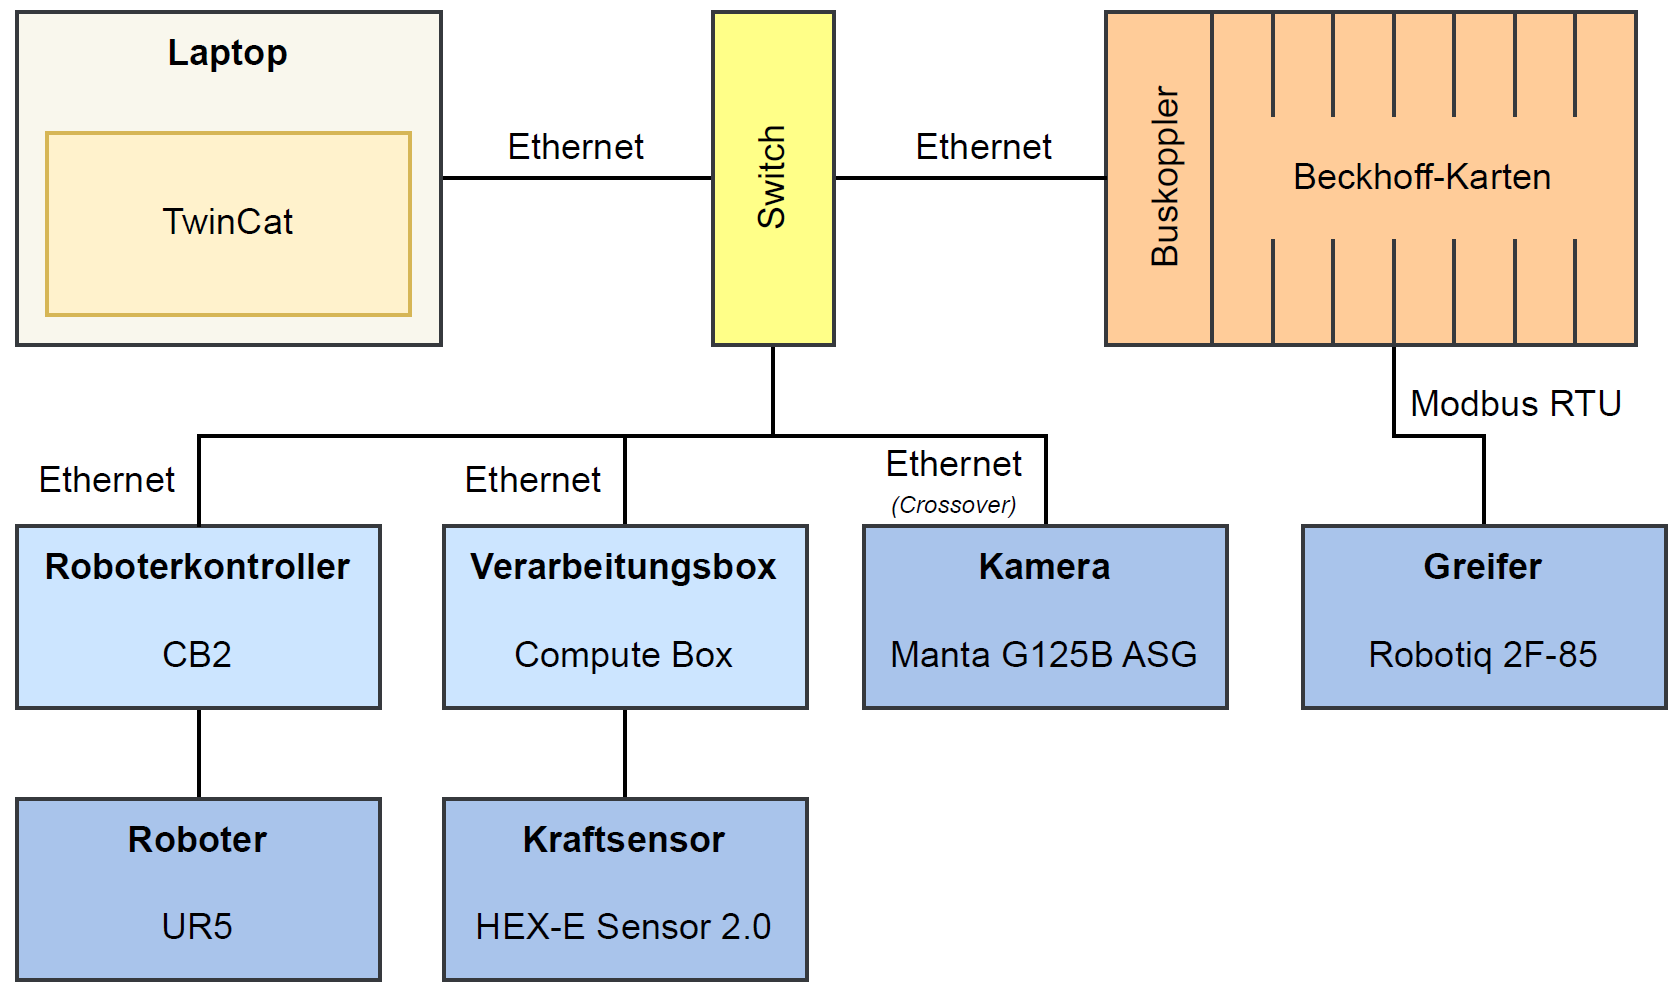
\includegraphics[width=0.8\textwidth]{04_Anwendung_und_Aufbau/Kommunikationstopologie}
		\captionsetup{justification=centering}
		\caption{Kommunikationstopologie}
		\label{fig:Kommunikationstopologie}
	\end{figure}
	
	Für die Umsetzung des Versuchsaufbaus wird ein Laptop mit TwinCAT als SPS eingesetzt. Der Grund dafür ist die Leistungsfähigkeit. Da alle Funktionalitäten innerhalb der SPS stattfinden sollen, muss diese auch die entsprechende Power mitbringen. 
	\\
	Die Switch verbindet den Laptop mit dem Bus-Koppler und den entsprechenden Komponenten der Prozesszelle. Teil des Netzwerkes ist der Roboterkontroller, die Signalverarbeitungsbox des Kraftsensors und die Kamera. 
	
	\textbf{Roboter und Roboterkontroller:}
	\vspace{2mm} 
	\\
	Der UR5-Roboter von Universal Robots wurde als Robotersystem ausgewählt. Dieser kollaborative Roboter zeichnet sich durch eine benutzerfreundliche Kommunikationsschnittstelle aus und kann schnell und unkompliziert in Betrieb genommen werden. An der BFH besteht umfassende Erfahrung mit dem UR5, und es stehen verschiedene Peripherie-Tools zur Verfügung.
	\\
	Mit einer Traglast von 5 kg und einer Reichweite von 850 mm ist der Roboter für vielfältige Anwendungen geeignet. Als Kommunikationsschnittstelle zwischen TwinCAT und Kontroller wird eine TCP/IP-Schnittstelle verwendet. Dafür muss TwinCAT mit dem TF6310-Paket (TwinCAT 3 TCP/IP) oder TF6311-Paket (TwinCAT 3 TCP/UDP Realtime) versehen werden, wobei TF6310 auch eine UDP-Kommunikation aufbauen kann. Bei TF6311 wird jedoch direkt über die Netzwerkkarte mit dem Server oder Client kommuniziert, was eine spezielle Hardwareschnittstelle voraussetzt. Diese Schnittstellen ermöglicht das Programmieren des Roboters über URScript. Der Kontroller verfügt aber auch über digitale und analoge Ein- und Ausgänge. 
	
	\textbf{Kamera:}
	\vspace{2mm} 
	\\
	Als Kamera kommt die „Manta G125B ASG“ zum Einsatz, die mit der weit verbreiteten GigE-Vision-Schnittstelle ausgestattet ist. Dadurch lässt sie sich direkt aus TwinCAT auslesen und konfigurieren. Um die Kamera in Betrieb zu nehmen, müssen die TF7XXX-Pakete (TwinCAT 3 Vision) installiert sein. Der Anschluss der Kamera erfolgt über eine Ethernet-Schnittstelle mithilfe eines Crossover-Kabels.
	
	\textbf{Kraftmessungssensor:}
	\vspace{2mm} 
	\vspace{-3mm} 
	\vspace{-\baselineskip}
	\vspace{-\baselineskip}
	\\
	\begin{wrapfigure}{r}{0.35\textwidth}
		\centering
		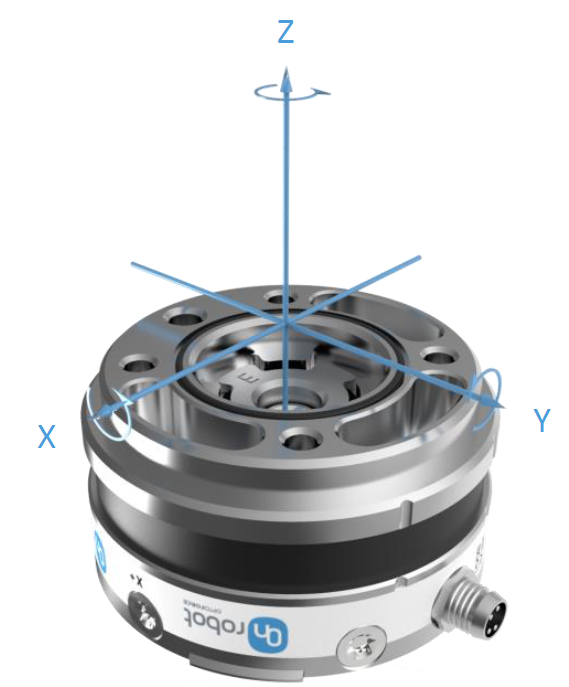
\includegraphics[width=0.35\textwidth]{04_Anwendung_und_Aufbau/Kraftsensor}
		\captionsetup{justification=centering}
		\caption{Kraftsensor}
		\label{fig:Kraft_sensor}
	\end{wrapfigure} \par
	Im Gegensatz zum UR5e verfügt der UR5 über keine integrierten Kraft-/Drehmomentsensoren in den Gelenken, was eine präzise Kraftregelung erschwert. Um dies zu kompensieren, kann der UR5 mit einem externen Kraftmesssensor ausgestattet werden. Hierfür eignet sich der „HEX-E Sensor 2.0“ von OnRobot (\ref{fig:Kraft_sensor}), der an der mechanischen Schnittstelle des UR5 montiert werden kann. 
	\\
	Der Sensor misst Kräfte und Drehmomente in und um drei Achsen. Die erfassten Daten werden an eine Signalverarbeitungsbox weitergeleitet, die das Rohsignal verarbeitet und über eine Ethernet-Schnittstelle zur Verfügung stellt. Die Kommunikation kann über eine UDP- oder TCP-Schnittstelle erfolgen. Für die Integration in TwinCAT kann das TF6310-Paket (TwinCAT 3 TCP/IP) verwendet.
	
	\textbf{Greifer:}
	\vspace{2mm} 
	\\
	Für das System wird der 2F-85-Greifer von Robotiq verwendet (\ref{fig:Greifer}), der speziell für die Integration mit UR-Robotern entwickelt wurde. Die Montage erfolgt einfach mittels einer Adapterplatte, und der Greifer wird direkt über den Anschluss am UR5-Roboter verbunden. Der eingesetzte CB2-Kontroller ist gerade noch in der Lage den Greifer betreiben zu können. 
	
	\begin{figure}[h!]
		\centering
		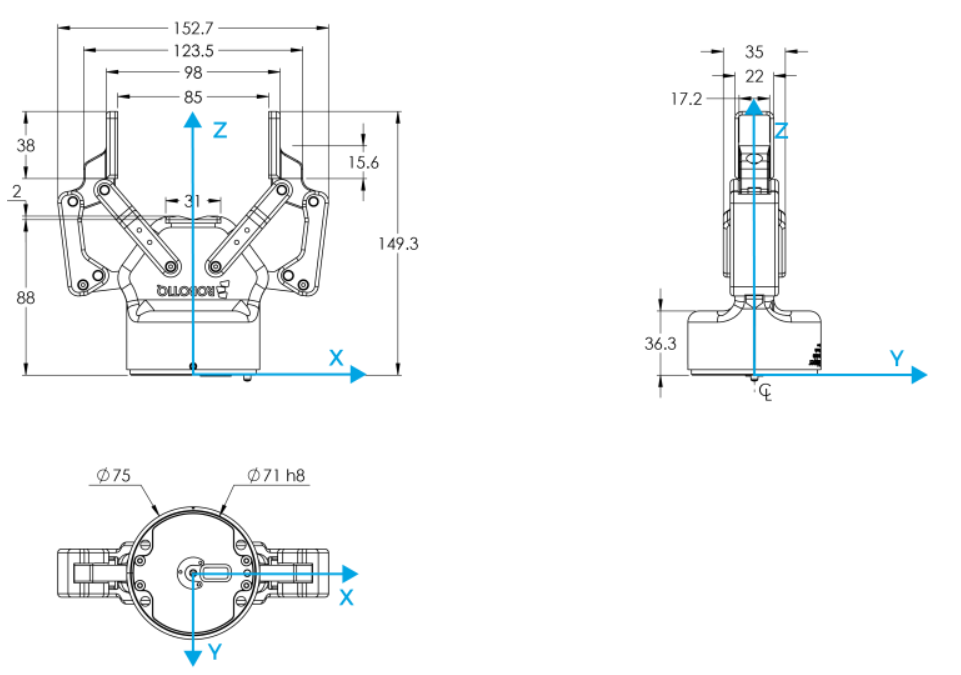
\includegraphics[width=1\textwidth]{04_Anwendung_und_Aufbau/Greifer}
		\captionsetup{justification=centering}
		\caption{Kommunikationstopologie}
		\label{fig:Greifer}
	\end{figure}
	
	Der 2F-85-Greifer bietet eine maximale Greifweite von 85 mm und wird elektrisch betrieben. Dank integrierter Sensoren lässt sich die Greifkraft präzise überwachen und anpassen. Auch die Fingerposition wird überwacht, was dem Greifer eine hohe Flexibilität in verschiedenen Anwendungen ermöglicht.
\section{Mechanischer Aufbau} \label{Mechanischer_Aufbau}
	Die mechanische Konstruktion wurde so einfach wie möglich gestaltet, um in erster Linie das schnelle Testen der Software zu ermöglichen. Der Aufbau besteht aus zwei Kunststoffplatten, einem Verbindungsblech und vier Stiften.
	\\
	Der Montageprozess erfolgt in drei Schritten: Zunächst werden die beiden Platten miteinander verbunden (\ref{fig:Montageschritt 1}). Dafür sind sie mit sogenannten "Fingerzinkungen" ausgestattet, durch die sie ineinandergesteckt werden. Anders als im ursprünglichen Konzept vorgesehen, bei dem eine Eckverbindung angedacht war (siehe Verweis), liegen die Platten in einer Ebene. Erste Simulationen mit der Software „RoboDK“ ergaben, dass eine Umsetzung mit Eckverbindung die Erreichbarkeit der verschiedenen Positionen für den Roboter deutlich erschwert hätte. Durch den montierten Kraftsensor und Greifer wird der TCP versetzt, wodurch der Arbeitsbereich des Roboters zusätzlich eingeschränkt wird. Die flache Anordnung der Platten erleichtert die Zugänglichkeit erheblich, während der grundlegende Prozess unverändert bleibt.
	\\
	Im zweiten Schritt wird das Verbindungsblech auf die zusammengefügten Platten aufgelegt (\ref{fig:Montageschritt 2}). Es muss dabei exakt auf die Lochpositionen der Platten ausgerichtet werden. Im dritten Schritt werden die Platten und das Blech mithilfe von Stiften fixiert (\ref{fig:Montageschritt 3}). Die Stifte werden in die vorgesehenen Löcher gedrückt, wobei eine enge, aber noch als Spielpassung definierte Toleranz vorliegt. Der Roboter muss dabei äusserst präzise arbeiten und in der Lage sein, eine Verkantung zu erkennen. Auf Verfahren wie Schrauben oder Nieten wurde bewusst verzichtet, um den Einsatz eines spezifischen Werkzeugs für den Roboter zu vermeiden.
	
	 \begin{figure}[h!]
		\centering
		\begin{subfigure}[b]{0.3\textwidth}
			\centering
			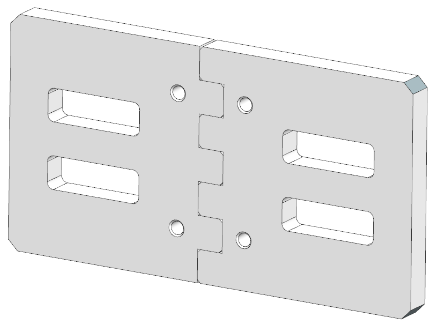
\includegraphics[width=\textwidth]{04_Anwendung_und_Aufbau/Montageschritt_1}
			\caption{Montageschritt 1}
			\label{fig:Montageschritt 1}
		\end{subfigure}
		\hfill
		\begin{subfigure}[b]{0.3\textwidth}
			\centering
			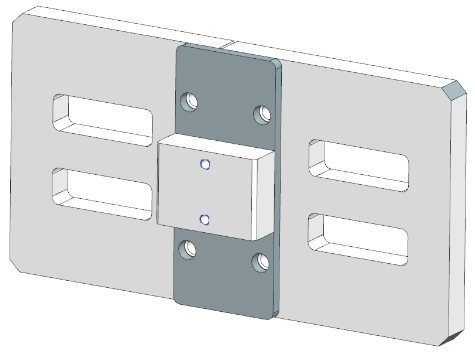
\includegraphics[width=\textwidth]{04_Anwendung_und_Aufbau/Montageschritt_2}
			\caption{Montageschritt 2}
			\label{fig:Montageschritt 2}
		\end{subfigure}
		\hfill
		\begin{subfigure}[b]{0.3\textwidth}
			\centering
			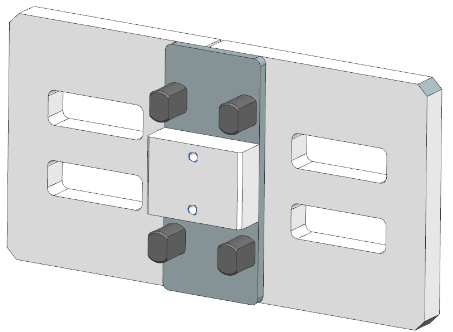
\includegraphics[width=\textwidth]{04_Anwendung_und_Aufbau/Montageschritt_3}
			\caption{Montageschritt 3}
			\label{fig:Montageschritt 3}
		\end{subfigure}
		\caption{Anwendungsteilprozesse}
		\label{fig:Montageschritte}
	\end{figure}
	
	\begin{bfhNoteBox}
		Alle Detailzeichnungen in Fertigungsdaten werden im Anhang beigelt. 
	\end{bfhNoteBox}	
	
	\vspace{5mm} 
	\begin{wrapfigure}{r}{0.6\textwidth}
		\centering
		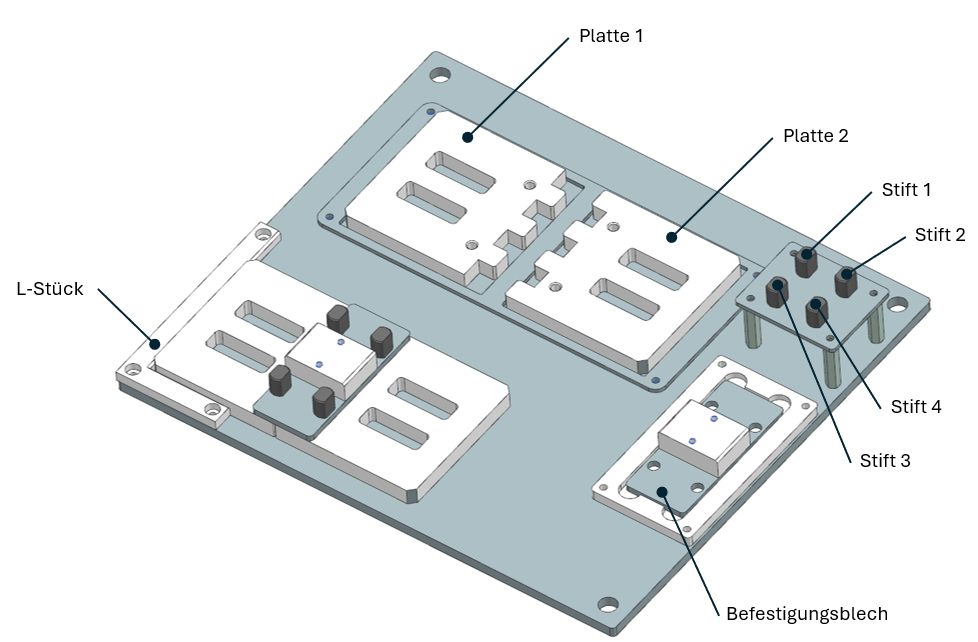
\includegraphics[width=0.6\textwidth]{04_Anwendung_und_Aufbau/Montagevorrichtung}
		\captionsetup{justification=centering}
		\caption{Montagevorrichtung}
		\label{fig:Montagevorrichtung}
	\end{wrapfigure} \par
	Die Montage wird auf einer Platte durchgeführt, welche gleichzeitig auch als Halterung für Komponenten dient (\ref{fig:Montagevorrichtung}). Im unteren linken Bereich werden die Komponenten montiert. Dafür wird das Kunststoff-L-Stück als Anschlag verwendet. 
	
	

\chapter{Struktur der Software} \label{Struktur der Software}
Die Struktur der Software muss auf einen skill-basierten Ansatz ausgelegt werden. Dafür müssen die Anforderungen an eine solche Struktur klar definiert und die Möglichkeiten, die TwinCAT bietet, analysiert werden. In einem ersten Schritt wird die allgemeine Grobstruktur des Systems dargestellt (Abb. \ref{fig:Strukturübersicht}). Dieses kann wie folgt definiert werden: 

\begin{figure}[h!]
	\centering
	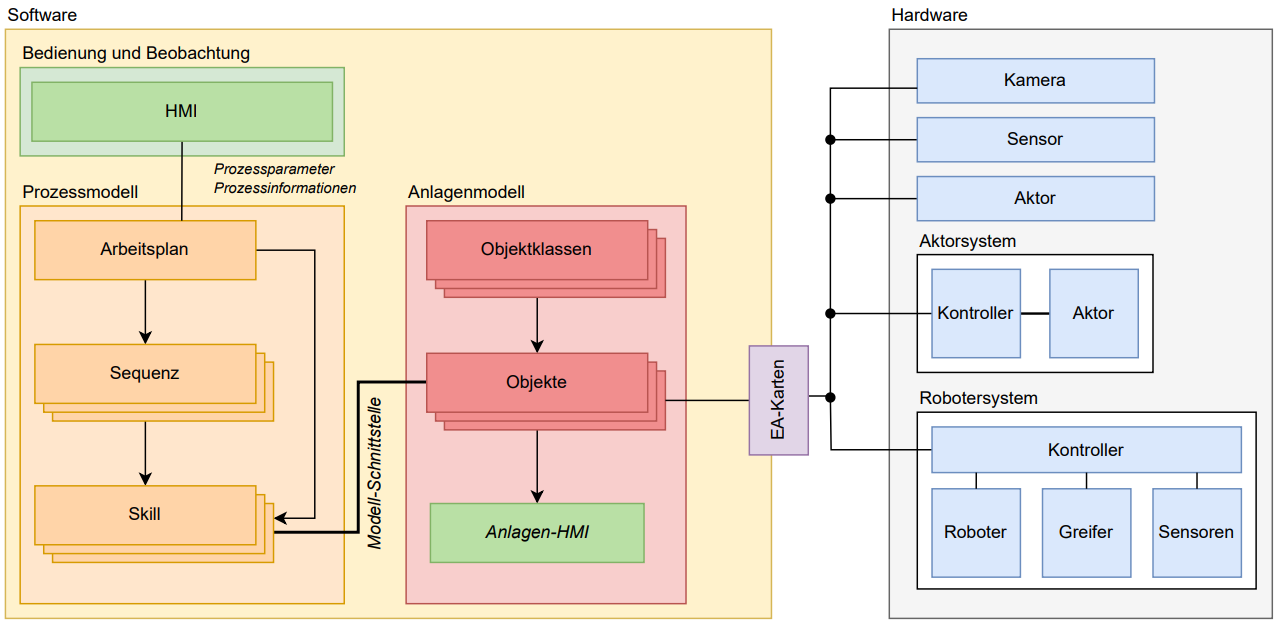
\includegraphics[width=1\textwidth]{05_Softwarestruktur/Overview}
	\captionsetup{justification=centering}
	\caption{Strukturübersicht}
	\label{fig:Strukturübersicht}
\end{figure}

Wie durch die ANSI/ISA-88-Norm vorgegeben (beschrieben in Kapitel \ref{Fragen bezüglich Referenzprojekt}), besteht die Software aus einem Prozess- und einem Anlagenmodell. Das Prozessmodell steuert den Ablauf, während das Anlagenmodell die Schnittstelle zu den einzelnen Anlagenkomponenten darstellt. Innerhalb des Prozessmodells werden die Skills definiert, die entweder von Sequenzen oder direkt aus dem Arbeitsplan zur Ablaufsteuerung genutzt werden können. Der Arbeitsplan beschreibt den gesamten Prozess.
\\
Das Anlagenmodell implementiert die Objektklassen der verschiedenen Systemelemente und bildet deren Funktionalitäten ab. Die Struktur des Anlagenmodells ist klar und übersichtlich: Die Objektklassen werden instanziiert und diese Objekte mit den entsprechenden Ein- und Ausgängen verknüpft, welche die Schnittstelle zum realen System darstellen. Der Grundgedanke dabei ist, dass alle Funktionalitäten zentral in der \Gls{SPS} gebündelt werden, um möglichst wenig Funktionalität auf den einzelnen Komponenten selbst zu belassen. Ziel ist es, dass sämtliche Elemente, von Robotern bis zu Kameras, über die \Gls{SPS} gesteuert werden können. Voraussetzung dafür ist, dass alle Komponenten über eine funktionale Schnittstelle zur \Gls{SPS} verfügen. Alle Komponenten werden im Anlagen-HMI visualisiert und können dort manuell gesteuert werden. Dies ermöglicht es beispielsweise, Roboterpositionen zu speichern, die später von einem Skill für Bewegungsabläufe genutzt werden können. 
\\
Abschliessend gibt es eine Bedienungs- und Beobachtungsebene, die als Benutzerschnittstelle dient, um Prozessparameter einzugeben und Informationen über den Prozess anzuzeigen. Diese Systemstruktur ermöglicht auch den modularen Aufbau von Systemen (Abb. \ref{fig:Gesamtsystemstruktur}). Das folgende Schema zeigt, wie ein solches System aussehen könnte:

\begin{figure}[h!]
	\centering
	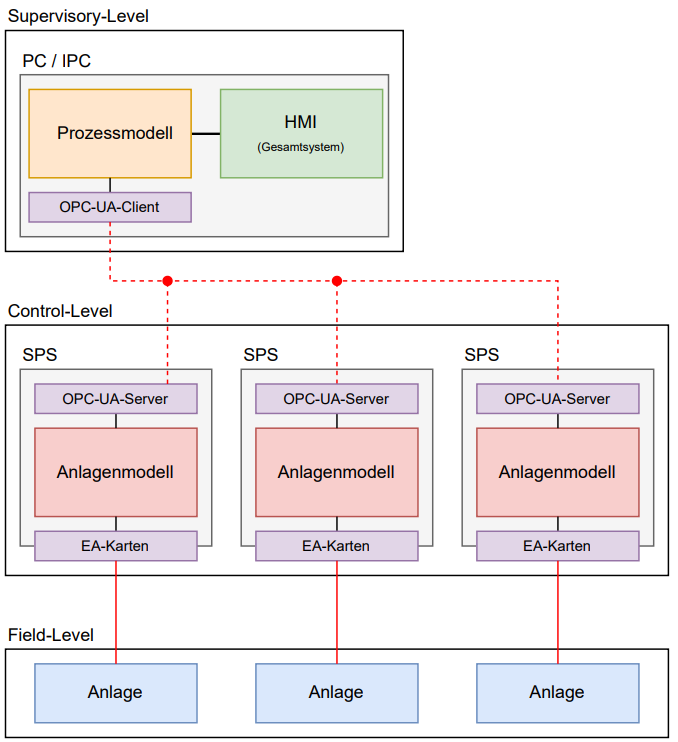
\includegraphics[width=0.5\textwidth]{05_Softwarestruktur/Gesamtsystemstruktur}
	\captionsetup{justification=centering}
	\caption{Gesamtsystemstruktur}
	\label{fig:Gesamtsystemstruktur}
\end{figure}

Das Schema orientiert sich an der Automatisierungspyramide \cite{Automatisierungspyramide} und zeigt die ersten drei Ebenen (Supervisory-, Control- und Field-Level). Dabei handelt es sich um ein System, welches aus verschiedenen Teilanlagen besten, mit eigener \Gls{SPS} und Anlagenmodell. Auf dem Supervisory-Level befindet sich das Prozessmodell. Hier wird über die HMI ein Arbeitsplan ausgewählt / zusammengestellt und gestartet. Eine OPC-UA-Schnittstelle übermittelt die prozessrelevanten Daten an die entsprechende \Gls{SPS} im Control-Level. Die \Gls{SPS} steuert die Anlage im Field-Level basierend auf dem Anlagenmodell. Die verschiedenen Anlagen können flexibel für unterschiedliche Aufgaben genutzt werden oder, falls sie identische Fähigkeiten besitzen, nach Auslastung zugewiesen werden. Dadurch ist das System äusserst flexibel und kann ohne grossen Aufwand erweitert werden.

\section{Schnittstellen innerhalb der Software} \label{Softwareschnittstellen}

	Die Software besteht aus den drei Hauptelementen: Bedienung und Beobachtung (HMI), Prozessmodell und Anlagenmodell (Abb. \ref{fig:Strukturübersicht}). Um die Schnittstellen zwischen diesen Elementen zu definieren, müssen die Kompetenzen klar definiert werden. Wer ist für was verantwortlich und welche Informationen werden dafür benötigt. 
	
	\textbf{Bedienung und Beobachtung:}
	\vspace{2mm} 
	\\
	Über das HMI wird der Arbeitsplan erstellt und mit den erforderlichen Ablaufparameter versehen. Das System sowie der erstellte Arbeitsplan können über das HMI gestartet, gestoppt und gesteuert werden.
	
	\textbf{Prozessmodell:}
	\vspace{2mm} 
	\\
	Das Prozessmodell koordiniert die Ausführung des Arbeitsplans. Zusammen mit den Ablaufparameter werden die Prozessparameter festgelegt und weitergegeben. Der Arbeitsplan wird in einzelne Skills unterteilt, die wiederum die grundlegenden Funktionen der Anlagenkomponenten ausführen. Die effiziente und standardisierte Definition eines Skills, vereinfacht die Anwendung dieser in den Sequenzen und Arbeitsplänen.
	
	\newpage
	
	\textbf{Anlagenmodell:}
	\vspace{2mm} 
	\\
	Das Anlagenmodell bildet die Funktionalität der Systemkomponenten ab. Es stellt die Funktionen durch Methoden dar, während Zustände und Prozessinformationen über Eigenschaften wiedergegeben werden. Das Anlagenmodell verarbeitet die erhaltenen Prozessparameter und übersetzt diese in Anlagenparameter, mit denen die Komponenten der Anlage betrieben werden. Die vom Anlagenmodell zurückgemeldeten Daten (wie Zustände und Messwerte) werden als Zustandsparameter bezeichnet. 
	\\
	\vspace{-13mm}
	\begin{wrapfigure}{r}{0.35\textwidth}
		\centering
		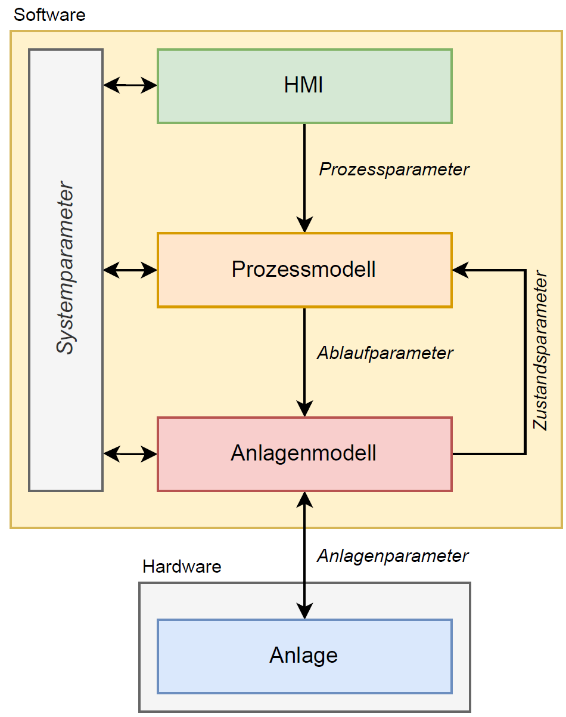
\includegraphics[width=0.3\textwidth]{05_Softwarestruktur/Systemstruktur}
		\captionsetup{justification=centering}
		\caption{Systemstruktur}
		\label{fig:Systemstruktur}
	\end{wrapfigure} \par
	Die drei Hauptelemente müssen voneinander abgegrenzt werden (Abb. \ref{fig:Systemstruktur}). Der modellbasierte Ansatz der Softwarestruktur bietet dabei mehrere Vorteile (siehe EVA-Referenz). Dank klarer Struktur und Übersichtlichkeit lassen sich die Prozesse und Abläufe leicht nachvollziehen. Dies erleichtert die Kommunikation, da durch die einheitliche Verwendung von Begriffen alle dieselbe «Sprache» sprechen. Darüber hinaus können Risiken früher und einfacher erkannt werden.
	\\
	Die Abgrenzung der Hauptelemente geschieht über die Schnittstellen zwischen diesen. Die Schnittstellen werden durch die verschiedenen Parameter definiert. Der Begriff Parameter ist dabei ein Sammelbegriff für alle definierten Variablen, welche zwischen den Elementen ausgetauscht werden.
	
	\textbf{Prozessparameter:}
	\vspace{2mm} 
	\\
	Die Prozessparameter beschreiben den Prozess auf eine möglichst einfache Weise. Es werden nur Informationen weitergegeben, welche nötig sind um den Prozess eindeutig zu definieren. Die Prozessparameter hängen dabei von den Skills und deren Fähigkeiten ab. Die Parameter werden während der Erarbeitung des Prozessmodells definiert.
	
	\textbf{Ablaufparameter:}
	\vspace{2mm} 
	\\
	Ablaufparameter werden durch die Skills definiert und legen relevante Parameter für den Ablauf fest. Die Informationen sind jedoch nicht konkret auf die Komponenten im System ausgelegt. Die Ablaufparameter sind noch anlagenunabhängig und hängen z.B. nicht vom Typ des Roboters ab, welcher im System eingesetzt wird. Die genauen Parameter werden während der Erarbeitung des Prozessmodells definiert.
	
	\textbf{Anlagenparameter:}
	\vspace{2mm} 
	\\
	Die Parameter, welche von den instanziierten Objekten im Anlagemodell vorbereitet werden, dienen als Schnittstelle zur realen Anlage und sind anlagenspezifisch. Die Art dieser Parameter hängt von den eingesetzten Komponenten im System ab. Die genauen Parameter werden während der Erarbeitung des Anlagenmodells definiert.
	
	\textbf{Zustandsparameter:}
	\vspace{2mm} 
	\\
	Die durch die instanziierten Objekte ausgewerteten und verarbeiteten Anlagenparameter werden als Zustandsparameter an das Prozessmodell zurückgegeben. Auf diese Parameter reagiert der Skill wie auch das System. Die genauen Parameter werden während der Erarbeitung des Anlagenmodells definiert.
	
	\textbf{Systemparameter:}
	\vspace{2mm} 
	\\
	Systemparameter sind systemübergreifende Parameter, welche zur Bedienung des gesamten Systems verwendet werden oder dessen Zustand darstellen. 
\section{Interaktion innerhalb der Software} \label{Softwareinteraktion}

	Um die Schnittstellen innerhalb der Software besser zu verstehen, muss die Interaktion zwischen Systemparameter, Prozessmodell (Skills) und Anlagemodell (Objekten) abgegrenzt sein, da diese die wichtigsten Schnittstellen im System darstellen (Abb. \ref{fig:Schnittstellenübersicht}). Die Interaktion findet dabei mit 3 Schnittstellen statt. 
	
	\textbf{Objektschnittstelle:}
	\vspace{2mm} 
	\\
	Die Objektschnittstelle regelt die Interaktion zwischen den Systemparametern und den Objekten des Anlagenmodells. Die Systemparameter steuern dabei die grundlegenden Funktionen der Objekte, wie Ein- und Ausschalten, Zurücksetzen oder Stoppen. Diese Basisfunktionen werden nicht durch die Skills aktiviert, entsprechend bleibt deren Aufgabe auf die Verwaltung des Prozesses beschränkt. Dies ist besonders sinnvoll, da ein Objekt mehrere Skills besitzen kann und so Fragen zur Berechtigung der Skills vermieden werden. Im Gegenzug stellen die Objekte den Systemparametern Informationen über ihren Zustand und Fehler zur Verfügung.
	
	\textbf{Modellschnittstelle:}
	\vspace{2mm} 
	\\
	Die Modellschnittstelle ist für die Interaktion zwischen Prozess- und Anlagenmodell zuständig, genauer gesagt zwischen Skills und Objekten. Die Skills schicken Ablaufparameter an das Objekt, auf welche das Objekt reagiert. Das Objekt übergibt den aktuellen Zustand. Zusätzlich werden auch Messwerte vom Objekt an den Skill übergeben. 
	
	\textbf{Koordinationsschnittstelle:}
	\vspace{2mm} 
	\\
	Die Koordinationsschnittstelle ist für die allgemeine Prozesskoordination verantwortlich. Es werden Information über den aktuellen Zustand und Fehler des Skills an die Systemparameter übergeben. Der Skill erhält den aktuellen Zustand des Systems. Der Skill kann somit auf systemübergreifende Situationen reagieren und das System kann auf Skill-Zustände reagieren.  
	
	\begin{figure}[h!]
		\centering
		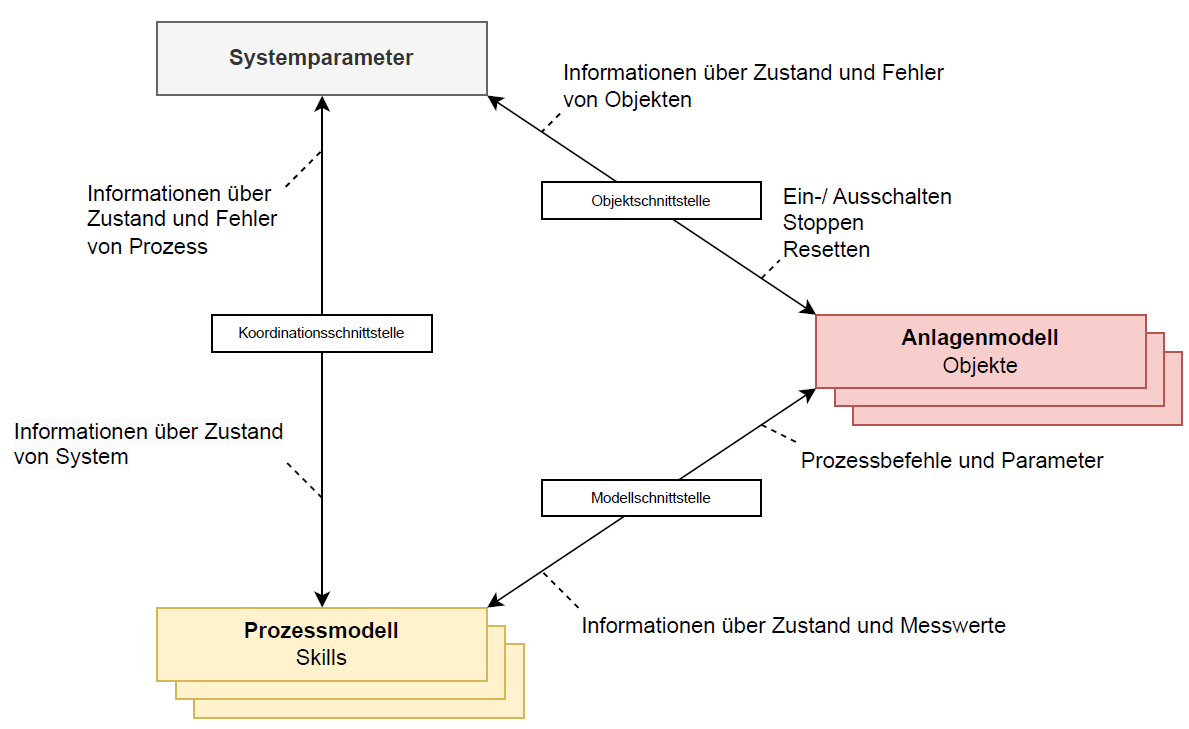
\includegraphics[width=0.6\textwidth]{05_Softwarestruktur/Schnittstellenoverview}
		\captionsetup{justification=centering}
		\caption{Schnittstellenübersicht}
		\label{fig:Schnittstellenübersicht}
	\end{figure}
	
	Die Schnittstellen und deren Abgrenzung dienen als Grundlage für die Bestimmung der Zustände. Dabei werden die Zustände für das System, die Skills und die Objekte bestimmt. Die System- und Objektzustände sind entscheidend für die grundlegende Struktur der Skills, da diese auf die jeweiligen Zustände reagieren müssen. Folglich stellen die definierten System- und Objektzustände lediglich die Mindestanforderungen dar, die notwendig sind, um eine Interaktion mit den Skills zu ermöglichen. Bei der Entwicklung der jeweiligen Systemelemente (Prozessmodell \verb|&| Anlagenmodell) können noch weitere Zustände dazukommen. 
	
	\newpage
	
	\textbf{System:}
	\vspace{2mm} 
	\\
	Das System besitzt mindestens folgende 5 Zustände:
	
	\begin{table}[ht]
		\scriptsize
		\centering
		\colorlet{BFH-table}{BFH-MediumBlue!10}
		\colorlet{BFH-tablehead}{BFH-MediumBlue!50}
		\begin{bfhTabular}{ll}
			Zustand: 		& Beschreibung:															\\\hline
			0 | \verb|AUS| 		& Das System ist ausgeschaltet (Startzustand)							\\\hline
			1 | \verb|BEREIT|	& Das System ist eingeschaltet und bereit einen Prozess durchzuführen	\\\hline
			2 | \verb|LAUFEND| 	& Ein Prozess wird ausgeführt											\\\hline
			3 | \verb|GESTOPPT|	& Ein Prozess wurde gestoppt											\\\hline
			4 | \verb|FEHLER|	& Es gibt einen Fehler im System 
		\end{bfhTabular}
		\captionsetup{justification=centering}
		\caption{Minimale Systemzustände}
		\label{tab:Minimale_Systemzustände}
	\end{table}
	
	\begin{figure}[h!]
		\centering
		\includegraphics[width=0.7\textwidth]{05_Softwarestruktur/Systemzustände}
		\captionsetup{justification=centering}
		\caption{Minimale Systemzustände}
		\label{fig:Minimale_Systemzustände}
	\end{figure}
	
	\textbf{Skill:}
	\vspace{2mm} 
	\\
	Ein Skill besitzt 6 Zustände:
	
	\begin{table}[ht]
		\scriptsize
		\centering
		\colorlet{BFH-table}{BFH-MediumBlue!10}
		\colorlet{BFH-tablehead}{BFH-MediumBlue!50}
		\begin{bfhTabular}{ll}
			Zustand: 			& Beschreibung:															\\\hline
			0 | \verb|BEREIT|		& Der Skill ist bereit einen Prozess auszuführen (Startzustand)			\\\hline
			1 | \verb|LAUFEND| 		& Der Skill führt einen Prozess aus										\\\hline
			2 | \verb|ABGESCHLOSSEN|& Der Prozess wurde abgeschlossen (Durch Objekt)						\\\hline
			3 | \verb|ERREICHT|		& Prozessziel wurde erreicht / Prozess beendet (Durch Skill)   			\\\hline
			4 | \verb|LIMIT|		& Grenzwert wurde überschritten und Prozess wurde abgebrochen 			\\\hline
			5 | \verb|FEHLER|		& Es gibt einen Fehler bezüglich des Prozesses  
		\end{bfhTabular}
		\caption{Minimale Skillzustände}
		\label{tab:Minimale_Skillzustände}
	\end{table}
	
	\begin{figure}[h!]
		\centering
		\includegraphics[width=0.7\textwidth]{05_Softwarestruktur/Skillzustände}
		\captionsetup{justification=centering}
		\caption{Minimale Systemzustände}
		\label{fig:Minimale_Skillzustände}
	\end{figure}
	
	\newpage
	
	\textbf{Objekt:}
	\vspace{2mm} 
	\\
	Ein Objekt benötigt mindestens folgende 7 Zustände:
	
	\begin{table}[ht]
		\scriptsize
		\centering
		\colorlet{BFH-table}{BFH-MediumBlue!10}
		\colorlet{BFH-tablehead}{BFH-MediumBlue!50}
		\begin{bfhTabular}{ll}
			Zustand: 						& Beschreibung:															\\\hline
			0 | \verb|AUS|					& Das Objekt ist ausgeschaltet (Startzustand)							\\\hline
			1 | \verb|BEREIT|				& Das Objekt ist eingeschaltet und bereit								\\\hline
			2 | \verb|LAUFEND| 				& Das Objekt ist aktiv													\\\hline
			3 | \verb|ABGESCHLOSSEN_INTERN|	& Prozess wurde abgeschlossen (Durch Objekt)							\\\hline
			4 | \verb|ABGESCHLOSSEN_EXTERN|	& Prozess wurde abgeschlossen (Durch Skill)								\\\hline
			5 | \verb|GESTOPPT|				& Prozess wurde gestoppt (Durch System)		 							\\\hline
			6 | \verb|FEHLER|				& Es gibt einen Fehler bezüglich des Objektes
		\end{bfhTabular}
		\caption{Minimale Objektzustände}
		\label{tab:Minimale_Objektzustände}
	\end{table}
	
	\begin{figure}[h!]
		\centering
		\includegraphics[width=0.7\textwidth]{05_Softwarestruktur/Objektzustände}
		\captionsetup{justification=centering}
		\caption{Minimale Objektzustände}
		\label{fig:Minimale_Objektzustände}
	\end{figure}
	\vspace{3mm}
	
	Die Definition der allgemeinen Software-Struktur und ihrer Interaktionen bildet die Grundlage für die Ausarbeitung der detaillierten Struktur, Funktionsweise und Implementierung der Skills sowie des Anlagenmodells.
	
	
	

\chapter{Entwicklung der Skills} \label{Entwicklung der Skills}
Die Struktur der Software muss auf einen skill-basierten Ansatz ausgelegt werden. Dafür müssen die Anforderungen an eine solche Struktur klar definiert und die Möglichkeiten, die TwinCAT bietet, analysiert werden. In einem ersten Schritt wird die allgemeine Grobstruktur des Systems dargestellt (Abb. \ref{fig:Strukturübersicht}). Dieses kann wie folgt definiert werden: 

\begin{figure}[h!]
	\centering
	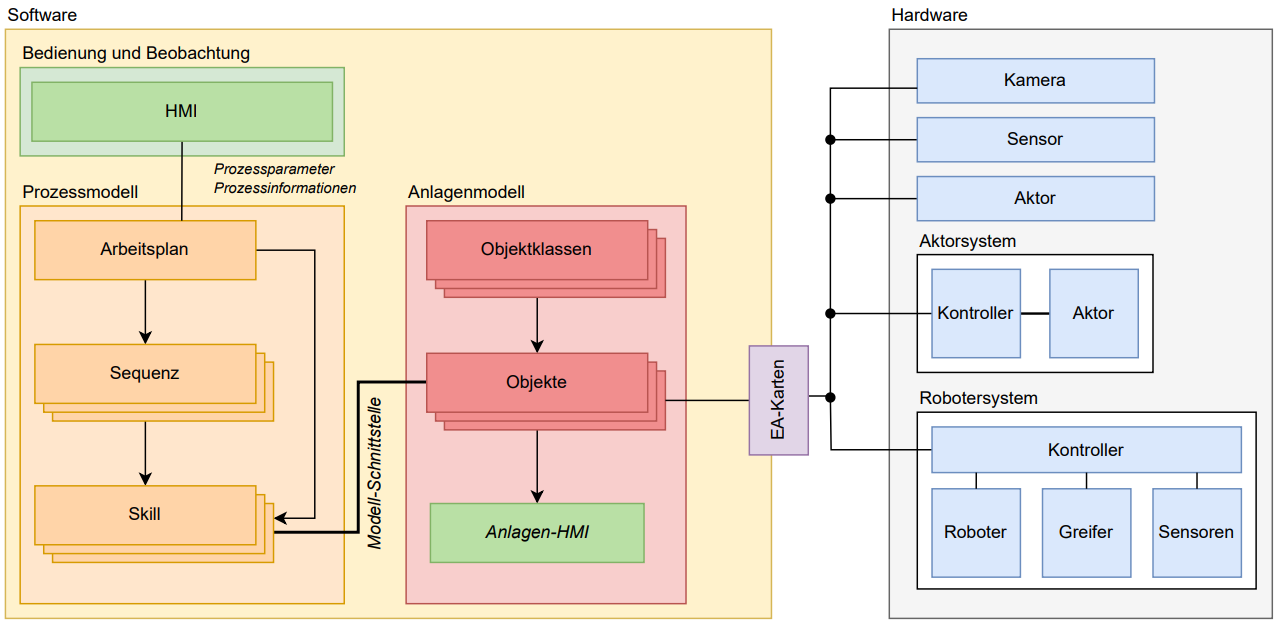
\includegraphics[width=1\textwidth]{05_Softwarestruktur/Overview}
	\captionsetup{justification=centering}
	\caption{Strukturübersicht}
	\label{fig:Strukturübersicht}
\end{figure}

Wie durch die ANSI/ISA-88-Norm vorgegeben (beschrieben in Kapitel \ref{Fragen bezüglich Referenzprojekt}), besteht die Software aus einem Prozess- und einem Anlagenmodell. Das Prozessmodell steuert den Ablauf, während das Anlagenmodell die Schnittstelle zu den einzelnen Anlagenkomponenten darstellt. Innerhalb des Prozessmodells werden die Skills definiert, die entweder von Sequenzen oder direkt aus dem Arbeitsplan zur Ablaufsteuerung genutzt werden können. Der Arbeitsplan beschreibt den gesamten Prozess.
\\
Das Anlagenmodell implementiert die Objektklassen der verschiedenen Systemelemente und bildet deren Funktionalitäten ab. Die Struktur des Anlagenmodells ist klar und übersichtlich: Die Objektklassen werden instanziiert und diese Objekte mit den entsprechenden Ein- und Ausgängen verknüpft, welche die Schnittstelle zum realen System darstellen. Der Grundgedanke dabei ist, dass alle Funktionalitäten zentral in der \Gls{SPS} gebündelt werden, um möglichst wenig Funktionalität auf den einzelnen Komponenten selbst zu belassen. Ziel ist es, dass sämtliche Elemente, von Robotern bis zu Kameras, über die \Gls{SPS} gesteuert werden können. Voraussetzung dafür ist, dass alle Komponenten über eine funktionale Schnittstelle zur \Gls{SPS} verfügen. Alle Komponenten werden im Anlagen-HMI visualisiert und können dort manuell gesteuert werden. Dies ermöglicht es beispielsweise, Roboterpositionen zu speichern, die später von einem Skill für Bewegungsabläufe genutzt werden können. 
\\
Abschliessend gibt es eine Bedienungs- und Beobachtungsebene, die als Benutzerschnittstelle dient, um Prozessparameter einzugeben und Informationen über den Prozess anzuzeigen. Diese Systemstruktur ermöglicht auch den modularen Aufbau von Systemen (Abb. \ref{fig:Gesamtsystemstruktur}). Das folgende Schema zeigt, wie ein solches System aussehen könnte:

\begin{figure}[h!]
	\centering
	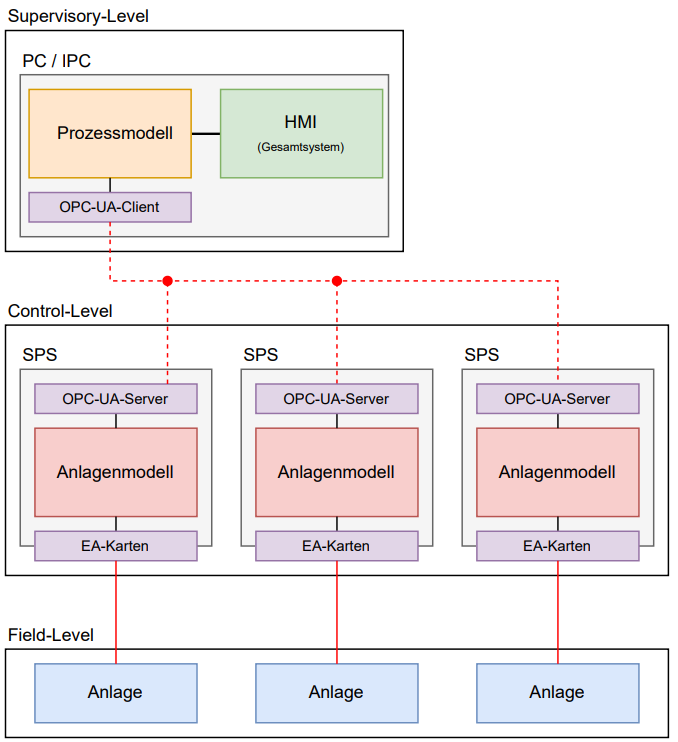
\includegraphics[width=0.5\textwidth]{05_Softwarestruktur/Gesamtsystemstruktur}
	\captionsetup{justification=centering}
	\caption{Gesamtsystemstruktur}
	\label{fig:Gesamtsystemstruktur}
\end{figure}

Das Schema orientiert sich an der Automatisierungspyramide \cite{Automatisierungspyramide} und zeigt die ersten drei Ebenen (Supervisory-, Control- und Field-Level). Dabei handelt es sich um ein System, welches aus verschiedenen Teilanlagen besten, mit eigener \Gls{SPS} und Anlagenmodell. Auf dem Supervisory-Level befindet sich das Prozessmodell. Hier wird über die HMI ein Arbeitsplan ausgewählt / zusammengestellt und gestartet. Eine OPC-UA-Schnittstelle übermittelt die prozessrelevanten Daten an die entsprechende \Gls{SPS} im Control-Level. Die \Gls{SPS} steuert die Anlage im Field-Level basierend auf dem Anlagenmodell. Die verschiedenen Anlagen können flexibel für unterschiedliche Aufgaben genutzt werden oder, falls sie identische Fähigkeiten besitzen, nach Auslastung zugewiesen werden. Dadurch ist das System äusserst flexibel und kann ohne grossen Aufwand erweitert werden.

\section{Kompetenzen von Skills} \label{Skillkompetenzen}
	Für die Definition eines Skills wird nicht die Funktion des Gesamtsystem so weit wie möglich in Teilfunktionalitäten heruntergebrochen, sondern die Funktionalitäten der Komponenten im System. Dabei betrachtet man jeden Komponenten-Typ, so weit wie möglich, einzeln (\ref{fig:Skillintegration}). Der Vorteil dieser Definition ist, dass für neue oder angepasste Systeme dieselben Skills eingesetzt werden können. Ein Robotersystem hat in jeder Anlage die identischen Grundfunktionalitäten und somit Skills. Der Skill ist anwendungsunabhängig. Die aus den Skills erstellten Sequenzen bilden die Funktion der Anwendung ab. Damit unterscheidet sich die Definierung der Skills von vergleichbaren Projekten wie z.B. der bereits durchgeführten Master-Thesis auf Basis von ROS (Ref). Dort haben Skills Funktionalitäten von mehreren Komponenten ineinander kombiniert, wodurch der Skill stärker an das spezifische System gebunden war.
	\begin{figure}[h!]
		\centering
		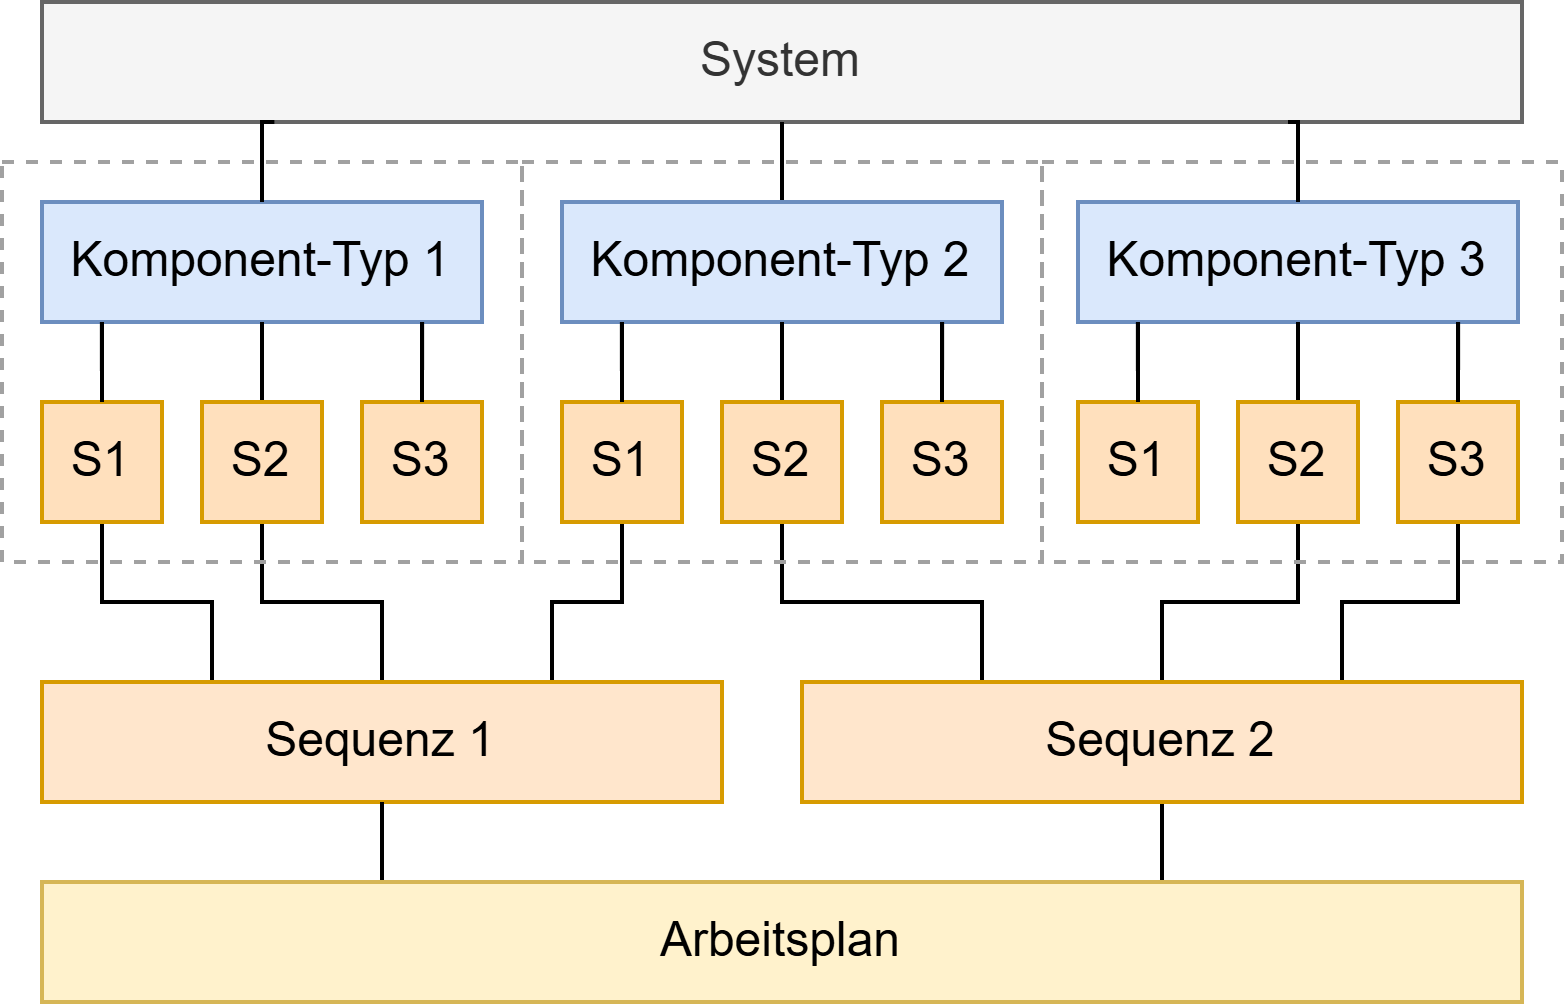
\includegraphics[width=0.7\textwidth]{06_Skillentwicklung/Skillkompetenzen}
		\captionsetup{justification=centering}
		\caption{Skill-Integration in System}
		\label{fig:Skillintegration}
	\end{figure}
	
	Die Kompetenzen eines Skills lassen sich in vier Bereiche aufteilen: 
	
	\begin{tabularx}{\textwidth}{@{}>{}p{8em} X@{}}
		Zuweisung: & 
		Der Skills ist für die Zuweisung einer Komponente zuständig. Es muss definiert werden können, welche Komponente den Skill ausführt.
		\\
		Umsetzung: & 
		Die definierte Grundfunktion muss innerhalb des Skills umgesetzt werden. Der Skill muss mittels Parameter-Inputs flexibel eingesetzt werden können.
		\\
		Verarbeitung: & 
		Die Informationen der Grundfunktion wird so ausgegeben, dass das Anlagenobjekt damit arbeiten und die reale Komponente ansteuern kann.
		\\
		Auswertung: & 
		Die momentane Situation der Komponente wird überwacht und ausgewertet. Der Skill kann auf bestimmte Situationen reagieren. 
		\\
	\end{tabularx}
\section{Definition von Skills für Anwendung} \label{Anwendungsskills}
	Um die benötigten Skills für die Anwendung zu definieren, werden im ersten Schritt die allgemeinen Arbeitsschritte (\ref{tab:Arbeitsschritte}) basierend auf dem mechanischen Aufbau (siehe Verweis) festgelegt. Dabei wird von der Ausgangssituation ausgegangen, dass alle Teile in ihren Lagerpositionen abgelegt sind, der Roboter sich in der Home-Position befindet und alle Komponenten eingeschaltet sowie betriebsbereit sind.
	
	\begin{table}[ht]
		\centering
		\colorlet{BFH-table}{BFH-MediumBlue!10}
		\colorlet{BFH-tablehead}{BFH-MediumBlue!50}
		\begin{bfhTabular}{lll}
			Schritt: 	& Beschreibung:				&Komponente:								
			\\\hline
			1			& Position von Platte 1 in Lagerung erkennen							& K
			\\\hline
			2			& Platte 1 mittels L-Stück ausrichten									& R, G, K
			\\\hline
			3 			& Position von Platte 2 in Lagerung erkennen							& K
			\\\hline
			4			& Platte 2 und  Platte 1 zusammenführen									& R, G, K
			\\\hline
			5			& Position der Befestigungslöcher in den Platten ermitteln				& K
			\\\hline
			6			& Position von Befestigungsblech in Lagerung erkennen		 			& K	
			\\\hline
			7			& Befestigungsblech an Montageposition bringen 							& R, G, K
			\\\hline
			8			& Position von Stift 1 in Lagerung erkennen								& K
			\\\hline
			9			& Stift 1 an korrekte Position bringen									& R, G
			\\\hline
			10			& Befestigungsblech mit Platte 1 verbinden (mit Stift) 					& R, G
			\\\hline
			11			& Wiederholen von Schritt 8 – 10 für Stift 2 bis 3						&
		\end{bfhTabular}
		\begin{tablenotes}
			\small
			\item (K = Kamerasystem | R = Roboter | G = Greifer)
		\end{tablenotes}
		\caption{Arbeitsschritte}
		\label{tab:Arbeitsschritte}
	\end{table}
	
	Eine detaillierte Auflistung der Arbeitsschritte wird im Anhang beigefügt. Aus diesem lässt sich erkennen, dass sich diverse Schritte mit kleinen Anpassungen wiederholen.  Diese sich wiederholenden Arbeitsschritte definierten die Skills. Ein entscheidender Aspekt dabei ist, dass der Roboter und der Kraftsensor als separate Komponenten betrachtet werden. Der Kraftsensor erweitert die Fähigkeiten des Roboters zwar und damit dessen Skills, jedoch kann der Roboter auch ohne Kraftsensor betrieben werden. Der Kraftsensor wird als eigene Objektklasse abgebildet, jedoch besitzt dieser keinen eigenen Skill. Folgende Skills wurden definiert, welche den Prozess abdecken:
	
	\begin{table}[ht]
		\centering
		\colorlet{BFH-table}{BFH-MediumBlue!10}
		\colorlet{BFH-tablehead}{BFH-MediumBlue!50}
		\begin{bfhTabular}{lll}
			Komponenten: 	& Skill:								& Bemerkung:								
			\\\hline
			Kamerasystem			& - Bild aufnehmen				& 
			\\\hline
									& - Objekt erkennen				& 
			\\\hline
									& - Greiferposition ermitteln	& 
			\\\hline
			Roboter					& - Position anfahren			& 
			\\\hline
									& - Kontrolliert bewegen		& Bei Kraftüberschreitung wird gestoppt
			\\\hline
			Greifer (mit Sensor)	& - Backenposition anfahren		& 									
		\end{bfhTabular}
		\begin{tablenotes}
			\small
			\item (Kamerasystem = Kamera + Vision)
		\end{tablenotes}
		\caption{Definierte Skills für Anwendung}
		\label{tab:Definierte_Skills}
	\end{table}
\section{Definierung der Skill-Struktur} \label{Skillstruktur}
	Alle Skills sollten nach einer einheitlichen Struktur aufgebaut sein und lediglich um die prozessspezifischen Funktionen ergänzt werden. Ein zentraler Bestandteil dieser Grundstruktur sind die Schnittstellen, die ein Skill mindestens benötigt, um innerhalb der Systemstruktur funktionsfähig zu sein. Dazu zählen nicht nur Eingangs- und Ausgangsvariablen, sondern auch Eigenschaften und Methoden, da Informationen ebenfalls über diese übertragen werden können. Ein Skill muss über die definierten Schnittstellen (siehe Kapitel \ref{Softwareinteraktion}) sowohl mit dem System, mit dem Objekt und innerhalb des Prozessmodells interagieren können. 
	\\
	Innerhalb der Entwicklung wurden mehrere Iterationen von Skill-Strukturen geplant, umgesetzt und getestet, um die bestmöglichste Struktur zu finden. Innerhalb dieser Dokumentation werden nicht alle Iterationsschritte erklärt, sondern nur die daraus folgenden Erkenntnisse. 
	\\
	Die Schnittstellen eines Skills wurden in folgende drei Kategorien aufgeteilt, welche das allgemeine Verständnis einfacher machen sollen.
	
	\textbf{Steuerungselemente:}
	\vspace{2mm} 
	\\
	Die Steuerungselemente sind für die Bedienung des Skills angedacht. Hier wird der Skill gestartet, gestoppt oder resettet. Zusätzlich werden auch Informationen über den Zustand des Skills angegeben.
	
	\textbf{Betriebselemente:}
	\vspace{2mm} 
	\\
	Die Betriebselemente sind für den allgemeinen Betrieb des Skills angedacht, welche nicht mit dem spezifischen Prozess zu tun haben. Dies ist z.B. die Schnittstelle zum System, welche eine Aussage über den Systemzustand macht. 
	
	\textbf{Prozesselemente:}
	\vspace{2mm} 
	\\
	Die Prozesselemente sind spezifische Informationen, welche der Skill für die Ausführung benötigt und entsprechend  an das Objekt weitergibt. 
	\vspace{5mm} 
	
	Zu Beginn wurden die Steuerungselemente auf Basis des PLC-Standards aufgebaut (beschrieben in Kapitel \ref{Marktanalyse}). Der Skill wurde dabei von einer \verb|BOOL|-Variable (\verb|bExecute|) gestartet und hat diverse Informationen als Ausgangsvariablen ausgegeben (\verb|bDone|, \verb|bBusy|, \verb|bLimit|, \verb|bError| und \verb|iErrorID|). Die Ausgangsvariablen konnten als Transition-Bedingungen für Abläufe verwendet werden. Auf den ersten Blick ist dies eine einfache und sinnvolle Steuerung des Skills. Jedoch zeigte sich bei ersten Versuchen, dass diese Implementierung diverse Probleme mit sich bringen kann. Die Umsetzung eines \verb|bExecute|-Triggers ist aufwändig und muss gut durchdacht werden, da der Skill nur einmal ausgeführt werden soll. Wenn der Skill beendet wurde und die \verb|bExecute|-Variable immer noch betätigt ist, soll der Skill nicht ein zweites Mal gestartet werden. Der Trigger muss entsprechend so umgesetzt werden, dass dieser nur auf eine steigende Flanke reagiert. Das Management der Ausgangsvariablen ist geknüpft an die verschiedenen Zustände innerhalb des Skills. Es muss genau bestimmt werden, welcher Zustand einen Einfluss auf die Ausgänge hat. Durch die hohe Anzahl an Ausgangsvariablen kann man hierbei schnell den Überblick verlieren. Zusätzlich werden viele der Informationen, welche über die Ausgangsvariablen dargestellt werden, auch über den Zustand dargestellt. Die Konsequenz daraus ist, dass die Steuerungselemente mit Methoden und Eigenschaften umgesetzt werden (Tab. \ref{tab:Skill_Steuerungselemente}). 
	
	\newpage
	
	\begin{table}[ht]
		\centering
		\colorlet{BFH-table}{BFH-MediumBlue!10}
		\colorlet{BFH-tablehead}{BFH-MediumBlue!50}
		\begin{bfhTabular}{llcl}
			Art: 		& Bezeichnung:		& Typ:				& Beschreibung:								
			\\\hline
			Methode		& \verb|M_Start|	& \verb|BOOL|		& Methode zum Starten des Skills
			\\\hline
			Methode		& \verb|M_Stop|		& \verb|BOOL|		& Methode zum Stoppen des Skills
			\\\hline
			Methode		& \verb|M_Reset|	& \verb|BOOL|		& Methode zum Resetten des Skills
			\\\hline
			Eigenschaft	& \verb|P_State|	& \verb|eSkillState|& Eigenschaft des aktuellen Zustandes
		\end{bfhTabular}
		\captionsetup{justification=centering}
		\caption{Steuerungselemente eines Skills}
		\label{tab:Skill_Steuerungselemente}
	\end{table}
	
	 Die Eigenschaft wird mit einem benutzerdefinierten \verb|ENUM|-Datentyp umgesetzt (Tab. \ref{tab:eSkillState}), welche die Zustände des Skills abbildet. Somit ist immer klar, in welchem Zustand sich der Skill im Moment befindet. 
	 
	 \begin{table}[ht]
	 	\centering
	 	\colorlet{BFH-table}{BFH-MediumBlue!10}
	 	\colorlet{BFH-tablehead}{BFH-MediumBlue!50}
	 	\begin{bfhTabular}{cc}
	 		Listen-Nr: 		& eSkillState:									
	 		\\\hline
	 		0				& \verb|BEREIT|	
	 		\\\hline
	 		1				& \verb|LAUFEND|		
	 		\\\hline
	 		2				& \verb|ABGESCHLOSSEN|		
	 		\\\hline
	 		3				& \verb|FEHLER|	
	 		\\\hline
	 		4				& \verb|LIMIT|	
	 		\\\hline
	 		5				& \verb|ERREICHT|	
	 	\end{bfhTabular}
	 	\captionsetup{justification=centering}
	 	\caption{Definition von eSkillState}
	 	\label{tab:eSkillState}
	 \end{table}
	 
	 Auch bei den Betriebselementen gab es im Verlauf der Entwicklung Veränderungen. Zu Beginn enthielten diese alle Variablen, die für den Betrieb des Skills erforderlich waren und dienten als Schnittstelle zwischen System und Objekt. Relevante Informationen für den Prozess wurden dabei über Ausgangsvariablen an das Objekt übergeben, welches diese wiederum als Eingangsvariablen entgegennahm.
	 \\
	 Wenn jedoch zwei Skills auf dasselbe Objekt zugreifen sollen (nicht gleichzeitig) und beide mit dessen Eingangsvariablen verbunden sind, überschreibt stets einer der beiden Skills den Wert des anderen. Da es durchaus vorkommt, dass mehrere Skills mit einem Objekt interagieren (ebenfalls nicht gleichzeitig), muss die Interaktion zwischen Skill und Objekt so gestaltet sein, dass sie unabhängig von anderen Skills funktioniert.
	 \\
	 \begin{wrapfigure}{r}{0.45\textwidth}
	 	\centering
	 	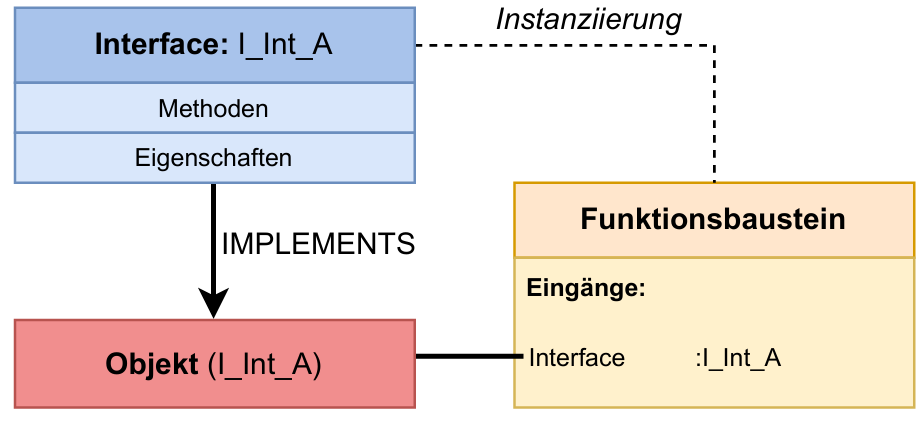
\includegraphics[width=0.45\textwidth]{06_Skillentwicklung/Schnittstellenstruktur}
	 	\captionsetup{justification=centering}
	 	\caption{Schnittstellenstruktur}
	 	\label{fig:Schnittstellenstruktur}
	 \end{wrapfigure} Dies lässt sich durch die Instanziierung eines Interfaces erreichen. In der objektorientierten Programmierung wird ein Interface genutzt, um vorzugeben, welche Methoden und Eigenschaften ein Funktionsbaustein zwingend besitzen muss. Durch das Instanziieren eines Interfaces innerhalb eines Funktionsbausteins können dessen Methoden und Eigenschaften verwendet werden. Wenn eine Eingangsvariable mittels Interface instanziiert wird, kann diese Funktionsbaustein-Eingangsvariable mit einem Objekt verbunden werden, insofern das selbe Interface beim Objekt implementiert wurde (Abb. \ref{fig:Schnittstellenstruktur}). Beim Ausführen einer Methode innerhalb des Funktionsbausteins wird dadurch die entsprechende Methode im verknüpften Objekt aufgerufen. Gleiches gilt für die Eigenschaften. Dadurch kann z.B. der Zustand des Objektes über diese Schnittstelle abgefragt werden. 
	 
	 \newpage
	 
	 Somit wurden die Betriebselemente wie folgt definiert: 
	 
	 \begin{table}[ht]
	 	\centering
	 	\colorlet{BFH-table}{BFH-MediumBlue!10}
	 	\colorlet{BFH-tablehead}{BFH-MediumBlue!50}
	 	\begin{bfhTabular}{llcl}
	 		Art: 				& Bezeichnung:		& Typ:						& Beschreibung:								
	 		\\\hline
	 		Eingangsvariabel	& \verb|eSysCommand|& \verb|eSystemCommand|		& Befehl von System zu Skill
	 		\\\hline
	 		Eingangsvariabel	& \verb|eSysState|	& \verb|eSystemStatus|		& Informationen über System 
	 		\\\hline
	 		Eingangsvariabel	& \verb|fbObjekt|	& Objekt-Interface			& Verknüpfung zu Objekt
	 		\\\hline
	 		Ausgangsvariabel	& \verb|iErrorID|	& \verb|INT|				& Information über Fehler
	 	\end{bfhTabular}
	 	\caption{Betriebselemente eines Skills}
	 	\label{tab:Skill_Betriebselemente}
	 \end{table}
	 
	 Da auch die Übergabe der Objektparameter an das Objekt über die Interface-Verknüpfung erfolgt (mittels einer Eigenschaft), wird für jede Art von Objekttyp ein eigenes Interface definiert, da Objekte unterschiedliche Parameter benötigen. Die Steuerungselemente für ein Objekt sind jedoch für alle Objekttypen einheitlich und ähnlich wie bei den Skills. Dazu gehören die Methoden «\verb|M_Start|», «\verb|M_Stop|», «\verb|M_Rest|» sowie die Eigenschaft «\verb|P_State|» (ObjectState).
	 \\
	 Die folgenden benutzerdefinierten Datentypen sind für die Betriebselemente von Bedeutung:
	 
	  \begin{table}[ht]
	 	\centering
	 	\colorlet{BFH-table}{BFH-MediumBlue!10}
	 	\colorlet{BFH-tablehead}{BFH-MediumBlue!50}
	 	\begin{bfhTabular}{cccc}
	 		Listen-Nr: 	& \verb|eSystemCommand|:	& \verb|ObjectState|:	& \verb|eSystemState|:									
	 		\\\hline
	 		0			& \verb|KEINE|		& \verb|AUS|					& \verb|AUS| 
	 		\\\hline
	 		1			& \verb|AUSSCHALTEN|& \verb|BEREIT|					& \verb|BEREIT|
	 		\\\hline
	 		2			& \verb|EINSCHALTEN|& \verb|MANUELL|				& \verb|LAUFEND|
	 		\\\hline
	 		3			& \verb|STOPPEN|	& \verb|LAUFEND|				& \verb|GESTOPPT|
	 		\\\hline
	 		4			& \verb|RESETTEN|	& \verb|ABGESCHLOSSEN_INTERN|	& \verb|FEHLER|
	 		\\\hline
	 		5			& \verb|/|			& \verb|ABGESCHLOSSEN_EXTERN|	& \verb|/|
	 		\\\hline
	 		6			& \verb|/|			& \verb|GESTOPPT|				& \verb|/|
	 		\\\hline
	 		7			& \verb|/|			& \verb|FEHLER|					& \verb|/|
	 	\end{bfhTabular}
	 	\captionsetup{justification=centering}
	 	\caption{Benutzerdefinierte Datentypen}
	 	\label{tab:Datentypen_Benutzerdefiniert}
	 \end{table}
	 
	 \begin{bfhNoteBox}
	 	Beim Datentyp «\verb|ObjectState|» wird unterschieden zwischen einem Aktor oder einem Sensor. Die dargestellten Zustände beziehen sich auf einen Aktor. Innerhalb von Kaptiel \ref{Entwicklung des Anlagenmodells} wird detaillierter auf den Unterschied zwischen Aktoren und Sensoren eingegangen. 
	 \end{bfhNoteBox}
	 \vspace{3mm}
	 
	 Die letzte Kategorie umfasst die Prozesselemente. Die Prozesseigenschaften dienen dem bereitstellen von prozessrelevanten Informationen. Die vorhandenen Prozessmethoden werden vom Skill intern genutzt, beispielsweise zur Datenverarbeitung oder  Auswertung.
	 
	 \newpage
	 
	 Die Grundstruktur eines Skills lässt sich anhand des folgenden Schemas zusammenfassen (Abb. \ref{fig:Skillschnittstellen}). Dieses Schema veranschaulicht auch die Interaktion des Skills über die verschiedenen Schnittstellen im System.
	 \\
	 \begin{figure}[h!]
	 	\centering
	 	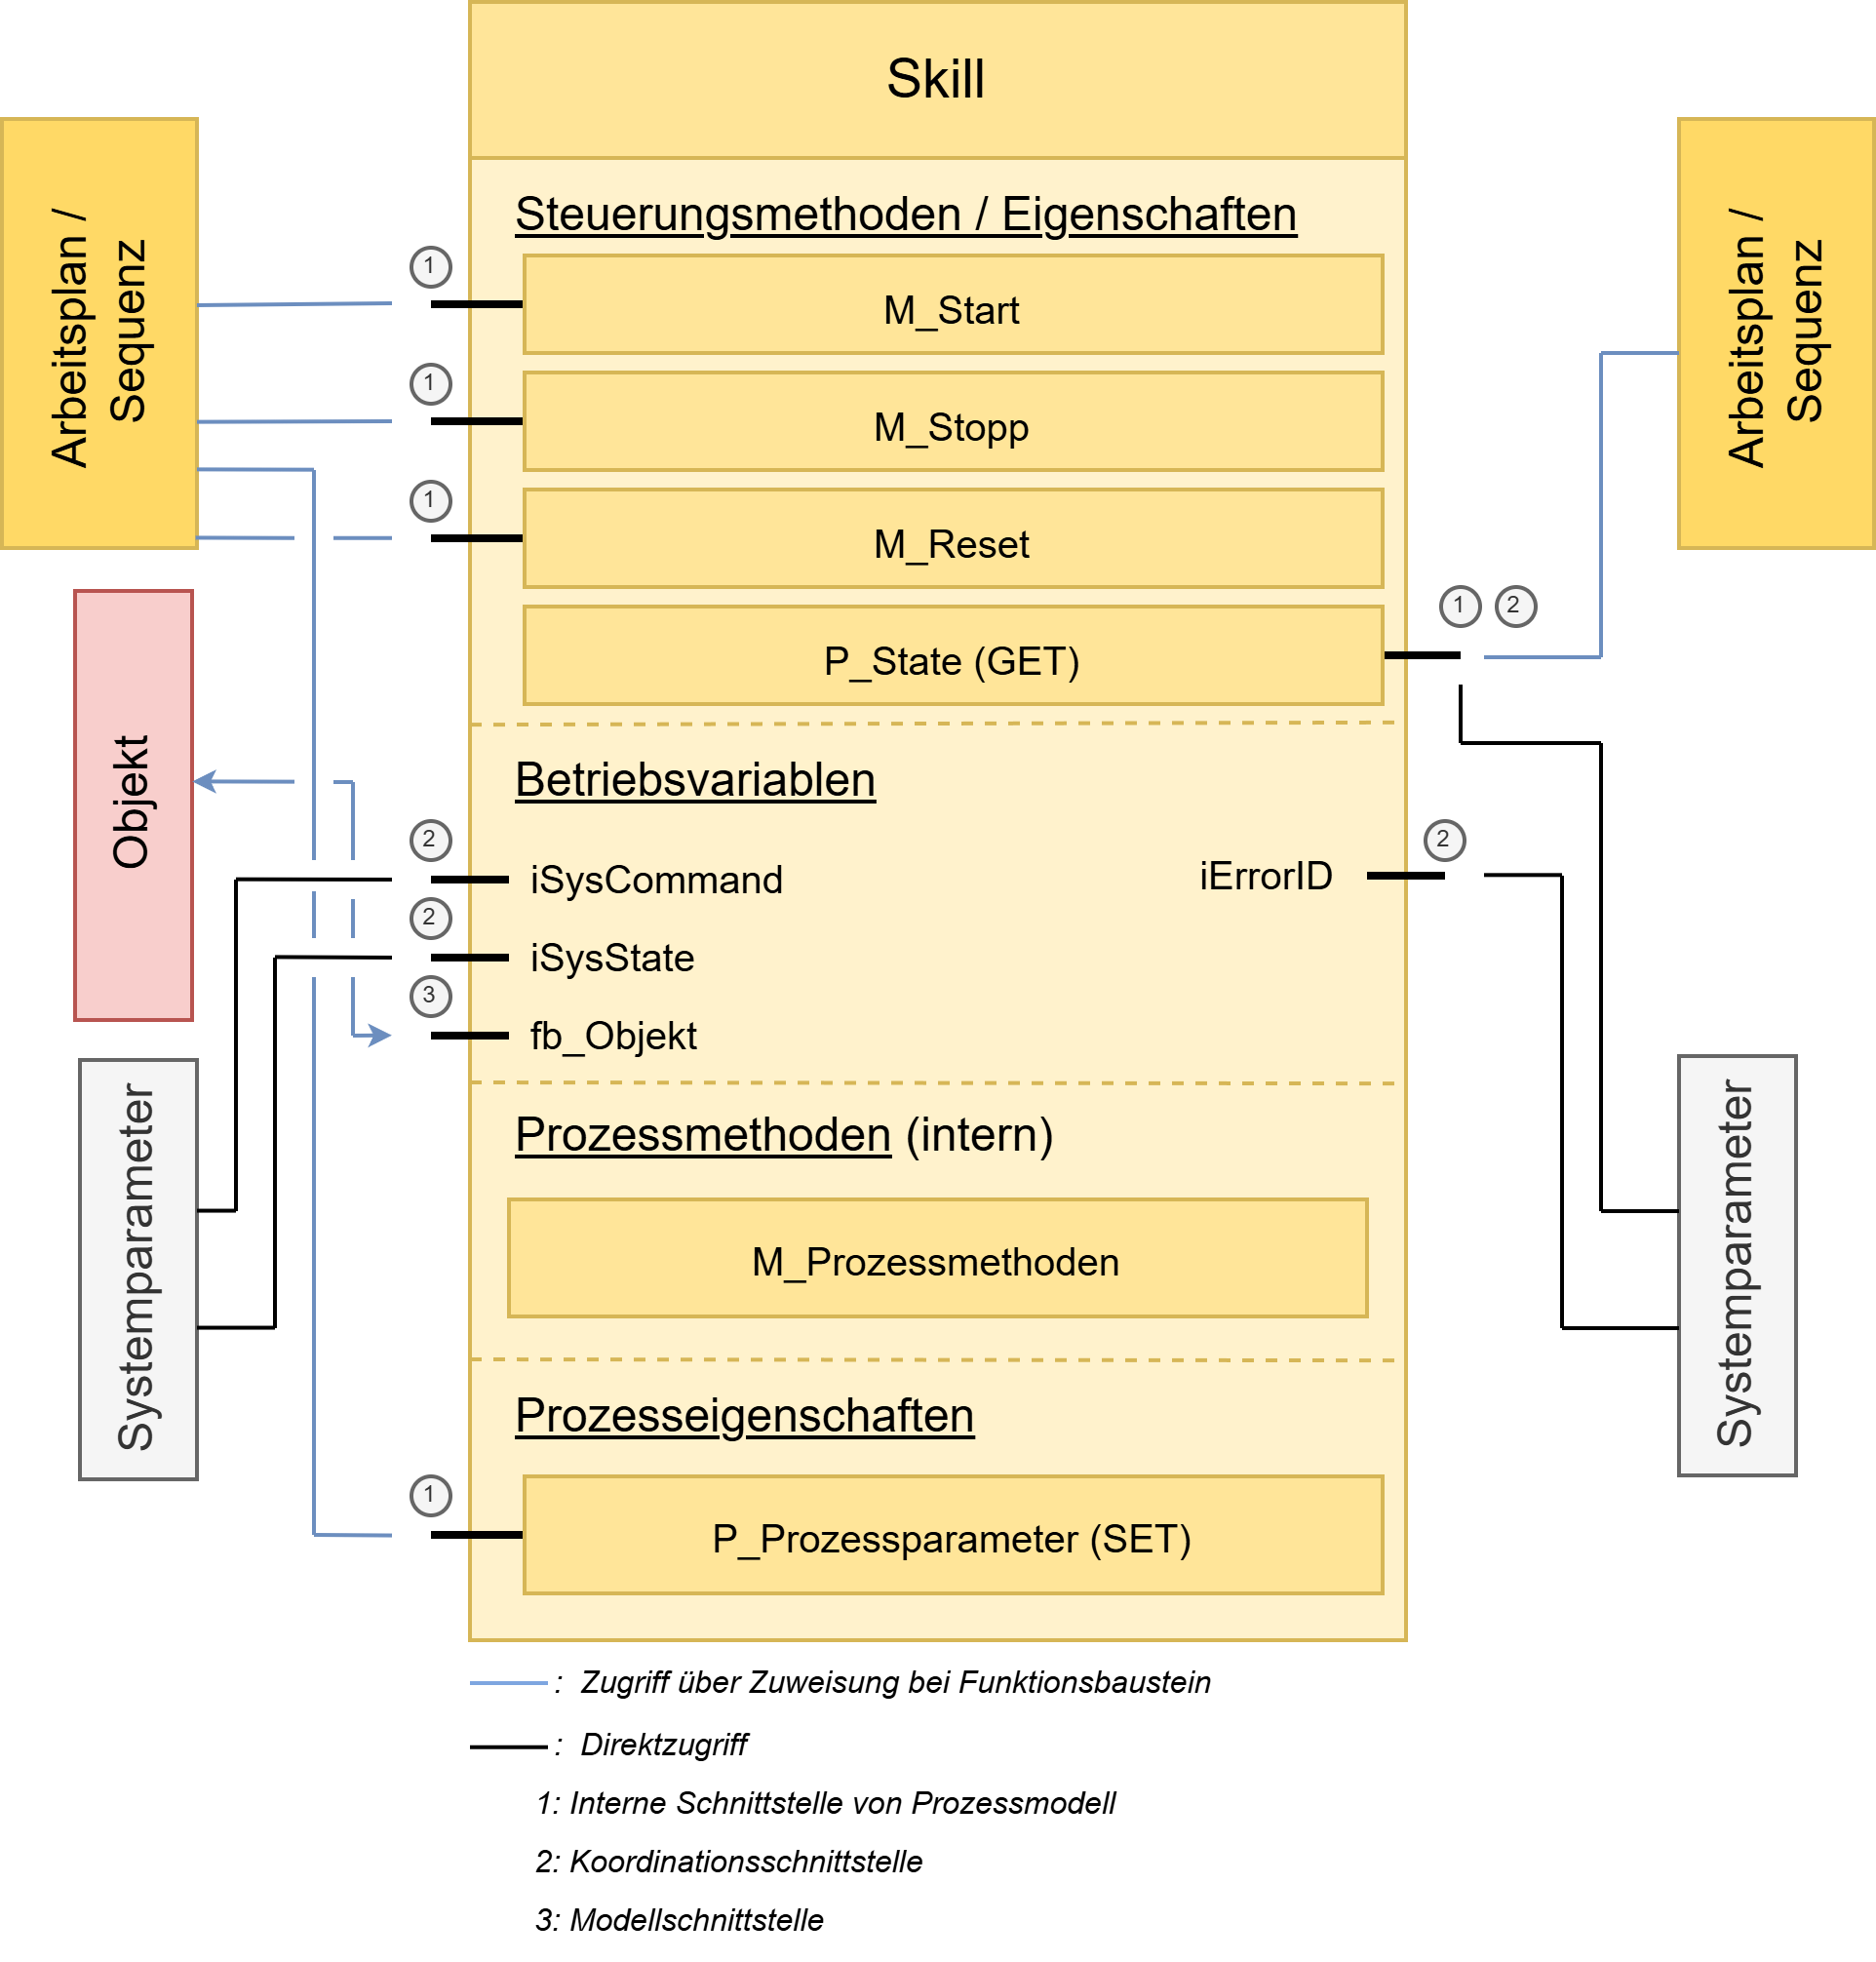
\includegraphics[width=1\textwidth]{06_Skillentwicklung/Skillschnittstellen}
	 	\captionsetup{justification=centering}
	 	\caption{Skilldefinition und Schnittstellen}
	 	\label{fig:Skillschnittstellen}
	 \end{figure}
	 
	 \newpage
	 
	 
\section{Konfiguration eines Skills} \label{Skillkonfiguration}
	Nicht jeder Skill benötigt alle Zustände. Damit der Skill so übersichtlich wie möglich bleibt, sollen auch nur die Zustände verwendet werden, welche benötigt werden. Ein Skill kann drei Konfigurationen einnehmen (Abb. \ref{fig:Skillkonfiguration}).
	\\
	\begin{figure}[h!]
		\centering
		\includegraphics[width=0.8\textwidth]{06_Skillentwicklung/Skillkonfiguration}
		\captionsetup{justification=centering}
		\caption{Skillkonfiguration}
		\label{fig:Skillkonfiguration}
	\end{figure}
	
	\begin{tabularx}{\textwidth}{@{}>{}p{8em} X@{}}
		Konfiguration 1: & 
		Stellt die Grundkonfiguration dar. Jeder Skill muss diese Zustände implementieren. Hierbei handelt es sich um Skills, welche nur durch das Objekt abgeschlossen werden, z.B. eine einfache Punkt-Zu-Punkt-Bewegung des Roboters.
		\\
		Konfiguration 2: & 
		Bei dieser Konfiguration kommt der \verb|LIMIT|-Zustand dazu. Dieser wird benötigt, wenn es eine Limit-Bedingung gibt, z.B. einen Grenzwert für die Kraft oder eine maximale Zeitdauer.
		\\
		Konfiguration 3: & 
		Bei der letzten Konfiguration wird der \verb|ERREICHT|-Zustand ergänzt. Dieser gibt an, ob ein definiertes Ziel erreicht wurde, dies kann z.B. eine Kraft sein.
		\\
	\end{tabularx}
\section{Interaktion zwischen Skill und Objekt} \label{SkillObjektInteraktion}
	Anhand eines Beispiels (\ref{fig:Skillinteraktion}) soll die Interaktion zwischen einem Skill und den zugehörigen Objekten erläutert werden. Der Skill «\verb|Skill_P2P|» ermöglicht es einem Roboter, zu einem definierten Punkt zu fahren. Falls der Roboter dabei mit einem Hindernis kollidiert, wird der Roboter durch den Skill gestoppt. Hindernisse werden dabei mithilfe eines Kraftsensors erkannt.
	\\
	Der Skill wird über Eingangsvariablen mit den entsprechenden Objekten verbunden, was durch eine blaue Verbindungslinie dargestellt wird. Über die Sequenz werden verschiedene Informationen an den Skill übergeben. Dazu zählen:
	\begin{itemize}
		\item Die aktuelle Position des Roboters
		\item Die Geschwindigkeit und Beschleunigung
		\item Die Art der Bewegung bzw. Positionierung
		\item Die Kraftgrenze, die ein Hindernis definiert
	\end{itemize}
	
	Der Start des Skills erfolgt durch die Start-Methode, die von der Sequenz ausgelöst wird. Der Skill selbst initiiert über die Start-Methode des Aktor-Objekts den Bewegungsprozess und liest parallel dazu mithilfe der Messdaten-Eigenschaft die Daten des Sensor-Objekts aus. Die Objekte haben dabei ausschliesslich der Aufgabe, ihre spezifischen Funktionen auszuführen, die durch ihre jeweilige Komponente definiert sind. Sie enthalten keine Logik in Bezug auf das Gesamtsystem – diese liegt vollständig im Skill.
	\\
	Der Skill analysiert die übermittelten Daten und reagiert entsprechend darauf. Im geschilderten Beispiel stoppt der Skill den Aktor, sobald die gemessenen Daten die vorgegebenen Schwellenwerte überschreiten.
	
	\begin{figure}[h!]
		\centering
		\includegraphics[width=1\textwidth]{06_Skillentwicklung/Skillinteraktion}
		\captionsetup{justification=centering}
		\caption{Skill-Interaktion}
		\label{fig:Skillinteraktion}
	\end{figure}
	
	\newpage
	
	
	
Text

\chapter{Entwicklung des Anlagenmodells} \label{Entwicklung des Anlagenmodells}
Die Struktur der Software muss auf einen skill-basierten Ansatz ausgelegt werden. Dafür müssen die Anforderungen an eine solche Struktur klar definiert und die Möglichkeiten, die TwinCAT bietet, analysiert werden. In einem ersten Schritt wird die allgemeine Grobstruktur des Systems dargestellt (Abb. \ref{fig:Strukturübersicht}). Dieses kann wie folgt definiert werden: 

\begin{figure}[h!]
	\centering
	\includegraphics[width=1\textwidth]{05_Softwarestruktur/Overview}
	\captionsetup{justification=centering}
	\caption{Strukturübersicht}
	\label{fig:Strukturübersicht}
\end{figure}

Wie durch die ANSI/ISA-88-Norm vorgegeben (beschrieben in Kapitel \ref{Fragen bezüglich Referenzprojekt}), besteht die Software aus einem Prozess- und einem Anlagenmodell. Das Prozessmodell steuert den Ablauf, während das Anlagenmodell die Schnittstelle zu den einzelnen Anlagenkomponenten darstellt. Innerhalb des Prozessmodells werden die Skills definiert, die entweder von Sequenzen oder direkt aus dem Arbeitsplan zur Ablaufsteuerung genutzt werden können. Der Arbeitsplan beschreibt den gesamten Prozess.
\\
Das Anlagenmodell implementiert die Objektklassen der verschiedenen Systemelemente und bildet deren Funktionalitäten ab. Die Struktur des Anlagenmodells ist klar und übersichtlich: Die Objektklassen werden instanziiert und diese Objekte mit den entsprechenden Ein- und Ausgängen verknüpft, welche die Schnittstelle zum realen System darstellen. Der Grundgedanke dabei ist, dass alle Funktionalitäten zentral in der \Gls{SPS} gebündelt werden, um möglichst wenig Funktionalität auf den einzelnen Komponenten selbst zu belassen. Ziel ist es, dass sämtliche Elemente, von Robotern bis zu Kameras, über die \Gls{SPS} gesteuert werden können. Voraussetzung dafür ist, dass alle Komponenten über eine funktionale Schnittstelle zur \Gls{SPS} verfügen. Alle Komponenten werden im Anlagen-HMI visualisiert und können dort manuell gesteuert werden. Dies ermöglicht es beispielsweise, Roboterpositionen zu speichern, die später von einem Skill für Bewegungsabläufe genutzt werden können. 
\\
Abschliessend gibt es eine Bedienungs- und Beobachtungsebene, die als Benutzerschnittstelle dient, um Prozessparameter einzugeben und Informationen über den Prozess anzuzeigen. Diese Systemstruktur ermöglicht auch den modularen Aufbau von Systemen (Abb. \ref{fig:Gesamtsystemstruktur}). Das folgende Schema zeigt, wie ein solches System aussehen könnte:

\begin{figure}[h!]
	\centering
	\includegraphics[width=0.5\textwidth]{05_Softwarestruktur/Gesamtsystemstruktur}
	\captionsetup{justification=centering}
	\caption{Gesamtsystemstruktur}
	\label{fig:Gesamtsystemstruktur}
\end{figure}

Das Schema orientiert sich an der Automatisierungspyramide \cite{Automatisierungspyramide} und zeigt die ersten drei Ebenen (Supervisory-, Control- und Field-Level). Dabei handelt es sich um ein System, welches aus verschiedenen Teilanlagen besten, mit eigener \Gls{SPS} und Anlagenmodell. Auf dem Supervisory-Level befindet sich das Prozessmodell. Hier wird über die HMI ein Arbeitsplan ausgewählt / zusammengestellt und gestartet. Eine OPC-UA-Schnittstelle übermittelt die prozessrelevanten Daten an die entsprechende \Gls{SPS} im Control-Level. Die \Gls{SPS} steuert die Anlage im Field-Level basierend auf dem Anlagenmodell. Die verschiedenen Anlagen können flexibel für unterschiedliche Aufgaben genutzt werden oder, falls sie identische Fähigkeiten besitzen, nach Auslastung zugewiesen werden. Dadurch ist das System äusserst flexibel und kann ohne grossen Aufwand erweitert werden.

\section{Definition der Objekt-Struktur} \label{Objektstruktur}

	Wie bereits für die Skills wird auch für die Objekte eine Grundstruktur festgelegt, die als Basis für den Aufbau aller Objekte dient. Diese einheitliche Struktur erleichtert die Standardisierung der Interaktionen innerhalb der Software. Dabei sollen die Objektklassen möglichst objektorientiert gestaltet werden, sodass die Funktionalität der Objekte in klar abgegrenzten Methoden abgebildet wird. Zum Ausführen einer Funktionalität reicht es daher, die entsprechende Methode aufzurufen. 
	\\
	Die Objekte wurden zusammen mit dem Skills iterativ erarbeitet. Änderungen bei der Skill-Struktur hatten auch einen Einfluss auf die Objektstruktur. 
	\\
	Die Schnittstellen eines Objektes wurden in 4 Kategorien aufgeteilt, welche ähnlich wie beim Skill definiert wurden (siehe Kapitel \ref{Skillstruktur}) und entsprechend das allgemeine Verständnis einfacher machen sollen. 
	
	\textbf{Objektvariablen:}
	\vspace{2mm} 
	\\
	Die Objektvariablen umfassen die Eingangsvariablen (Objektparameter) und die Ausgangsvariablen (Anlagenparameter), welche für den Betrieb des Objektes benötigt werden. Dabei kann es sich z.B. um eine IP-Adresse handeln, wenn das Objekt über eine TCP/IP-Schnittstelle angesprochen wird. Falls das Objekt direkt mit E/A-Klemmen interagieren muss, kann dies über die Anlagenparameter gemacht werden. 
	
	
	\textbf{Steuerungselemente:}
	\vspace{2mm} 
	\\
	Die Steuerungselemente sind für die Bedienung des Objektes angedacht. Hier wird das Objekt gestartet, gestoppt oder resettet. Zusätzlich werden auch Informationen über den Zustand des Objektes angegeben.
	
	
	\textbf{Betriebselemente:}
	\vspace{2mm} 
	\\
	Die Betriebselemente sind für den allgemeinen Betrieb des Objekts angedacht, welche nicht mit dem spezifischen Prozess zu tun haben. Dies ist z.B. die Schnittstelle zum System, welche eine Aussage über Systemzustand macht.
	
	
	\textbf{Prozesselemente:}
	\vspace{2mm} 
	\\
	Die Prozesselemente sind spezifische Informationen, welche das Objekt für die Ausführung benötigt.
	
	Die Steuerungs-, Betriebs- und Prozesselemente erfüllen somit die gleichen Aufgaben wie beim Skill. Zwischen der Struktur von Objekten und Skills gibt es bewusste Parallelen, welche die Verständlichkeit und Übersicht der Gesamtsoftware verbessern sollen. Die Steuerungselemente umfassen die gleichen Methoden und Eigenschaften wie die Skills (Tab. \ref{tab:Objekt_Steuerungselemente}) (Umsetzung dieser unterscheidet sich jedoch). 
	
	\newcolumntype{L}[1]{>{\raggedright\let\newline\\\arraybackslash\hspace{0pt}}m{#1}}
	\begin{table}[ht]
		\centering
		\colorlet{BFH-table}{BFH-MediumBlue!10}
		\colorlet{BFH-tablehead}{BFH-MediumBlue!50}
		\begin{bfhTabular}{| l | l | L{3.7cm} | L{5cm} |}
			Art: 		& Bezeichnung:		& Typ:		& Beschreibung:								
			\\\hline
			Methode		& \verb|M_Start|	& \verb|BOOL|			& Methode zum Starten des Objektes
			\\\hline
			Methode		& \verb|M_Stop|		& \verb|BOOL|			& Methode zum Stoppen des Objektes
			\\\hline
			Methode		& \verb|M_Reset|	& \verb|BOOL|			& Methode zum Resetten des Objektes
			\\\hline
			Eigenschaft	& \verb|P_State|	& \verb|eObjectAktorState| / \verb|eObjectSensorState| & Eigenschaft des aktuellen Zustandes
		\end{bfhTabular}
		\captionsetup{justification=centering}
		\caption{Steuerungselemente eines Objektes}
		\label{tab:Objekt_Steuerungselemente}
	\end{table}
	
	Die Eigenschaft wird mit einem benutzerdefinierten \verb|ENUM|-Datentyp (Tab. \ref{tab:Datentypen_Benutzerdefiniert_Objekt}) umgesetzt, welcher die Zustände des Objektes abbildet. Somit ist immer klar, in welchem Zustand sich das Objekt im Moment befindet. Dabei unterscheidet man zwischen Aktor und Sensor. 
	
	\begin{table}[ht]
		\centering
		\colorlet{BFH-table}{BFH-MediumBlue!10}
		\colorlet{BFH-tablehead}{BFH-MediumBlue!50}
		\begin{bfhTabular}{ccc}
			Listen-Nr: 	& \verb|eObjectAktorState|:		& \verb|eObjectSensorState|:				
			\\\hline
			0			& \verb|AUS|					& \verb|AUS| 
			\\\hline
			1			& \verb|BEREIT|					& \verb|LAUFEND|
			\\\hline
			2			& \verb|MANUELL|				& \verb|FEHLER|
			\\\hline
			3			& \verb|LAUFEND|				& \verb|/|
			\\\hline
			4			& \verb|ABGESCHLOSSEN_INTERN|	& \verb|/|
			\\\hline
			5			& \verb|ABGESCHLOSSEN_EXTERN|	& \verb|/|
			\\\hline
			6			& \verb|GESTOPPT|				& \verb|/|
			\\\hline
			7			& \verb|FEHLER|					& \verb|/|
		\end{bfhTabular}
		\captionsetup{justification=centering}
		\caption{Benutzerdefinierte Objekt-Datentypen}
		\label{tab:Datentypen_Benutzerdefiniert_Objekt}
	\end{table}
	
	In Kapitel \ref{Softwareinteraktion} (Struktur) wurden die Zustände eines Objekts definiert. Dies stellte einen wichtigen Schritt dar, um die allgemeine Interaktion zwischen System, Skill und Objekt festzulegen. Basierend auf diesen Zuständen wurden die finalen Zustände eines Objekts spezifiziert (Abb. \ref{fig:Objektzustände}).
	\\
	Ein Aktor-Objekt erweitert diese Zustände um einen zusätzlichen Zustand für den manuellen Betrieb. Ein Sensor-Objekt hingegen kann  einfacher gestaltet werden: Sobald das System eingeschaltet wird, ist der Sensor aktiv. Dieser Zustand wird nur durch das Ausschalten des Systems oder das Auftreten eines Fehlers verlassen.
	
		\newpage
	
	\begin{figure}[h!]
		\centering
		\includegraphics[width=0.8\textwidth]{07_Anlagenmodell/Objektzustände}
		\captionsetup{justification=centering}
		\caption{Objektzustände}
		\label{fig:Objektzustände}
	\end{figure}
	
	Auch in der Struktur unterscheiden sich Aktor- und Sensor-Objekte geringfügig. Sensor-Objekte verfügen über keine Steuerungsmethoden wie Start, Stopp oder Reset. Stattdessen werden diese Funktionen vom System über die Betriebsvariablen gesteuert.
	Beide Objekt-Typen verwenden jedoch dieselben Betriebsvariablen:
	
	\begin{table}[ht]
		\centering
		\colorlet{BFH-table}{BFH-MediumBlue!10}
		\colorlet{BFH-tablehead}{BFH-MediumBlue!50}
		\begin{bfhTabular}{clcl}
			Art: 				& Bezeichnung:			& Typ:				& Beschreibung:								
			\\\hline
			Eingangsvariabel	& \verb|eSysCommand|	& \verb|eSystemCommand|	& Befehl von System zu Skill
			\\\hline
			Eingangsvariabel	& \verb|eSysState|		& \verb|eSystemStatus|		& Informationen über System 
			\\\hline
			Eingangsvariabel	& \verb|iMode|			& \verb|INT|			& Objektmodus (Manuell / Automatik)
			\\\hline
			Ausgangsvariabel	& \verb|iErrorID|		& \verb|INT|				& Information über Fehler
		\end{bfhTabular}
		\caption{Betriebselemente eines Objektes}
		\label{tab:Objekt_Betriebselemente}
	\end{table}
	
	Wie in Kapitel \ref{Skillstruktur} beschrieben, verfügt ein Objekt über ein Interface, das die Steuerungselemente und Prozesseigenschaften definiert. Dieses Interface hängt von den erforderlichen Prozessparametern bzw. Prozessinformationen ab, sowie ob es sich um einen Aktor oder einen Sensor handelt. Die Prozessinformationen umfassen beispielsweise Messwerte eines Sensors oder die aktuelle Position eines Roboters.
	\\
	Die Grundstruktur eines Objekts wird im folgenden Schema (Abb. \ref{fig:Objektübersicht}) dargestellt. Es zeigt übersichtlich, wie das Objekt über die verschiedenen Schnittstellen im System interagiert.
	
	\newpage
	
	\begin{figure}[h!]
		\centering
		\begin{subfigure}[b]{0.45\textwidth}
			\centering
			\includegraphics[width=\textwidth]{07_Anlagenmodell/AktorObjekt}
			\caption{Objektübersicht: Aktor}
			\label{fig:AktorObjekt}
		\end{subfigure}
		\hfill
		\begin{subfigure}[b]{0.45\textwidth}
			\centering
			\includegraphics[width=\textwidth]{07_Anlagenmodell/SensorObjekt}
			\caption{Objektübersicht: Sensor}
			\label{fig:SensorObjekt}
		\end{subfigure}
		\caption{Objektübersicht}
		\label{fig:Objektübersicht}
	\end{figure}
	
	
	
	
Text

\chapter{Entwicklung des Prozessmodells} \label{Entwicklung des Prozessmodells}
Die Struktur der Software muss auf einen skill-basierten Ansatz ausgelegt werden. Dafür müssen die Anforderungen an eine solche Struktur klar definiert und die Möglichkeiten, die TwinCAT bietet, analysiert werden. In einem ersten Schritt wird die allgemeine Grobstruktur des Systems dargestellt (Abb. \ref{fig:Strukturübersicht}). Dieses kann wie folgt definiert werden: 

\begin{figure}[h!]
	\centering
	\includegraphics[width=1\textwidth]{05_Softwarestruktur/Overview}
	\captionsetup{justification=centering}
	\caption{Strukturübersicht}
	\label{fig:Strukturübersicht}
\end{figure}

Wie durch die ANSI/ISA-88-Norm vorgegeben (beschrieben in Kapitel \ref{Fragen bezüglich Referenzprojekt}), besteht die Software aus einem Prozess- und einem Anlagenmodell. Das Prozessmodell steuert den Ablauf, während das Anlagenmodell die Schnittstelle zu den einzelnen Anlagenkomponenten darstellt. Innerhalb des Prozessmodells werden die Skills definiert, die entweder von Sequenzen oder direkt aus dem Arbeitsplan zur Ablaufsteuerung genutzt werden können. Der Arbeitsplan beschreibt den gesamten Prozess.
\\
Das Anlagenmodell implementiert die Objektklassen der verschiedenen Systemelemente und bildet deren Funktionalitäten ab. Die Struktur des Anlagenmodells ist klar und übersichtlich: Die Objektklassen werden instanziiert und diese Objekte mit den entsprechenden Ein- und Ausgängen verknüpft, welche die Schnittstelle zum realen System darstellen. Der Grundgedanke dabei ist, dass alle Funktionalitäten zentral in der \Gls{SPS} gebündelt werden, um möglichst wenig Funktionalität auf den einzelnen Komponenten selbst zu belassen. Ziel ist es, dass sämtliche Elemente, von Robotern bis zu Kameras, über die \Gls{SPS} gesteuert werden können. Voraussetzung dafür ist, dass alle Komponenten über eine funktionale Schnittstelle zur \Gls{SPS} verfügen. Alle Komponenten werden im Anlagen-HMI visualisiert und können dort manuell gesteuert werden. Dies ermöglicht es beispielsweise, Roboterpositionen zu speichern, die später von einem Skill für Bewegungsabläufe genutzt werden können. 
\\
Abschliessend gibt es eine Bedienungs- und Beobachtungsebene, die als Benutzerschnittstelle dient, um Prozessparameter einzugeben und Informationen über den Prozess anzuzeigen. Diese Systemstruktur ermöglicht auch den modularen Aufbau von Systemen (Abb. \ref{fig:Gesamtsystemstruktur}). Das folgende Schema zeigt, wie ein solches System aussehen könnte:

\begin{figure}[h!]
	\centering
	\includegraphics[width=0.5\textwidth]{05_Softwarestruktur/Gesamtsystemstruktur}
	\captionsetup{justification=centering}
	\caption{Gesamtsystemstruktur}
	\label{fig:Gesamtsystemstruktur}
\end{figure}

Das Schema orientiert sich an der Automatisierungspyramide \cite{Automatisierungspyramide} und zeigt die ersten drei Ebenen (Supervisory-, Control- und Field-Level). Dabei handelt es sich um ein System, welches aus verschiedenen Teilanlagen besten, mit eigener \Gls{SPS} und Anlagenmodell. Auf dem Supervisory-Level befindet sich das Prozessmodell. Hier wird über die HMI ein Arbeitsplan ausgewählt / zusammengestellt und gestartet. Eine OPC-UA-Schnittstelle übermittelt die prozessrelevanten Daten an die entsprechende \Gls{SPS} im Control-Level. Die \Gls{SPS} steuert die Anlage im Field-Level basierend auf dem Anlagenmodell. Die verschiedenen Anlagen können flexibel für unterschiedliche Aufgaben genutzt werden oder, falls sie identische Fähigkeiten besitzen, nach Auslastung zugewiesen werden. Dadurch ist das System äusserst flexibel und kann ohne grossen Aufwand erweitert werden.

\section{Struktur des Prozessmodells} \label{Prozessmodellstruktur}
	
	\begin{wrapfigure}{r}{0.45\textwidth}
		\centering
		\includegraphics[width=0.4\textwidth]{08_Prozessmodell/Grundstruktur}
		\captionsetup{justification=centering}
		\caption{Grundstruktur des Prozessmodells}
		\label{fig:Prozessmodellgrundstruktur}
	\end{wrapfigure} \par
	Die grundlegende Struktur des Prozessmodells lässt sich klar und einfach definieren: Der gesamte Prozess wird durch einen Arbeitsplan abgebildet. Dieser besteht aus verschiedenen Sequenzen und Skills, wobei Sequenzen aus mehreren Skills zusammengesetzt sind (Abb. \ref{fig:Prozessmodellgrundstruktur}).
	\\
	Skills repräsentieren die grundlegenden Funktionalitäten einzelner Komponenten, während Sequenzen die Funktionen des Gesamtsystems oder von Teilsystemen darstellen.
	\\
	Das Prozessmodell verfügt über zwei zentrale Schnittstellen: zum Anlagenmodell und zum HMI. Die Interaktion mit dem Anlagenmodell erfolgt dabei ausschliesslich über die Skills. Über das HMI wird der Arbeitsplan gesteuert, wodurch eine intuitive Bedienung und Anpassung des Prozesses ermöglicht werden soll.
	\\
	Die Struktur des Prozessmodells beeinflusst massgeblich die Flexibilität der Erstellung und Nutzung eines Arbeitsplans. Es stellt sich die Frage, ob das Ziel darin besteht, über ein HMI flexibel Abläufe zusammenstellen zu können, oder ob lediglich ein vordefinierter Ablauf gestartet werden soll. Beide Ansätze erfordern unterschiedliche Programmstrukturen:
	
	\textbf{Ansatz 1: } Vordefinierte Abläufe (Abb. \ref{fig:Ansatz_1})
	\vspace{2mm}
	\\
	Hier werden feste Abläufe vorab definiert und können mit minimalem Aufwand gestartet werden. Dies erfordert eine weniger dynamische, dafür jedoch robuste Struktur, die auf vorgefertigten Arbeitsplänen basiert.
	
	\newpage
	
	\textbf{Ansatz 2: }Flexible Erstellung über das HMI (Abb. \ref{fig:Ansatz_2})
	\vspace{2mm}
	\\
	Diese Variante ermöglicht eine dynamische Konfiguration von Abläufen direkt über die Benutzeroberfläche. Hierfür ist eine modulare und erweiterbare Programmstruktur notwendig, die es erlaubt, Sequenzen und Skills zur Laufzeit zu definieren und zu kombinieren. Folgende Schemas zeigen grob die Struktur dieser Ansätze: 
	
	\begin{figure}[h!]
		\centering
		\begin{subfigure}[b]{0.42\textwidth}
			\centering
			\includegraphics[width=\textwidth]{08_Prozessmodell/Ansatz_1}
			\caption{Ansatz 1}
			\label{fig:Ansatz_1}
		\end{subfigure}
		\hfill
		\begin{subfigure}[b]{0.42\textwidth}
			\centering
			\includegraphics[width=\textwidth]{08_Prozessmodell/Ansatz_2}
			\caption{Ansatz 2}
			\label{fig:Ansatz_2}
		\end{subfigure}
		\caption{Ansatzvergleich}
		\label{fig:Ansatzvergleich}
	\end{figure}
	
	Ansatz 1 folgt einer bewährten Methode, wie sie bereits in TwinCAT für Rezeptursteuerungen eingesetzt wird. Hier werden die Prozessabläufe durch vordefinierte Schrittabfolgen realisiert, die je nach Bedarf ausgelöst werden. Über das HMI erfolgt lediglich der Start des Prozesses sowie die Eingabe der erforderlichen Parameter.
	
	\begin{tabularx}{\textwidth}{@{}>{}p{5em} X@{}}
	Vorteile: 	& 	\vspace{-3mm} \begin{itemize}
						\item Klare und übersichtliche Struktur.
						\item Einfache Implementierung dank zahlreicher Referenzen und standardisierter Konzepte.
						\item Schnelle Umsetzbarkeit.
					\end{itemize}
	\\
	Nachteile: 	& 	\vspace{-3mm} \begin{itemize}
						\item Eingeschränkte Flexibilität: Abläufe können nicht dynamisch angepasst oder neu erstellt werden.
						\item Begrenzte Übertragbarkeit auf vollständig flexible Prozesse.
					\end{itemize}
	\\
	\end{tabularx} 
	
	Ansatz 2 bietet eine wesentlich flexiblere Gestaltung der Prozessabläufe. Über das HMI können Abläufe frei durch die Kombination von Skills und Sequenzen definiert werden. Jeder Skill wird durch eine eindeutige Nummer repräsentiert, während Sequenzen als Arrays von Nummern aufgebaut sind, die den Prozessablauf abbilden. Ein Programm im Prozessmodell analysiert dieses Array und führt die Skills in der definierten Reihenfolge aus.
	
	\begin{tabularx}{\textwidth}{@{}>{}p{5em} X@{}}
		Vorteile: 	& 	\vspace{-3mm} \begin{itemize}
							\item Hohe Flexibilität: Prozesse können individuell und dynamisch über die HMI erstellt werden.
							\item Anpassbar an variable Anforderungen oder neue Arbeitsabläufe.
		\end{itemize}
		\\
		Nachteile: 	& 	\vspace{-3mm} \begin{itemize}
							\item Höhere Komplexität bei der Implementierung.
							\item Mögliche Herausforderungen bei parallelen Prozessen, insbesondere in Bezug auf Synchronisation und Timing.
		\end{itemize}
		\\
	\end{tabularx} 
	
	\newpage
	
	Zunächst wird die Struktur gemäss Ansatz 1 umgesetzt, da sie bewährt und schnell realisierbar ist. Je nach dem welche Erfahrungen mit dieser Struktur gemacht werden, kann in einer zweiten Iteration auf Ansatz 2 umgestellt werden, um mehr Flexibilität zu ermöglichen. Die Skills bleiben in beiden Ansätzen unverändert und können somit nahtlos übernommen werden.
	
	\subsection{Struktur eines Arbeitsplans nach Ansatz 1} \label{Arbeitsplanstruktur}
	
		\begin{wrapfigure}{r}{0.55\textwidth}
			\centering
			\includegraphics[width=0.5\textwidth]{08_Prozessmodell/Arbeitsplanstruktur}
			\captionsetup{justification=centering}
			\caption{Struktur des Arbeitsplans}
			\label{fig:Arbeitsplanstruktur}
		\end{wrapfigure} \par	
		Die Struktur eines Arbeitsplans ist klar und übersichtlich. Ein Arbeitsplan wird als eigenständiges Programm (PRG) definiert, das den Prozess in Form eines Schrittablaufs abbildet. Jeder Schritt führt entweder Skills oder Sequenzen aus. Innerhalb des Programms werden verschiedene Variablen und Funktionsbausteine instanziiert, um den Ablauf zu steuern.
		\\
		Die Bedienvariablen dienen zum Starten, Stoppen und Zurücksetzen des Schrittablaufs. Prozessvariablen enthalten alle prozessrelevanten Informationen, die für die Ausführung des Arbeitsplans erforderlich sind. Zusätzlich müssen im Arbeitsplan alle benötigten Skills und Sequenzen instanziiert werden. Dabei werden ausschliesslich die Skills instanziiert, die im Schrittablauf des Arbeitsplans tatsächlich verwendet werden. Skills, die innerhalb von Sequenzen genutzt werden, werden direkt in den Sequenzen selbst instanziiert.
		
	\subsection{Struktur von Sequenzen} \label{Sequenzstruktur}
		
		Sequenzen werden analog zu Skills als Funktionsbausteine definiert, wobei auch hier das Ziel darin besteht, eine einheitliche Struktur bereitzustellen. Ein zentraler Bestandteil dieser Struktur ist die Definition der Schnittstellen einer Sequenz, die in zwei Kategorien unterteilt wurden. Die Steuerungselemente sind für die Bedienung der Sequenz vorgesehen. Die Sequenz wird gestartet, gestoppt oder resettet. Zusätzlich werden auch Informationen über den Zustand der Sequenz angegeben.  Der Arbeitsplan startet hierbei die Sequenz oder resettet diese. Über den Zustand weiss der Arbeitsplan, wann eine Sequenz abgeschlossen wurde. 
		\\
		Die Betriebsvariablen sind für den Betrieb der Sequenz angedacht. Im Gegensatz zum Skill wurden die Prozessparameter hier direkt in die Betriebsvariablen integriert.
		\\
		Die Struktur der Sequenz hat während der Entwicklung mehrere Iterationen durchlaufen. In der Dokumentation wird jedoch ausschliesslich der aktuelle Stand beschrieben, da nicht alle Entwicklungsschritte detailliert erläutert werden. Während der Entwicklungs- und Testphase wurden zahlreiche Erkenntnisse und Erfahrungen gesammelt, die die Struktur massgeblich beeinflusst haben. Viele Anpassungen waren notwendig, um TwinCAT-spezifische Probleme zu bewältigen. Dabei konnte wertvolles Know-how über TwinCAT und dessen Arbeitsweise gewonnen werden.
		
		\newpage
		
		\begin{figure}[H]
			\centering
			\includegraphics[width=.8\textwidth]{08_Prozessmodell/Sequenzstruktur}
			\captionsetup{justification=centering}
			\caption{Struktur einer Sequenz}
			\label{fig:Sequenzstruktur}
		\end{figure}
		
		Die Steuerungselemente umfassen die gleichen Methoden und Eigenschaften wie die Skills, die Umsetzung dieser unterscheidet sich jedoch. 
		
		\begin{table}[ht]
			\scriptsize
			\centering
			\colorlet{BFH-table}{BFH-MediumBlue!10}
			\colorlet{BFH-tablehead}{BFH-MediumBlue!50}
			\begin{bfhTabular}{llcl}
				Art: 		& Bezeichnung:	& Typ:			& Beschreibung:								
				\\\hline
				Methode		& \verb|M_Start|& \verb|BOOL|	& Methode zum Starten der Sequenz und des Schrittablaufs
				\\\hline
				Methode		& \verb|M_Stop|	& \verb|BOOL|	& Methode zum Beenden des Schrittablaufs (Intern)
				\\\hline
				Methode		& \verb|M_Reset|& \verb|BOOL|	& Methode zum Resetten der Sequenz und des Schrittablaufs
				\\\hline
				Eigenschaft	& \verb|P_State|& \verb|INT|	& Eigenschaft des aktuellen Zustandes
			\end{bfhTabular}
			\captionsetup{justification=centering}
			\caption{Steuerungselemente einer Sequenz}
			\label{tab:Sequenz_Steuerungselemente}
		\end{table}
		
		\newpage
		
	
	
Text

\chapter{Auswertung} \label{Auswertung}
\section{Aktueller Stand und Erkenntnisse} \label{Aktueller_Stand}
	Der mechanische Aufbau für die Umsetzung der definierten Anwendung konnte umgesetzt in Betrieb genommen werden. Der einfach gehaltene Aufbau erfüllt dabei seinen Zweck und konnte für das Testen der Software eingesetzt werden. Die Software erfüllt dabei die grundlegend gestellten Anforderungen, befindet sich jedoch noch in der Entwicklung und somit im Prototypenstatus. 
	\\
	Mit dem Prototypen kann bereits gezeigt werden, dass die definierte Struktur funktioniert. Abläufe können erstellt und durchgeführt werden. Dabei greifen diese auf die definierten Skills zu, welche wiederum mit den umgesetzten Objekten interagieren. Der allgemeine Workflow der Software konnte dadurch getestet und in ersten Schritten optimiert werden. Die umgesetzten Objekte erfüllen dabei ihre spezifischen Aufgaben. 
	\vspace{2mm}
	Dies sind einige der Vorteile der umgesetzten Software-Struktur:
	\begin{itemize}
		\item Einfache Umsetzung von Abläufen.
		\item Einfache Anpassung von bestehenden Abläufen.
		\item Übersichtlich- und Verständlichkeit der Software. 
		\item Gesamte Funktionalität der Anlage wird in der SPS zusammengefasst.
		\item Anlagen- und Prozessmodell können separat voneinander aufgebaut werden.
		\item Komponenten können einfach ergänzt oder ausgetauscht werden, ohne grosse Veränderungen am Prozessmodell.
	\end{itemize} 
	\vspace{3mm}
	
	Einige vorgesehene Elemente der Software konnten jedoch noch nicht umgesetzt werden. Die Einbindung des Vision-Systems in den Prozess wurde aus zeitgründen weggelassen. Auch die Umsetzung des HMI für die Anlagenkomponenten und des Gesamtsystem-HMI wurde noch nicht gemacht. Das momentane HMI ist nur für das schnelle Testen vorgesehen. Das System kann dabei eingeschaltet und der Prozess gestartet werden.
	\\
	Auch der komplette Ablauf konnte zum Stand der Dokumentation noch nicht umgesetzt werden. Der Fokus während der Entwicklung wurde auf eine stabile Struktur gelegt, da dies das Fundament der Software darstellt. Viel Zeit wurde dadurch in das Testen und optimieren der Struktur investiert. Sobald dieser robust und sauber umgesetzt ist, ist die Umsetzung des kompletten Ablaufs kein grosser Aufwand mehr. Der Ablauf wurde entsprechend soweit aufgebaut, dass alle Funktionalitäten und Interaktionen getestet werden konnten. 
	\\
	Ein aktueller Fehler, welcher noch behoben werden muss, tritt beim Starten von Skills auf (in Kapitel \ref{Prozessmodell_Sequenzaufbau} beschrieben). Dies und weitere kleiner Optimierungen sollten in den Wochen, nach Abgabe dieser Arbeit, noch umgesetzt werden können. 
	
	\newpage
\section{Vergleich mit Anforderungen} \label{Anforderungsvergleich}

	Alle Anforderungen werden mit der erarbeiteten Lösung verglichen und auf die in Kapitel \ref{Projektanforderungen} definierten Anforderungen bezogen.  Die Anforderungen werden wie folgt bewertet:
	\begin{table}[H]
		\centering
		\includegraphics[width=0.9\textwidth]{09_Auswertung/Anforderungsvergleich}
		\captionsetup{justification=centering}
		\caption{Vergleich mit Anforderungen}
		\label{tab:Anforderungsvergleich}
	\end{table}
	
	Viele der Anforderungen wurden mit der erarbeiteten Lösung erfüllt. Dennoch gibt es einige
	Anforderungen, die nicht oder nur teilweise erfüllt wurden:
	
	\begin{tabularx}{\textwidth}{@{}>{}p{4em} X@{}}
		G1 / A1: & 
		Im Moment wurde nur ein sehr einfaches und provisorisches HMI realisiert, damit der allgemeine Ablauf getestet werden kann. Das HMI bietet nicht die Möglichkeit verschiedene Abläufe oder Parameter vorzugeben.
		\\
		G1 / A2: & 
		Das HMI kann grundsätzlich das System starten, stoppen und resetten. Die Umsetzung ist jedoch noch so rudimentär, dass die Anforderung als nicht erfüllt betrachtet wird. Das HMI dient nur dem Testen der Anlage und stellt nicht eine, vom Endbenutzer, anwendbare Lösung dar. 
		\\
		G1 / A7: & 
		Für die verschiedenen Objektklassen wurden noch keine HMI erstellt. 
		\\
		G2 / A3: & 
		Die ursprünglich angedachte Vision, dass sich das System selbständig korrigieren kann, wurde nicht implementiert. Im Verlauf des Projektes wurde festgestellt, dass dieses Feature nur wenig Überschneidungen mit dem definierten Thema hat und grundsätzlich in einem eigenen Projekt umgesetzt werden müsste. Der Fokus dieser Arbeit wurde auf die Software-Struktur gelegt. 
		\\
		G2 / A4: & 
		Das System reagiert zwar nicht selbständig auf nicht erfüllte Prozessschritte, über die Zustände der Skills kann jedoch im Ablauf auf gewisse Situationen reagiert werden (z.B. das Erreichen eines Schwellenwertes).
		\\
		G3 / A1: & 
		Aus Zeitgründen wurde die Integration eines Vision-System nicht umgesetzt.
		\\
		G3 / A6: & 
		Für den Aufbau wurde keine OPC-UA-Schnittstelle benötigt. 
		\\
	\end{tabularx}
	
	
	\newpage
\section{Weiterführende Arbeiten} \label{Weiterführende_Arbeiten}

	\textbf{Short-Term:}
	\vspace{2mm}  
	\\
	Die unmittelbar weiterführenden Arbeiten beziehen sich auf das Abschliessen der Software für die definierte Anwendung. Dazu gehören folgende Punkte:
	
	\begin{itemize}
		\item Allgemeine Optimierung der Software (Stabilität, Bug-Behebung)
		\item Umsetzung von HMI und sammeln von Erfahrungen mit TE2000
		\item Implementierung von Kamerasystem in Prozess
	\end{itemize}
	
	\vspace{3mm}  
	
	\textbf{Mid-Term:}
	\vspace{2mm}  
	\\
	In Kontakt treten mit Unternehmen, für welche eine solche Software-Struktur interessant sein könnte, um folgende Fragen zu klären: 
	
	\begin{itemize}
		\item Was ist die allgemeine Meinung zu dieser Struktur und den Vorteilen, welche diese mit sich bringt
		\item Für welche Unternehmen könne eine solche Struktur interessant sein
		\item Wie könnte diese Struktur bei Unternehmen implementiert werden
		\item Welche Anforderungen stellen Unternehmen an die Struktur
	\end{itemize}
	
	\vspace{3mm}  
	
	\textbf{Long-Term:}
	\vspace{2mm}  
	\\
	Langfristig muss die Struktur weiter ausgebaut und optimiert werden. Das Ziel ist, dass diese alle Anforderungen abdeckt, welche die Industrie an eine solche Software stellt. Dafür muss sich weiter mit den Möglichkeiten von Beckhoff und TwinCAT auseinander gesetzt werden. 
	\\
	Eine weiteres Ziel ist die Entwicklung eines separaten Software-Tools (basierend auf z.B. \verb|C#|), mit welchen ein TwinCAT-Programm auf Basis der definierten Struktur konfiguriert werden kann. Mit dem "TwinCAT Automation Interface" können TwinCAT-Programme automatisch erzeugt und konfiguriert werden. Es könnte möglich sein, dass in einem separaten Programm nur  die Skills und Objekte konfiguriert werden müssen und anschliessend wird die komplette Struktur in TwinCAT automatisch, anhand der Konfiguration, erstellt.
	\\
	Die Möglichkeiten dieser Schnittstelle müssten jedoch in einem ersten Schritt getestet und verstanden werden. Jedoch könnte ein solches Tool interessant für Unternehmen sein, da die Software-Entwicklungszeit massiv reduziert und vereinfacht werden könnte.

\chapter{Schlussfolgerung / Fazit} \label{Fazit}
Das Hauptziel des Projekts, eine Roboteranwendung einfach und standardisiert programmieren zu können, wurde aus meiner Sicht erfolgreich erreicht. In TwinCAT wurde eine Struktur entwickelt, die eine übersichtliche und unkomplizierte Erstellung von Prozessen ermöglicht. Sobald Objektklassen und Skills definiert sind, lässt sich der Prozess lediglich durch das Erstellen von Schrittabläufen realisieren – hierfür sind keine tiefgehenden Programmierkenntnisse erforderlich. Das Entwickeln der Objektklassen setzt jedoch ein gutes Verständnis der zu implementierenden Komponenten voraus.
\\
Das Projekt hat auch gezeigt, dass solche Anwendungen komplett innerhalb einer SPS umgesetzt werden können. Die SPS und vor allem TwinCAT, bieten viele Möglichkeiten eine solche Software zu realisieren und unterschiedlichste Komponenten in das System zu integrieren. 
\\
Die Software wurde erfolgreich mit einem Versuchsaufbau getestet, wobei noch Optimierungspotenziale identifiziert werden konnten. Das Testen stellte einen essentiellen Bestandteil der iterativen Entwicklung der Software-Struktur dar und trug massgeblich zur Verfeinerung des Systems bei.
\\
Für mich war das Projekt eine äusserst spannende und lehrreiche Erfahrung, geprägt von vielen Höhen, aber auch einigen Herausforderungen. Zu Beginn war ich aufgrund des offenen Projektauftrags skeptisch und unsicher, in welche Richtung sich das Vorhaben entwickeln würde. Mit der Zeit wurden jedoch der Rahmen und die Zielrichtung immer klarer und somit auch interessanter.
\\
Im Verlauf des Projekts verlagerte sich der Fokus von der reinen Skill-Entwicklung hin zur Gestaltung einer allgemeinen Software-Struktur, die für die Implementierung und Nutzung dieser Skills erforderlich ist. Die Entwicklung dieser Struktur war für mich zweifellos ein Höhepunkt der Arbeit und bereitete mir grosse Freude. Besonders motivierend war das positive Feedback aus der Industrie zu meinem Ansatz, das meinen Antrieb zur Umsetzung nochmals deutlich gesteigert hat.
\\
Ein weiterer spannender Aspekt war die intensive Arbeit mit TwinCAT. Für die Umsetzung der Software musste und konnte viel Neues gelernt werden, was jedoch auch diverse Herausforderungen mit sich brachte. Besonders zeitaufwendig war die Entwicklung der Objektklassen, die eine gründliche Einarbeitung erforderte. Dies hatte einen erheblichen Einfluss auf den Zeitplan. So wurden beispielsweise allein für die Integration einer Modbus-RTU-Verbindung in TwinCAT drei Wochen benötigt, um diese erfolgreich umzusetzen.
\\
Dieser Prozess umfasste mehrere Schritte: Zunächst musste die Arbeitsweise und Struktur des Kommunikationsprotokolls verstanden werden. Anschliessend galt es, dessen Einsatz in TwinCAT zu analysieren und herauszufinden, warum es anfänglich nicht funktionierte. Es wurden mögliche Lösungen erarbeitet, und letztlich konnte eine alternative Schnittstelle erfolgreich in TwinCAT integriert werden. Dieser langwierige Prozess war zwar herausfordernd, doch die Freude war umso grösser, als die Kommunikation schliesslich einwandfrei funktionierte. Dies ist nur eines von vielen Beispielen für die Herausforderungen, die bei der Entwicklung der Objektklassen gemeistert werden mussten.
\\
Abschliessend kann ich sagen, dass ich mit meiner Arbeit sehr zufrieden und stolz bin. Es ist für mich klar, dass ich diese Thematik auch nach Abschluss meines Masters weiterverfolgen möchte. Ich bin gespannt, wie sich das Projekt in Zukunft weiterentwickeln wird.


\chapter{Anhang} \label{Anhang}
\begin{enumerate}
	\item Auftrag 
	\vspace{3mm}  
	\item Zeitplan
	\vspace{3mm} 
	\item Referenzprojekt (Master-Thesis 2)
	\vspace{3mm} 
	\item Normen
	\vspace{3mm} 
	\item Datenblätter
	\vspace{3mm} 
	\item Fertigungsdaten
	\vspace{3mm} 
	\item Arbeitsschritte 
	\vspace{3mm} 
	\item Software
\end{enumerate}

%\chapter{Referenzseite für Latex-Funktionen} 
%\section{Some \texorpdfstring{\LaTeX}{LaTeX}~Examples}

\blindtext[1]

\subsection{Tabular}

\begin{tabular}[h]{l|l|l}
  \centering
	Measure & Data & Unit \\ \hline
	1      & 2	  & 3  \\
	4      & 5	  & 6
\end{tabular}

% Example for a Table in BFH-Style with a simple Design
\begin{table}[ht]
   \centering
   \begin{bfhTabular}{lll}
      Stadtteil & Anzahl Personen & Ausländische
      Bevölkerung\\\hline
      Innere Stadt & \num{3748} & \SI{17.9}{\percent}\\\hline
      Länggasse-Felsenau & \num{17976} & \SI{17.1}{\percent}\\\hline
      Mattenhof-Weissenbühl & \num{26895} & \SI{22.4}{\percent}\\\hline
      Kirchenfeld-Schlosshalde & \num{23384} & \SI{13.4}{\percent}\\\hline
      Breitenrain-Lorraine & \num{24082} & \SI{19.4}{\percent}
   \end{bfhTabular}
   \caption{Anzahl Personen, ausländischer Bevölkerungsanteil und Arbeitslosenquote pro
	Stadtteil Ende 2005 (Statistikdienste der Stadt Bern, 2006)}
   \label{tab:tab1}
\end{table}

\begin{table}[ht]
   \centering
   \colorlet{BFH-table}{BFH-MediumBlue!10}
   \colorlet{BFH-tablehead}{BFH-MediumBlue!50}
   \begin{bfhTabular}{lll}
      Stadtteil & Anzahl Personen & Ausländische
      Bevölkerung\\\hline
      Innere Stadt & \num{3748} & \SI{17.9}{\percent}\\\hline
      Länggasse-Felsenau & \num{17976} & \SI{17.1}{\percent}\\\hline
      Mattenhof-Weissenbühl & \num{26895} & \SI{22.4}{\percent}\\\hline
      Kirchenfeld-Schlosshalde & \num{23384} & \SI{13.4}{\percent}\\\hline
      Breitenrain-Lorraine & \num{24082} & \SI{19.4}{\percent}
   \end{bfhTabular}
   \caption{Anzahl Personen, ausländischer Bevölkerungsanteil und Arbeitslosenquote pro
	Stadtteil Ende 2005 (Statistikdienste der Stadt Bern, 2006)}
   \label{tab:tab2}
\end{table}

\begin{table}[ht]
   \centering
   \colorlet{BFH-table}{BFH-MediumRed!10}
   \colorlet{BFH-tablehead}{BFH-MediumRed!50}
   \begin{bfhTabular}{lll}
      Stadtteil & Anzahl Personen & Ausländische
      Bevölkerung\\\hline
      Innere Stadt & \num{3748} & \SI{17.9}{\percent}\\\hline
      Länggasse-Felsenau & \num{17976} & \SI{17.1}{\percent}\\\hline
      Mattenhof-Weissenbühl & \num{26895} & \SI{22.4}{\percent}\\\hline
      Kirchenfeld-Schlosshalde & \num{23384} & \SI{13.4}{\percent}\\\hline
      Breitenrain-Lorraine & \num{24082} & \SI{19.4}{\percent}
   \end{bfhTabular}
   \caption{Anzahl Personen, ausländischer Bevölkerungsanteil und Arbeitslosenquote pro
	Stadtteil Ende 2005 (Statistikdienste der Stadt Bern, 2006)}
   \label{tab:tab3}
\end{table}


\begin{description}
\item[More about Tables] Further information about tables : \url{https://www.latex-tutorial.com/tutorials/tables/}
\item[Long Tables] Further information about long tables : \url{https://www.overleaf.com/learn/latex/tables}
\end{description}


\begin{longtable}{|l|l|l|}
\caption{A sample long table} \label{tab:long} \\


\hline \multicolumn{1}{|c|}{\textbf{First column}} & \multicolumn{1}{c|}{\textbf{Second column}} & \multicolumn{1}{c|}{\textbf{Third column}} \\ \hline 
\endfirsthead

\multicolumn{3}{c}%
{{\tablename\ \thetable{}: \hfill $...$~continued from previous page}} \\
\hline \multicolumn{1}{|c|}{\textbf{First column}} & \multicolumn{1}{c|}{\textbf{Second column}} & \multicolumn{1}{c|}{\textbf{Third column}} \\ \hline 
\endhead

\hline \multicolumn{3}{|r|}{{Continued on next page$...$}} \\ \hline
\endfoot

\hline \hline
\endlastfoot
\centering

One & abcdef ghjijklmn & 123.456778 \\
One & abcdef ghjijklmn & 123.456778 \\
One & abcdef ghjijklmn & 123.456778 \\
One & abcdef ghjijklmn & 123.456778 \\
One & abcdef ghjijklmn & 123.456778 \\
One & abcdef ghjijklmn & 123.456778 \\
One & abcdef ghjijklmn & 123.456778 \\
One & abcdef ghjijklmn & 123.456778 \\
One & abcdef ghjijklmn & 123.456778 \\
One & abcdef ghjijklmn & 123.456778 \\
One & abcdef ghjijklmn & 123.456778 \\
One & abcdef ghjijklmn & 123.456778 \\
One & abcdef ghjijklmn & 123.456778 \\
One & abcdef ghjijklmn & 123.456778 \\
One & abcdef ghjijklmn & 123.456778 \\
One & abcdef ghjijklmn & 123.456778 \\
One & abcdef ghjijklmn & 123.456778 \\
One & abcdef ghjijklmn & 123.456778 \\
One & abcdef ghjijklmn & 123.456778 \\
One & abcdef ghjijklmn & 123.456778 \\
One & abcdef ghjijklmn & 123.456778 \\
One & abcdef ghjijklmn & 123.456778 \\
One & abcdef ghjijklmn & 123.456778 \\
One & abcdef ghjijklmn & 123.456778 \\
One & abcdef ghjijklmn & 123.456778 \\
One & abcdef ghjijklmn & 123.456778 \\
One & abcdef ghjijklmn & 123.456778 \\
One & abcdef ghjijklmn & 123.456778 \\
One & abcdef ghjijklmn & 123.456778 \\
One & abcdef ghjijklmn & 123.456778 \\
One & abcdef ghjijklmn & 123.456778 \\
One & abcdef ghjijklmn & 123.456778 \\
One & abcdef ghjijklmn & 123.456778 \\
One & abcdef ghjijklmn & 123.456778 \\
One & abcdef ghjijklmn & 123.456778 \\
One & abcdef ghjijklmn & 123.456778 \\
One & abcdef ghjijklmn & 123.456778 \\
One & abcdef ghjijklmn & 123.456778 \\
One & abcdef ghjijklmn & 123.456778 \\
One & abcdef ghjijklmn & 123.456778 \\
One & abcdef ghjijklmn & 123.456778 \\
One & abcdef ghjijklmn & 123.456778 \\
One & abcdef ghjijklmn & 123.456778 \\
One & abcdef ghjijklmn & 123.456778 \\
One & abcdef ghjijklmn & 123.456778 \\
One & abcdef ghjijklmn & 123.456778 \\
One & abcdef ghjijklmn & 123.456778 \\
One & abcdef ghjijklmn & 123.456778 \\
One & abcdef ghjijklmn & 123.456778 \\
One & abcdef ghjijklmn & 123.456778 \\
One & abcdef ghjijklmn & 123.456778 \\
One & abcdef ghjijklmn & 123.456778 \\
One & abcdef ghjijklmn & 123.456778 \\
One & abcdef ghjijklmn & 123.456778 \\
One & abcdef ghjijklmn & 123.456778 \\
One & abcdef ghjijklmn & 123.456778 \\
One & abcdef ghjijklmn & 123.456778 \\
One & abcdef ghjijklmn & 123.456778 \\
One & abcdef ghjijklmn & 123.456778 \\
One & abcdef ghjijklmn & 123.456778 \\
One & abcdef ghjijklmn & 123.456778 \\
One & abcdef ghjijklmn & 123.456778 \\
One & abcdef ghjijklmn & 123.456778 \\
One & abcdef ghjijklmn & 123.456778 \\
One & abcdef ghjijklmn & 123.456778 \\
One & abcdef ghjijklmn & 123.456778 \\
One & abcdef ghjijklmn & 123.456778 \\
One & abcdef ghjijklmn & 123.456778 \\
One & abcdef ghjijklmn & 123.456778 \\
One & abcdef ghjijklmn & 123.456778 \\
One & abcdef ghjijklmn & 123.456778 \\
One & abcdef ghjijklmn & 123.456778 \\
One & abcdef ghjijklmn & 123.456778 \\
One & abcdef ghjijklmn & 123.456778 \\
One & abcdef ghjijklmn & 123.456778 \\
\end{longtable}
 

\subsection{Math}
%% Mathematical equations
\begin{align}
\left(\begin{array}{r}
\dot{x_{1}} \\                                              
\dot{x_{2}} \\ 
\dot{x_{3}} \\                                 
\end{array}\right) =
\left[\begin{array}{rrr}
0 & 1 & 0 \\                                              
0 & -\frac{b_{f}}{J} & \frac{K_{m}}{J} \\
0 & -\frac{K_{g}}{L} & \frac{R}{L} \\                                      
\end{array}\right]
\left(\begin{array}{r}
x_{1} \\                                              
x_{2} \\ 
x_{3} \\                                 
\end{array}\right) +
\left[\begin{array}{rr}
0 & 0 \\                                              
-\frac{1}{J} & 0 \\ 
0 & \frac{1}{L} \\                                 
\end{array}\right]
\left(\begin{array}{r}
t_{L} \\                                              
v_{a} \\                                 
\end{array}\right)
\end{align}

\subsection{Include pictures}

\begin{figure}[H]
  \centering
  \includegraphics[width=.8\textwidth]{placeholder}
  \caption{Some meaningful caption}
  \label{fig:placeholder:1}
\end{figure}


\begin{figure}[h!]
  \centering
  \begin{minipage}{.4\textwidth}
  	\centering
	\includegraphics[width=\textwidth]{placeholder}
	\caption{PLACEHOLDER}
	\label{fig:placeholder:2}
  \end{minipage}
  \hspace{1em}
  \begin{minipage}{.4\textwidth}
	\centering
	\includegraphics[width=\textwidth]{placeholder}
	\caption{PLACEHOLDER}
	\label{fig:placeholder:3}
  \end{minipage}%
\end{figure}


%% Source code is stored in the listings folder and will be included from there using its relative path.
\subsection{Code Example}

{
  \thicklines
% \thinlines
\lstinputlisting[style=bfh-c,language=C,caption={My very first C program.},label={lst:hello}]{listings/expl_hello.c}
}
I developed this very nice application writing "Hello World" to my terminal.
The implementation is shown in listing~\ref{lst:hello}.


%% Examples holding dummy content
\subsection{Draw boxes}
\begin{bfhBox}[BFH-DarkPurple]{Purple}
	Note\\
\end{bfhBox}

\blindtext[1]

\begin{bfhBox}[BFH-MediumBlue]{Blue}
	Note\\
\end{bfhBox}

\blindtext[1]

\begin{bfhBox}[BFH-DarkRed]{Red}
	Note\\
\end{bfhBox}

\blindtext[2]

\begin{bfhAlertBox}
  An alert box.
\end{bfhAlertBox}

\begin{bfhWarnBox}
  A warning box.
\end{bfhWarnBox}

\begin{bfhNoteBox}
  A note box.
\end{bfhNoteBox}

\begin{bfhRecycleBox}
  A recycle box.
\end{bfhRecycleBox}


\begin{bfhBox}{No color set}
	Some BFH box without color option set. Using default.\\
\end{bfhBox}


\blindtext[3]


\subsection{Some Item-list}
Sometimes you explain this and that using a bullet points.
This can be done in \LaTeX\ using an item list in a item environment.

\begin{itemize}
\item My first item
\item The second
\item $\cdots$
\item $\cdots$
\end{itemize}

It is also possible to nest such environment and/or enumerate.
\begin{itemize}
\item My first item
\begin{enumerate}
\item My first enumerated item
\item The second
\item $\cdots$
\end{enumerate}
\item The second
\begin{enumerate}
\item An other enumerated item
\item $\cdots$
\item $\cdots$
\end{enumerate}
\end{itemize}


\subsection{Multi column environment}
Split a part of a document in multiple columns is not so easy with WYSIWYG tools.
Whit multicols \LaTeX\ package$\cdots$ well you may know.

\begin{multicols}{3}
\begin{itemize}
\item My first item
\item The second
\item $\cdots$
\item $\cdots$
\end{itemize}
\begin{itemize}
\item My first item
\item The second
\item $\cdots$
\item $\cdots$
\end{itemize}
\begin{itemize}
\item My first item
\item The second
\item $\cdots$
\item $\cdots$
\end{itemize}
\end{multicols}


\blindtext[1]

\begin{multicols}{2}
  \blindtext[1]
\end{multicols}

\begin{multicols}{3}
  \blindtext[1]
\end{multicols}

\begin{multicols}{2}
  \blindtext[1]
\end{multicols}


\begin{multicols}{3}
\begin{itemize}
\item My first item
\item The second
\item $\cdots$
\item $\cdots$
\end{itemize}
\blindtext[1]
\columnbreak
\begin{itemize}
\item My first item
\item The second
\item $\cdots$
\item $\cdots$
\end{itemize}
\end{multicols}

%% forced page break
\newpage

\subsection{Use Figures}

\begin{figure}[h!]
  \centering
  \includegraphics[width=.8\textwidth]{bg-masthead}
  \caption{An example of including a PDF figure.}
  \label{fig:expl_master}
\end{figure}

\begin{figure}[h!]
  \centering
  \includegraphics[width=.8\textwidth]{expl_bode}
  \caption{An example of including a PDF figure.}
  \label{fig:expl_bode}
\end{figure}
\clearpage

\subsubsection{Use Subfigures}
These subfigures requires the package \texttt{subcaption}.

\begin{figure}[h!]
     \centering
     \begin{subfigure}[b]{0.3\textwidth}
         \centering
         \includegraphics[width=\textwidth]{placeholder}
         \caption{$y=x$}
         \label{fig:y equals x}
     \end{subfigure}
     \hfill
     \begin{subfigure}[b]{0.3\textwidth}
         \centering
         \includegraphics[width=\textwidth]{placeholder}
         \caption{$y=3sinx$}
         \label{fig:three sin x}
     \end{subfigure}
     \hfill
     \begin{subfigure}[b]{0.3\textwidth}
         \centering
         \includegraphics[width=\textwidth]{placeholder}
         \caption{$y=5/x$}
         \label{fig:five over x}
     \end{subfigure}
        \caption{Three simple graphs}
        \label{fig:three graphs}
\end{figure}


\section{Example Text With Indices}
In this example, several keywords\index{keywords} will be used 
which are important and deserve to appear in the Index\index{Index}.

Terms like generate\index{generate} and some\index{others} will 
also show up.

\section{Example Text With Glossary}
This \Gls{zynq} introduction summary has been written for bachelor students due to the introduction workshop in the ``Embedded Systems'' course at Bern University of Applied Sciences. The topic \Gls{soc} is introduced by using Xilinx' \Gls{apsoc} platform \Gls{zynq}. The subsequent summery is a brief introduction only. It is based on several tutorials in the field of \Gls{soc} such as the \Gls{zbook} or Xilinx' \Gls{apsoc} manual. We think the script provides a good introduction and helps getting the overall picture of the \Gls{soc} basics. In addition we reference to our wiki tutorials that provide lots of information on how to get started with the \Gls{zboard}.\\

Hey folks let's do an \Gls{asic} design and develop some awesome \Gls{rtos}! Yea \Gls{arm} is nice but we can do better, can we?

\section{Example Text With Citations}
%% Text with citations

This document is an example of \Gls{BibTeX} using in bibliography management. Three items 
are cited: The \LaTeX\ Companion book \cite{latexcompanion}, the Einstein
journal paper \cite{einstein}, and the Donald Knuth's website \cite{knuthwebsite}. 
The \LaTeX\ related items are \cite{latexcompanion,knuthwebsite}.



%------------ Authorship declaration translated to main language ------------
\declarationOfAuthorship

%----------- Bibliography ----------------
\clearpage
\bibliographystyle{unsrt}
\bibliography{project}      % the project.bib file gets loaded

%------------ List of Figures ------------
\listoffigures
 
%------------ List of Tables -------------
\listoftables
 
%------------ List of Listings -----------
%\lstlistoflistings 
 
%------------ Glossary -------------------
\printglossary

%------------ Index ----------------------
\clearpage
\printindex
%------------ Appendix ----------------	
%\appendix
%\chapter{First Appendix Chapter}

\end{document}